
\documentclass[times]{smrauth}


\usepackage{graphics}
\usepackage{epsfig}
\usepackage{epstopdf}
\usepackage{theorem}
\usepackage{verbatim} % comentarios
\usepackage{amsmath}
%\usepackage{algorithm}
%\usepackage{algpseudocode}
\usepackage{mwe}
\usepackage{hyperref}
\usepackage{xspace}
\usepackage[export]{adjustbox}


\usepackage{array}
\newcommand\RR[1]{\textbf{Romain}{#1}}

\def\volumeyear{2016}

% correct bad hyphenation here
\hyphenation{op-tical net-works semi-conduc-tor}


\begin{document}
%
\runningheads{H. Sanchez, R. Robbes, L. Cruz, V. Gonzalez}{Work Fragmentation in Developer Interaction Data}


% paper title
% can use linebreaks \\ within to get better formatting as desired
\title{ Work Fragmentation in Developer Interaction Data}

\author{Heider Sanchez$^{\ddagger}$, Romain Robbes$^{\ddagger}$, Luis C. Cruz$^{\S}$, Victor M. Gonzalez$^{\S}$}

\address{$^{\ddagger}$: Computer Science Department (DCC), University of Chile, Chile;
$^{\S}$: Instituto Tecnologico Autonomo de Mexico, Mexico}

\corraddr{Romain Robbes (rrobbes@dcc.uchile.cl)}

\maketitle

\footnotetext[2]{All the authors are supported by LACCIR Project RFP2012LAC004\\
H. Sanchez is supported by a research grant from CONICYT-Chile\\
R. Robbes is supported by FONDECYT project \#1151195}


% make the title area


\begin{abstract}
%\boldmath
Information workers and software developers are exposed to work fragmentation, an interleaving of activities and interruptions during their normal work day. Small-scale observational studies have shown that this can be detrimental to their work. In this paper, we perform a large-scale study of this phenomenon for the particular case of software developers performing software evolution tasks. Our study is based on several thousands interaction traces collected by Mylyn and the Eclipse Usage Data Collector. We observe that work fragmentation is correlated to lower observed productivity at both the macro level (for entire sessions), and at the micro level (around markers of work fragmentation); further, longer activity switches seem to strengthen the effect. These observations give ground for subsequent studies investigating the phenomenon of work fragmentation.
\end{abstract}


% Note that keywords are not normally used for peerreview papers.
\keywords{Work fragmentation, interruptions, interaction data} %empirical software engineering, mining software repositories





\section{Introduction}
% The very first letter is a 2 line initial drop letter followed
% by the rest of the first word in caps.
% 
% form to use if the first word consists of a single letter:
% \IEEEPARstart{A}{demo} file is ....
% 
% form to use if you need the single drop letter followed by
% normal text (unknown if ever used by IEEE):
% \IEEEPARstart{A}{}demo file is ....
% 
% Some journals put the first two words in caps:
% \IEEEPARstart{T}{his demo} file is ....
% 
% Here we have the typical use of a "T" for an initial drop letter
% and "HIS" in caps to complete the first word.

Work fragmentation is a phenomenon that has been extensively investigated in the literature. Several observational studies in company settings have shown that work fragmentation is very common in the workplace. These studies have also shown that work fragmentation is detrimental to the actual work taking place: after such a context switch, time is necessary for information workers to regain their bearings. A particularly harmful kind of work fragmentation is interruptions, where an external signal (email, chat, phone call, or direct conversation) forces an information worker to switch activity at an unplanned moment and for an unknown duration.

If the literature contains extensive studies of interaction workers, it lacks in two aspects: (1) most studies target information workers (fewer target the specific population of software developers), and (2) the studies are usually field studies, which are limited in the amount of data they contain.

Work fragmentation is indeed an important phenomenon within the context of modern software development, and the impact there may be even worse since developers build and maintain complex mental models of the software they are working on---these models may be more sensible to interruptions, and costly to rebuild. %; and 2) development is more often distributed, which may vary the nature of interruptions (trading high-bandwidth meetings for low-bandwidth electronic messages). Achieving flow in these conditions may be challenging.

In this paper, we present a study addressing these issues by (1) being focused on software developers, and (2) using MSR techniques to base its conclusions on a much larger amount of data (specifically, thousands of development sessions recorded by Mylyn and the Eclipse Usage Data Collector). The downside is that the data exploited, being operational data \cite{M14}, is of lower quality than data extracted from a full-fledged observational study. Trading quality for quantity allows us to explore different aspects of the problem, and to generate hypotheses for subsequent studies of work fragmentation and interruptions in software development. We address the following three questions:
\begin{itemize}
\item \textbf{RQ1:} What is the relationship between the observed interruptions and the observed developer productivity? Every interruption requires a time to regain the lost context, so in this research question we intend to see an accumulative effect when the number of interruption increases.
\item \textbf{RQ2:} Is the observed relationship more pronounced in the presence of prolonged interruptions? A longer interruption might be more detrimental to the productivity than several small interruptions, as it requires more time to recover from it; this research question explores that possibility.
\item \textbf{RQ3:}  What is the observed relationship in the vicinity of interruptions? Based on the literature and observational studies, we believe that in the immediate time around an interruption the effect of it can be more palpable.
\end{itemize}

This work is an extension to a published paper in the 22nd IEEE International Conference on Software Analysis, Evolution, and Reengineering. This improved version includes the same analysis previously made with a new dataset, the Eclipse Usage Data Collector (UDC) interaction data, which allows us to dig further into more specific aspects, resulting in the following two complementary research questions:
\begin{itemize}
\item \textbf{RQ4:} How is the developer's performance during the recovery time after an interruption? Our interest is to analyze the evolution of the productivity as the programmer recovers from an interruption.
\item \textbf{RQ5:} What events are more common during recovery time? The pattern of activities during the recovery time might change in comparison with other phases; in this research question we investigate if there is such a difference.
\end{itemize}

%\RR{For each research question, add a sentence explaining why we look into it}


\emph{A note on terminology}: in this paper we (ab)use the word \emph{interruption} to refer to a \emph{gap of activity} observed in IDE activity. We do not presume that all of these activity gaps are actual interruptions (our results lead us to believe otherwise); rather, we assume they are indicators of work fragmentation in general (that is, a programmer switching contexts to perform other activities while developing, such as answering email, looking for the solution of a problem on the Internet, etc). 
There also actions taking place outside of the computer, such as taking phone calls, interacting with people or leaving one's desk. 
Of note, work by Zou and Godfrey \cite{ZG06} found that interruptions were a common cause for a lack of observed activity, and classified all periods of inactivity as interruptions. %programmer feedback

\textbf{Structure of the paper.} We start with a literature review of studies of work fragmentation in Section 2. This section also contains a review of studies performed with the Mylyn and UDC datasets that we use. In Section 3, we describe the Mylyn dataset in further detail, highlighting potential issues in the operational data that we use in the analysis. In Section 4, we describe the UDC datasets and its particularities. In Section 5, we answer our first research question: we find an inverse relationship between number of interruptions and our three productivity indicators. In Section 6, we answer our second research question, finding that this relationship is more pronounced for development sessions with at least one longer interruption. In Section 7 we answer our third research question and find that our productivity indicators are indeed lower in the vicinity of interruptions; we further find three patterns of interruptions with different characteristics. In Section 8, we answer the fourth research question, finding a gradual increase of productivity during the recovery time after an interruption and a relation with the nature of the interruption, whether is positive or negative. Finally Section 9 answers our fifth research question; based on the type of events executed, we find differences in the activities performed after a positive or negative interruption. In Section 10, we discus about the differences between both datasets. We close the paper by discussing the threats to validity of this study in Section 11, before concluding in Section 12.

%Section 4, describes the measurements used in this study, and details the processing of the data that is applied to alleviate the issues described in Section 3. The same section shows how we convert interaction traces to multivariate time series representing development sessions, and present the metrics in the analysis. In Section 5, we answer our first research question: we find an inverse relationship between number of interruptions and our three productivity indicators. In Section 6, we answer our second research question, finding that this relationship is more pronounced for development sessions with at least one longer interruption. In Section 7 we answer our third research question and find that our productivity indicators are indeed lower in the vicinity of interruptions; we further find three patterns of interruptions with different characteristics. Starting in section 8, we focus on the UDC dataset; this section describes the dataset and gives details on the selection and transformation procedures. In Section 9, we replicate our first three research questions with the UDC data; we find that all of the previous conclusions agree with this new data, although the size of the observed effects differ. In Section 10, we answer the fourth research question, finding a gradual increase of productivity during the recovery time after an interruption and a relation with the nature of the interruption, whether is positive or negative. Finally Section 11 answers our fifth research question; based on the type of events executed, we find differences in the activities performed after a positive or negative interruption. In Section 12 we discus about the differences between both datasets. We close the paper by discussing the threats to validity of this study in Section 13, before concluding in Section 14.

%present the results of the study, first as a global analysis where the unit of study is the development session. We find that development sessions with indicators of work fragmentation have lower productivity than the ones who have not; further, longer switches away from development have a more pronounced effect, as was shown in other studies (ref victor). We also perform additional analysis at the finer-grained level of individual work fragmentation rather than whole sessions, finding that there are several categories of interruptions. In section 6, we detail the potential threats to validity of this study, before concluding in Section 7.

\section{Related Work}

\subsection{Empirical Studies of Work Fragmentation}

\paragraph{Studies of information workers}
In the modern workplace, people routinely multitask and shift their attention to multiple areas, projects and activities. An observational study by Gonzalez and Mark found that information workers experience high level of multitasking, averaging 3 minutes on a task before switching to another task \cite{GM04}. This often results in work fragmentation and interruptions which some studies found has detrimental effects to knowledge workers, such as stress and frustration \cite{MGK08}. Work fragmentation as result of interruptions usually demands extra effort to recover and resume pending activities: a study of 24 information workers found that a worker needs on average 25 minutes to get back on an interrupted task \cite{MGH05}. Similarly, Iqbal and Horvitz \cite{IH07} found that people experience disorientation and loss of context when multitasking. Czerwinsky et al. found that after experiencing work fragmentation people found it more difficult to perform interrupted tasks and took longer to complete them \cite{CHW04}. 

There is also evidence that work fragmentation can be beneficial to some extent. For example, Aral et al. \cite{ABV12} indicate that multitasking is associated with more project output to a point, after which the productivity decreases. Adler et al. \cite{AB12} also notice a breaking point of the effect of multitasking on productivity, describing it as an inverted-U relationship, where low or high levels of multitasking is detrimental, but there is a middle ground where the programmer takes advantage of the state of alertness.
% Many other studies contribute either with anecdotical or experimental evidence of the detrimental effects of interruptions and work fragmentation. Most of them are based on retrospective assessment of the effects (not real time) by studies ́ subjects and without referring to aspects related to human cognitive activity such as attention, focus, or concentration.

While these studies already show the effect of work fragmentation can be hurtful, they are mostly observational studies over a limited time, and do not address specifically the sub-population of programmers. According to Parnin and Rugaber \cite{PR12}, programmers must perform activities that challenge the memory, like keep track of refactoring changes, navigate unfamiliar code, learn a new API and understand new concepts; when this tasks are interrupted in can be costly to recover the lost state. Some of this tasks require to invest in program comprehension activities, which can account from 54 to 95\% of the time spent on every working session \cite{MMLK14}.


%\RR{Some rationale as to why this population is specific enough to be studied in isolation. For instance, that programmers have to maintain very complicated mental contexts (e.g. understanding complex programs). Perhaps Parnin has something about it (Memery failure paper?)}

%\RR{Make sure the new papers asked by Reviewer 1 are also mentioned in the related work}


\paragraph{Studies specific to programmers}


%During their “Coding War Games” experiment [DeMarco 1985], where 166 programmers performed a day-long task in their usual working environment, they found that the most productive quartile of programmers experienced much less interruptions than the bottom quartile of programmers (according to surveys filled by the programmers).

Zou and Godfrey performed an analysis of interaction histories of 3 industrial programmers for a month \cite{ZG06}. One of their findings was the omnipresence of inactivity in the interaction data, that they interpreted as interruptions. They corroborated this with the programmers which agreed that many such periods of inactivity were indeed interruptions.

Similar to other information workers, software developers experience work fragmentation due to the nature of the activity. Ko et al. \cite{KDV07} performed an observational study of 17 Microsoft developers, where the average time before a switch was five minutes. Some switches were due to necessary changes between tasks, but others were
due to interruptions. 

Parning and Rugaber evidenced the presence of an edit lag in the majority of a large sample of development session spanning several datasets, hence showing that developers need time to resume work after an interruption~\cite{PR11}. Parnin and DeLine evaluated several cues  to help programmers resume work after interruptions forcing them to multitask~\cite{PD10}.

Maalej et al. \cite{MTRK14} performed a study on the program comprehension strategies of software developers. They found that developers often preferred direct interaction to consulting documentation. As such, experts on a piece of code were often interrupted in their work to answer questions from others.

Fritz et al. studied the perception developers have of their productivity. They found that developers perceived they were more productive on days where they accomplished significant tasks, and when they were not significantly interrupted \cite{MFMZ14}.

As above, most of these studies operate on small datasets. The study of Parnin and Rugaber is the closest to ours in terms of amount of data considered. However, the analysis performed on large datasets in their study focused principally on the edit lag metric, while we investigate metrics which are indicators of productivity along the entire session.


\subsection{Empirical Studies on Mylyn Data}

Several studies mining interaction data have been presented. Kersten and Murphy evaluated the effectiveness of their degree of interest (DOI) model by showing that in a field study of developers, users of their tools had a significantly higher edit to selection ratio \cite{KM06}. Fritz et al. evaluated how well DOI values reflected the developer’s knowledge of the code, and encountered mixed results \cite{FMH07}. The lessons they learned allowed them to develop a Degree of Knowledge (DOK) model, an extension of the DOI containing authorship information, and that was found useful in a variety of situations \cite{FOMM10}. The DOI has been implemented in Mylyn, and the data it generated has been used in several studies. Based on the data generated by an early version of Mylyn (which recorded additional data, namely usage of commands), Murphy et al. described how 41 Java developers used Eclipse, reporting on the most commonly used views and commands \cite{MKF06}

The Mylyn data available in the Eclipse issue tracking system was used in several studies. Ying and Robillard characterized the edit strategies of developers in the Mylyn dataset, finding three: edit-first, edit-last, and edit-throughout \cite{YR11}. Lee et al. developed Micro Interaction Metrics in order to enhance defect prediction models \cite{LJD11}. We investigated whether the duration of a task could be used to evaluate the accuracy of expertise metrics, with promising early results \cite{RD13}. Soh et al. studied the exploration patterns in the developer sessions of the Mylyn datasets, and classified their exploration strategies as referenced or unreferenced exploration; they find that unreferenced exploration were less time consuming \cite{SKGAA13}. Soh et al. conducted another study of this dataset, finding that the effort spent by a developer in a patch is not correlated with the implementation complexity of the patch \cite{SKGA13}. Bantelay et al. improved the accuracy of evolutionary couplings metrics for change prediction (usually computed with commit data); by adding interaction data, recall increased by 13\%, with a 2\% drop in precision \cite{BZK13}. Zanjani et al. integrated this approach with information retrieval techniques to support impact analysis based on textual descriptions of change requests \cite{ZSK14}.

\subsection{Empirical Studies with Usage Data Collector}
The Usage Data Collector dataset is a large collection of information about interaction data of Eclipse's users. It is publicly available and has been used in several studies mining interaction data. 

On refactoring activities, Murphy-Hill et al. used this data to understand how programmers are using refactoring tools analyzing patterns on refactoring practices, finding that most programmers don't make deep use of these tools, leaving untouched most of the configuration parameters and performing manually most of the refactoring  \cite{MPB12}. Liu et al. identified refactoring tactics (floss refactoring and root canal refactoring, following Murphy-Hill's terminology), finding that the majority of them are floss refactoring and detecting differences on activities performed depending on the type of the refactoring \cite{LGN12}. Sahin et al. analyzed the energy usage changes after refactoring and used the UDC data to identify the most common refactoring events and selected those that fulfill the requirements of being common and cause structural changes \cite{SPC14}. 

On coding tools and strategies, Murphy-Hill et al. investigated command recommendations for software developers depending on their past history of command usage and tested a set of algorithms using UDC data to obtain CVS and editing commands, getting positive feedback on a live evaluation with users \cite{MJM12}. Yoon et al. use UDC data to compare the results obtained from a proposed plug-in for the capture of low-level events, finding a very similar report on command distribution from both tools \cite{YM11}.

And on a different note, Khodabandelou used the UDC data to prove a proposed model for mining user's intentions and strategies from recorder user's traces, resulting on a model for UDC developers activities and the construction of a map followed by them \cite{KG14}.
% other interaction data
%Other studies were performed on additional datasets. Navtracks recommend source code files based on loops in the interaction data [Singer 2005], while DeLine et al. presented a similar approach, with the addition of sharing among a team [DeLine 2005]. Parnin et al. proposed to complement interaction histories with interaction logs, and showed initial results [Parnin 2005]. Later, Parning and Rugaber evidenced the presence of an edit lag in the majority of a large sample of development session spanning several datasets, hence showing that developers need time to resume work after an interruption [Parnin 2011]. They also evaluated several cues to help programmers resume work after interruptions forcing them to multitask [Parnin 2010].

%Coman and Silitti proposed an algorithm to identify tasks in development session [Coman 2009], that was evaluated with students performing tasks from Ko’s experiment [Ko 2006]. Zou and Godfrey found shortcomings in the algorithm in an industrial setting, with coarser tasks and longer development time [Zou 2012]. Earlier, Zou investigated whether programmers in an industrial study viewed files they do not change, and found that they were often more numerous than the ones that were changed [Zou 2006].

%Our studies of development sessions [Robbes 2007], code completion [Robbes 2008], interaction-based logical coupling [Robbes 2008], and change prediction [Robbes 2010] used a dataset of primarily change interaction data. Negara et al. also gathered a dataset of change interaction data, that was also augmented with test runs, refactorings, and SCM usage, and contrasted this data with data that would be recorded by an SCM system, showing the failings of the latter [Negara 2012]. Vakilian et al. recorded similar data, to specifically study the usage and usability of refactorings [Vakilian 2012]. Soetens et al. found that change interaction data was particularly well suited to detect refactorings in a preliminary study [Soetens 2013].

%Sahm and Maalej present Switch!, a tool that monitor interactions on the desktop in order to recommend a task context based on artifacts that are accessed together [Sahm 2010]. Roehm and Maalej monitor developer actions in order to detect their activities and difficulties, using Hidden Markov Models, with an initial precision of 72\% [Roehm 2012]. Carter and Dewan monitored user action in order to detect whether developers were having difficulties [Carter 2010].

%Yoon and Myers presented a tool, FLUORITE, that records low-level events from the Eclipse code editor [Yoon 2011]. They used data produced by FLUORITE to study 12 professional developers, and documented the various backtracking strategies they used, identifying various barriers to backtracking [Yoon 2012]. Yamashita performed studies of the impact of code smells in software development; the dataset included the interaction histories of several programmers, that were hired to work on the systems used in the experiment [Yamashita 2013]. Khodabandelou et al. applied intentional process mining techniques to the UDC dataset, devising algorithms to recover both intentions developers may have, and the low-level strategies they employed to achieve these intentions [Khodabandelou 2014]. 



%\begin{figure*}[!t]
%\centering
%\begin{tabular}{c}
%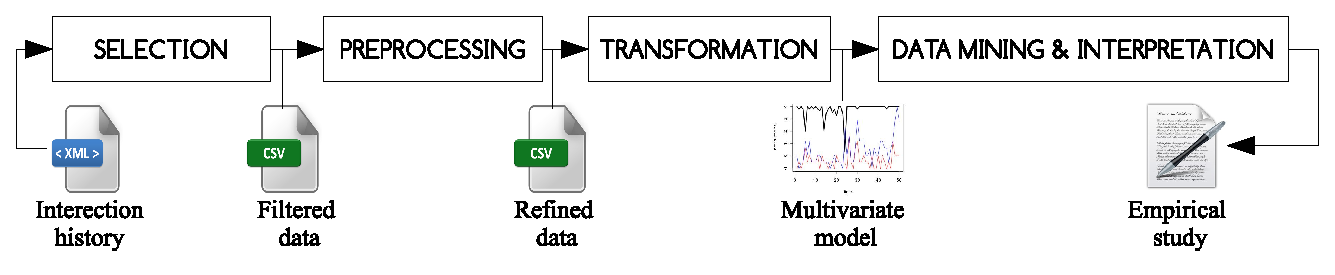
\includegraphics[width=0.9\linewidth,clip=,angle=0]{figures/phases} 
%\end{tabular}
%\caption{Schematization of phases involved in our study.}
%\label{fig:esq}
%\end{figure*}


\section{Mylyn Data Description}

\subsection{Mylyn Data}
For our analysis, we used the Mylyn dataset of development data.  Mylyn \cite{KM06} is an Eclipe plugin that monitors the program elements a programmer interacts with in order to build a task context. A subset of Eclipse developers (principally from the Mylyn and PDE Eclipse projects) use the Mylyn Monitor tool to capture fine-grained usage data of their IDE that they attach to the bug fixes as a task context they submit to Eclipse. This allows reviewers of the bug fixes to use the same task context when they review the changes. The task context contains the entire interaction history since a developer activated the task he or she was working on, and as such is a rather reliable account of IDE usage over time (barring a few issues explained below).


To collect the data, we crawled the bugzilla data of the Eclipse project (\url{http://bugs.eclipse.org}), and downloaded all the bugs that had as an attachment a Mylyn task context.  In total, there were 6,182 bug reports which contained 8,102 Mylyn task contexts.


%\subsection{Bugzilla bug reports}
%Bugzilla is a Web-based tool for bug tracking and is installed as a plugin in Eclipse (\textit{http://bugzilla.org}).  This tool is used to organize and manager the solution of software defects and delegate responsibility to programmers. Bugzilla generates files XML call-bug reports, which maintain relevant information about the bugs that occurred.  The traces of interaction history are associated to each bug  report as an attachment.

\subsection{Interaction History Format}
The interaction history is a sequence of ordered events in time~\cite{YR11}.  An event is associated to a direct action of the programmer in program elements, for instance: edit and selection events. Other interaction events are indirect \cite{KM06}: they are issued by Mylyn itself while it is maintaining its DOI model of a programmer's task context. However these events are not edit or selection events. Each event captures several pieces of information: the timestamp, the kind of event and the signature of the code element that was interacted with (package, class, attribute, or method signature---including name and parameters). 

In Table \ref{tbl:kind_event} we show the different kinds of events and their description; in Table \ref{tbl:sample_event} we show an example of an interaction history. However, certain characteristics in the data present challenges around the data mining we plan to perform \cite{MFR14}. These cases must be detected and resolved in order to get a representative time series model of programmer activity. We describe these issues and our solutions below.


\begin{table}[ht!]
\small
\renewcommand{\arraystretch}{1.3}
\caption{Kinds of interaction events~\cite{KM06} in Mylyn. }
\label{tbl:kind_event}
\centering
\begin{tabular}{|p{1.7cm}|p{1.3cm}|p{8cm}|} 
  \hline 
kind & mode & description \\  
  \hline 
    \hline 
selection & direct &  Editor and view selections via mouse \\
edit & direct & Textual and graphical edits  \\
command & direct & Operations such as saving, building, preference setting  \\
manipulation & direct & Direct manipulation of interest  \\
propagation & indirect & Interaction propagates to structurally related elements  \\
prediction & indirect & Capture of potential future interaction events \\
  \hline
\end{tabular}

\end{table}


\begin{table}[ht!]
\small
\renewcommand{\arraystretch}{1.3}
\caption{ Example of interaction history. }
\label{tbl:sample_event}
\centering
\begin{tabular}{|c|l|c|c|c|} 
  \hline 
    & StartTime & EndTime & EventKind &  Method  \\
  \hline
  \hline
  1 & 10:30:00 & - & selection & m1  \\
  2 & 10:30:40 & - & manipulation & - \\
  3 & 10:30:40 & - & edit & m1  \\
  4 & 10:31:03.700 & - & selection & m1  \\
  5 & 10:31:03.800 & - & selection & m2  \\	  
  6 & 10:31:03.850 & - & selection & m3  \\	  
  7 & 10:32:05 & 10:33:07 & edit (5) & m2  \\	  
  8 & 10:33:10 & - & prediction & - \\
  \hline  
\end{tabular}
\end{table}



\subsection{Special Characteristics of Mylyn Data}
 Below, we describe the characteristics of Mylyn data one has to consider before processing them. This is especially relevant in our case since our study needs a representation of the activity as close to reality as possible.  In Section \ref{sec:trans} we describe the criteria used to process these characteristics. 


\textbf{Aggregate events. } This type of event includes several actions on the same program element. These actions usually occur within an interval of short duration time.  Whenever an aggregation occurs, the event is expanded to include two timestamps defining a range of time, instead of a single timestamp, and a number of events. Accordingly, these aggregate events lose their specific time besides the range of time. The reason of this is that for scalability---in terms of storage---Mylyn does not register all the user events.

For example, Table \ref{tbl:sample_event} shows an aggregate edit event in row 7. We indicate in parenthesis the number of actions associated and the field \textit{EndTime} registers the timestamp of the last occurrence. Clearly, too much aggregation in a given trace severely compromises the detection of work fragmentation as this relies on accurate timestamps.


\textbf{Massive events. } Such an event occurs when the same action is executed on more than one program element in a very short time. This massive action generates consecutive events of the same kind and with a tiny gap between them.

For example, massive events are produced when we select an entire group of classes from the navigation tree panel in Eclipse. In  Table \ref{tbl:sample_event} we show a massive selection on the methods m1, m2 and m3  in rows 4, 5 and 6. This massive selection produces three consecutive events with a time gap of not more than 0.1 seconds. These events overstate the activity of developers as each of these does not correspond to an individual developer action; rather, the entire sequence is.

\RR{Perhaps another example here: it was not clear for one of the reviewer why this was necessary. E.g.: if I scroll down in the outline view with the keyboard I will be generating many selection events. Check other characteristics too (agregate, long).}

\textbf{Very long events. } These events have a duration time ($|EndTime - StartTime|$) much larger than the mean. This mainly occurs in aggregate events. We believe that this issue is due to factors related to Mylyn, since it can register the end time of an event when the task is resumed after a long downtime. Another cause of these events is when one selects a code fragment and maintains this action for a long time. 
 
After exploring a sample of traces, we noticed that a long interruption of activity implicitly splits a trace into two sub-traces.  Moreover,  we have realized that many long events happen around this border. That is, they began before the interruption and finished immediately after the interruption, which confirms the observation above (resumption of a task after a long downtime). However this has the side effect of hiding the gaps of activity in the sequence of events if care is not taken. Consequently, the duration of these events is overstated; however, finding their actual duration is not trivial. 
%was extended beyond the significant real time, since it implicitly encapsulated  an interruption in its execution interval. 

\subsection{Selection}
We used the phases of the process \textit{Knowledge Discovery in Databases (KDD~\cite{FPP96})} to discover useful knowledge from our collection of data: we first select data, then preprocess it, before transforming it to time series.

Our purpose is the analysis of work fragmentation and interruptions in software development. Therefore, we focused only in the interaction data of the user with the program elements. The  variables of interest for our study are~\cite{RD13}:
\begin{enumerate}
	\item Duration: the time that a programmer took to perform a programming task. 
	\item Edition:  the amount of code changes that were necessary to perform said task. %It is associated to the  edit events.
	\item Navigation: how many program elements were consulted in a task; represented by selection events.
	\item Edit ratio: as in previous studies \cite{KM06}, the ratio of edits over edits and selections is an indicator of more efficient work since program exploration is reduced.
\end{enumerate}

First, we have kept only the edit and selection events that are associated to a program element. These type of events are distributed in 8058 traces. On the other hand, edit-type events also occur when the programmer double clicks on a file. In these events the starting time and ending time are the same~\cite{LJD11}. We consider that the double-clicking actions form part of the user navigation, therefore these events are transformed into selection events.  

Second, we have kept all traces without aggregate information. Unfortunately, we cannot know the distribution in time of the actions that have been aggregated in a single event: without additional information, an aggregation of 15 events over one hour is as likely every 4 minutes as it is to have 10 events in the first 5 minutes and 5 more in the last 10 minutes. Therefore, designing a correct disaggregation task to this traces is very difficult, if not impossible.

In order to keep as many traces as possible, we have also kept a little group of traces with aggregate information where the aggregate events have a maximum duration time of five minutes (to minimize uncertainty) or have only two aggregate actions (since the actual event timestamps are known in this case). Thus, we were left with 6260 traces.

It could be possible that these traces we discarded were biased in one way or another. In Figure~\ref{fig:hist_rejected}, we note that in our data the traces with aggregation information appear from  the year 2008 on, and slowly increase in frequency from then. We would expect such a pattern from a change to the version of Mylyn, rather than a change to the type of tasks being performed. This is corroborated with our tests of a recent version of Mylyn, which seems to be even more aggressive in discarding information (it only keeps information at the class level, discarding method level information). As such, our assumption is that it is unlikely that this change is due to anything else than the version of Mylyn that was in use (and hence is not due to different tasks, people, etc). This leads us to believe that it is unlikely that filtering these traces would introduce other sources of bias.

%We assume the programmers used newer versions of Mylyn, which included the aggregation for grouping of collapsed events. Furthermore, 


\begin{figure}[!ht]
	\centering
	\begin{tabular}{c}
		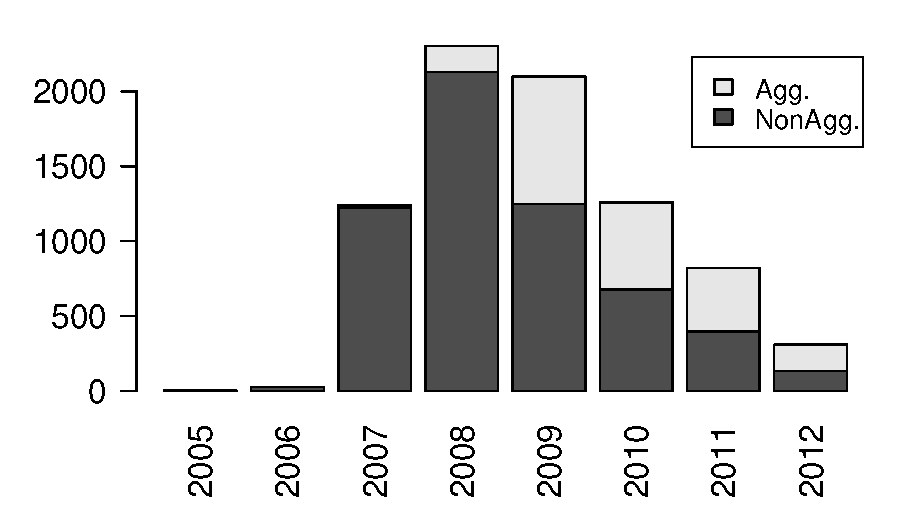
\includegraphics[width=0.5\linewidth,clip=, angle=0]{figures/hist_rejected} 
	\end{tabular}
	\caption{Grouping by date all the traces, with aggregate information (light gray) and without aggregate information (dark gray).}
	\label{fig:hist_rejected}
\end{figure}

Finally, we found that 26\% of traces had at least an interruption over 8 hours, which is hence large enough to represent the difference between two working days. In these cases, we treated these long activity gaps as splitting points in order to decompose a long trace in several development sessions \cite{RL07}. 

After this, we considered a minimum duration time of 30 minutes in order to ensure a minimum of activity during a session. In this way, we obtained a final total of 4284 useful sessions to be processed in the next phase. 


\subsection{Preprocessing}\label{sec:trans}
After filtering out traces, we describe the final processing steps that yield the final development \emph{sessions} that we study:

\textbf{Sorting.} We sort chronologically all the events by their starting time. Before that, we normalize the timezone of each trace. We found 156 traces (3\%) with more than one timezone.  

\textbf{Massive events.} We use a short spacing interval to join consecutive massive events in only two, the first and the last event (Figure \ref{fig:mass_event}). We have considered a spacing size of 0.1 seconds (100 milliseconds). All the massive events we found were of type ``selection", which concurs which our observation above (multiple selection of several entities at the same time). The total number of selection events was reduced by 45\%.
% es una caracteristica mas comun de las selecciones, por lo tanto queremos minimizar el caso de edits. Con 0.1 logramos 

\begin{figure}[t]
	\centering
	\begin{tabular}{c}
		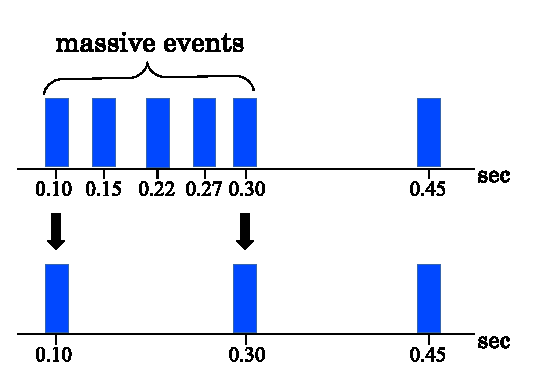
\includegraphics[width=0.5\linewidth,clip=, angle=0]{figures/mass_event} 
	\end{tabular}
	\caption{Replacing five massive events with only two events.}
	\label{fig:mass_event}
\end{figure}

\textbf{Disaggregation.} We disaggregate all the actions associated with each remaining aggregate event with equidistant separation, as was done by Ying and Robillard \cite{YR11}. Due to the filtering above, this was only applied on traces that had aggregate events of short duration ($\leq$ 5 minutes).

\textbf{Event splitting.} Finally, we split all the long duration events to better fit a time series model, which is composed of a series of actions in specific times with intervals of the same duration. A normal event does not generally have duration (EndTime is null). However, 12\% of normal events  had a duration $> 0$ seconds and 3\% $\geq$ 1 hour, these events are outliers. Therefore, we split each long event in two events: one at the start and the other at the end of the interval. This is the same criteria applied for massive and aggregate events.

Table \ref{tbl:mass_events} shows the ratio of variation of the number of events after preprocessing.

\begin{table}[hb!]
	\small
	\renewcommand{\arraystretch}{1.3}
	\caption{Number of events after preprocessing.}
	\label{tbl:mass_events}
	\centering
	\begin{tabular}{l | c | c | c } 
		type event & before & after & \% variation  \\  
		\hline 
		edit &	 452,236 & 475,554 &	+5\%   \\
		selection &	658,768 & 527,652 & -20\%   \\
		\hline
		total & 1,111,004 & 1,003,206 & -10\%  \\
	\end{tabular}
\end{table}

\subsection{Transformation}
Our goal is to build compact and representative models from each session. In this sense, we used aggregation of events to generate a multivariate time series (MTS). An MTS is a sequence of multivariate observations taken at continuous time intervals coming from a same phenomenon. We build the MTS with edit and navigation variables; the time unit is the minute, and every observation is the sum of all the events that occurred in this minute. We selected the minute as unit time because it seemed to be an appropriate and minimal representation of the user interaction in a programming task---obviously a subjective decision. 

Creating time series is a useful way of representing temporal data because they allow us to apply clustering techniques and find recurrent patterns; in our case every minute of the time series contains different observation, which is the reason why we created multivariate time series. This way we can model a session as a MTS, where every minute contains the quantification of edition and selection events. The partition of the data into sessions do not alter the results since we are interested in the values by minute, so having longer sessions do not necessarily increase the number of events per minute.

%\RR{motivate more the time series stuff}

Mylyn data has another characteristic which is unusual for time series: the time of occurrence of the events is not periodic (see column \textit{StartTime} in Table \ref{tbl:sample_event}). That is to say, events occur with non-equidistant separation gaps between them. However, in a time series, the values must be evenly spaced and chronologically sorted. For this reason, we compressed the size of the multivariate time series, pulling apart all the interruptions as a new time series variable. Then, each time series value represents the interruption duration in this minute (Figure \ref{fig:trans}). 


Consequently, the temporal component represents the \textit{real working time} of a programming task, excluding inactivity. This allows us to compute our activity indicators (number of edits, selections, edit ratio) independently of the amount of inactivity in a session.
% That is to say, each consecutive unit time corresponds to a minute of user activity, where there was at least one event of edit or selection. 
\paragraph{Defining an interruption.}An important task during the transformation phase is to identify the interruptions along a working session. In this study we use two kind of interruptions, and we define them as follows:

\begin{itemize}
	\item \textit{Interruption. }We define empirically an interruption as a pause of programming of duration $\geq 3$ minutes. This is based on previous work where we observed that short interruptions lasted usually this long \cite{GM04}. 
	
	\item \textit{Prolonged interruption. }Based on additional observations from this work, we defined a prolonged interruption as one lasting for more than 12 minutes. These thresholds are also supported by the Activity Theory models of Kaptelinin and Nardi \cite{KaptelininN07}. This study presented work fragmentation at two different levels: actions and activities. Interruptions originated after a period of around three minutes of sustained attention to the previous action were considered when people were switching at the level of interactions with artifacts of people. Interruptions originated after a period of twelve minutes of sustained attention to a previous activity where considered when people were switching at the level of interactions with projects or topics.  
\end{itemize}


%\RR{Add emphasis to the paragraph above since reviewers missed it (asking for motivation for the thresholds)}

We identified that 98\% of sessions had at least one gap of activity. Moreover, we observe that the short interruptions predominate over the prolonged interruptions (Table \ref{tbl:by_duration}). This first result tells us that work fragmentation is extremely prevalent in our dataset.

\begin{table}[ht!]
	\small
	\renewcommand{\arraystretch}{1.3}
	\caption{Prevalence of interruptions according to their duration time. }
	\label{tbl:by_duration}
	\centering
	\begin{tabular}{p{3cm}|p{0.8cm}|p{6cm}} 
		duration & ratio & examples  \\
		\hline   
		$[3  - 12 min \rangle$ & 69\% & short pause, answer a question, thinking, looking for interruption  \\ 
		\hline 
		$[12  - 30 min \rangle$ & 18\% & coffee break, short meeting, extended interruption  \\
		$[30 min - 2 hr \rangle$  & 9\% & lunch break, a meeting  \\
		$[2 hr - 8 hr \rangle$ & 4\% & extended meeting \\
		%$[8 hr - \infty \rangle$ & 0.14 & \textit{a long interruption}   \\
		%$[8 hr -  \infty \rangle$ & 0.06  &  a weekend \\
		%$[2 day - \infty \rangle$ & 0.04 & a long holiday \\ 
	\end{tabular}
\end{table}

\begin{figure}[t]
	\centering
	\begin{tabular}{c}
		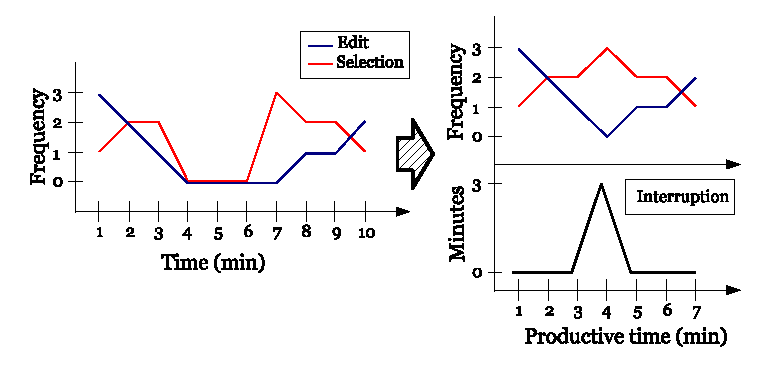
\includegraphics[width=.6\linewidth,clip=, angle=0]{figures/trans} 
	\end{tabular}
	\caption{Example of how to compress a time series. }
	\label{fig:trans}
\end{figure}


After the transformation phase, we had the sessions in a proper format to carry out the analysis. In the Figure \ref{fig:mylyn_sessions_stats} we can observe some statistics (left) about the sessions in Mylyn and the distribution (right) of the productive time. The productive time of the session is the total time without considering the time consumed by interruptions. Also, the outliers are ignored by setting a threshold of three times the standard deviation. This filter is used only to show the distribution and avoid a very long tail provoked by unusually long sessions.


\begin{figure}
	\centering	
	\begin{minipage}[c]{0.30\linewidth}
		\small
		\centering
			\begin{tabular}{| p{2cm} |p{2cm} |} 
				\hline 
				stat & value \\  
				\hline 
				\hline 
				total & 4,284 \\
				min. & 2 min \\
				1st Qu. & 18 min\\
				median & 35 min \\
				mean & 48.91 min \\
				3rd Qu. & 62 min \\
				max. & 535 min\\
				\hline
				
			\end{tabular}
	\end{minipage}
	\begin{minipage}[c]{0.60\linewidth}
		\centering
		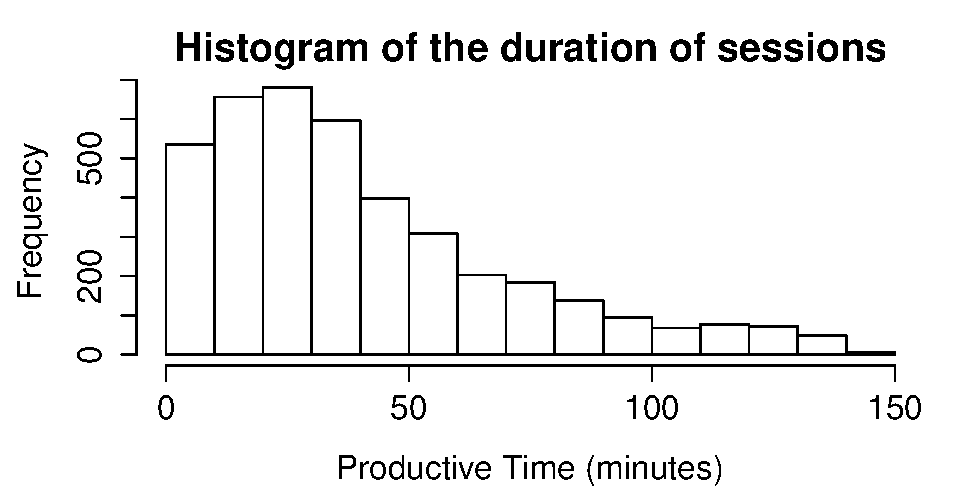
\includegraphics[width=0.8\linewidth,clip=, angle=0]{figures/mylyn_trace_duration} 
	\end{minipage}
	\caption{Statistics (left) and distribution of the productive time (right) of the sessions in Mylyn}
	\label{fig:mylyn_sessions_stats}
\end{figure}

%\begin{table}[ht!]
%	\small
%	\renewcommand{\arraystretch}{1.3}
%	\caption{Statistics about the sessions in Mylyn. }
%	\label{tbl:stats_sessions_mylyn}
%	\centering
%	\begin{tabular}{| p{3cm} |p{3cm} |} 
%		\hline 
%		stat & value \\  
%		\hline 
%		\hline 
%		total & 4,284 \\
%		min. & 2 min \\
%		1st Qu. & 18 min\\
%		median & 35 min \\
%		mean & 48.91 min \\
%		3rd Qu. & 62 min \\
%		max. & 535 min\\
%		\hline
%		
%	\end{tabular}
%\end{table}
%
%
%\begin{figure}[t]
%	\centering
%	\begin{tabular}{c}
%		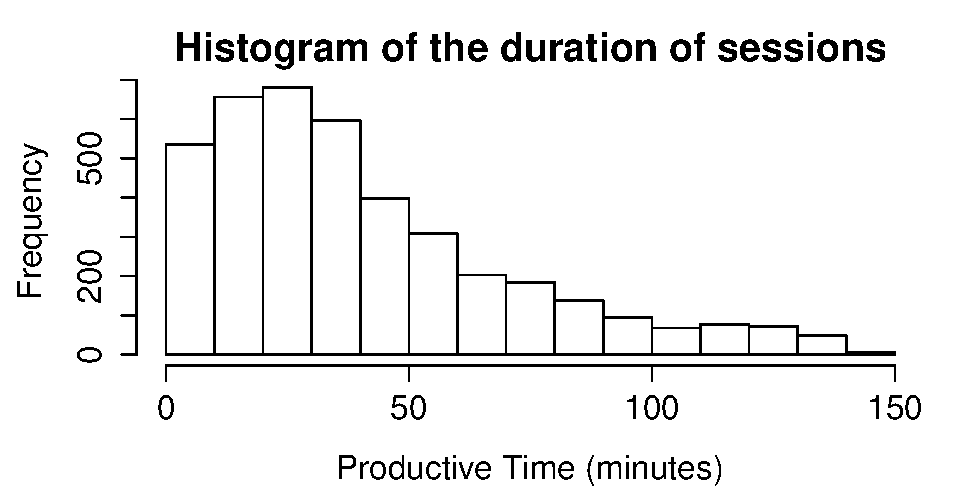
\includegraphics[width=0.6\linewidth,clip=, angle=0]{figures/mylyn_trace_duration} 
%	\end{tabular}
%	\caption{Histogram of the duration of the sessions in Mylyn.}
%	\label{fig:mylyn_trace_duration}
%\end{figure}





\section{Eclipse Usage Data Collector Data Description}

\subsection{The Eclipse UDC}
The Usage Data Collector (UDC) dataset is a large compendium of information about interaction data from users of Eclipse, collected from December 2008 to August 2010, with the intention to keep track of how programmers are using the IDE. The framework listens to the events triggered by the user or the system, such as: edition and navigation commands; the startup of a plug in; or the closing of the platform. To be more specific, UDC collects information about loaded bundles, commands accessed via keyboard shortcuts, actions invoked via menu or tool-bars, perspective changes, view usage and editor usage. The UDC is a large dataset that contains information of around 1,800,000 users, and has a total of 2,323,233,101 unique rows with 5 attributes each. Table \ref{tbl:att_udc} shows a description of the attributes.


\begin{table}[ht!]
	\small
	\renewcommand{\arraystretch}{1.3}
	\caption{Attributes in UDC data. }
	\label{tbl:att_udc}
	\centering
	\begin{tabular}{|p{2.5cm}|p{10cm}|} 
		\hline 
		attribute & description \\  
		\hline 
		\hline 
		userId &  Unique number that identifies a user \\
		what & The action of the event (deactivated, activated, opened, executed, etc.)  \\
		kind & What kind of event was executed (workbench, view, command, etc.)  \\
		bundleId & Description of the event's package  \\
		bundleVersion & Version of the bundle's event  \\
		description & Description of the event\\
		datetime & Date and time in UNIX format\\
		\hline
	\end{tabular}
	
\end{table}

\subsection{Selection}
We used the pre-processed version of the data that is published on Google BigQuery, by Murphy-Hill et al. \cite{SnipesETALASD}. This is an alternative version of the original UDC dataset, which is cleaned and preprocessed, so that the transformation phase is simple and focused on our needs. Due to the magnitude of the dataset we only worked on a fragment of it. We took a random sample of 1,000 users that is larger than the dataset we were able to obtain for the Mylyn study.

The first step was to query the dataset to get the data from 1,000 random users. We delimited the query to obtain only those events dispatched by the user, ignoring system events. We also ignored the bundle version and transformed the UNIX date into a more legible datetime format. From this query we extracted 4,321,349 unique events, which are around $0.18\%$ of the whole dataset.

\subsection{Preprocessing}
After obtaining the data, the next step was to add the attributes required by every event in order to match as closely as possible the format of the Mylyn data; this allowed us to reuse a part of our analysis. Hence, we added fields corresponding to the type of the event (edition or selection), its duration (time elapsing between one event and the next one, used to determine where interruptions take place and sessions end) and an ID to identify the different working sessions present on the data. For the latter, we sorted the data by \textit{userId} and \textit{datetime}. This was required because, by default, the user's data is mixed and we need it not only chronologically correct but also sorted by users to tag the working sessions of every user without interferences. 

It was also required to fill the description for the events that indicate the activation or deactivation of the workbench of Eclipse, but as they were the only events with this error this task was trivial. Additionally, it was needed to classify the events, which was a complicated task.

%With Mylyn we have information about the end time of an event. The UDC dataset doesn't have an attribute to show this information, so we added an interval time in seconds that depends on the next event executed. This is important to identify those events that represent an interruption or the end of a session. 

\subsection{Classification of events}
Mylyn events belong to two main categories: edition and selection. The UDC data doesn't have this, so we inferred a classification manually. Note that we reuse the same term of selection in the following text, as it was used in Mylyn data. Strictly speaking, the word "navigation" would be better suited to the variety of events present in the UDC data, but we keep the old term for consistency.
%To select the event type, we made a thorough analysis of the different events to classify them where they better fit. In comparison with Mylyn we didn't have a classification by default but the attributes can give us a very good approximation.

We took into consideration the attributes \textit{what}, \textit{kind} and \textit{description} to choose the best classification for every event. Starting by the kind attribute, some events are labeled as \textit{view} which are precisely those that open, activate or close a view such as the console, the package explorer or the variables view. Therefore, the events of the kind \textit{view} were classified as selection-type events.

The classification for the rest of the events is more complex: we needed to check directly the command description and the bundle it belongs to in order to precisely infer its meaning (e.g., We could label as edition all those commands with the attributes \textit{command} and \textit{executed}). The majority of them are in fact of that type edition, but some executed commands also can open a view, navigate through the text or go to another class. For this reason we took a closer look into the bundle name and what the description can tell us about the events.

Thus, by default, all events of the attributes \textit{command} and \textit{executed} were classified as edition and afterwards we did a thorough analysis to identify those that are actually selection events. This way we categorized as selection all the events where we could tell (based on the description) if they have the purpose to, for instance, navigate to another window, open a perspective, find and replace words, search code, debugging, or perform window management. The description contains the whole path from the top package to the class that implements the event, so we look for key words to apply the classification. The proportion of events after the classification is shown in the Table \ref{tbl:prop_events_udc}.
We used an iterative process involving two of the authors of the paper to arrive to this result; the process was iterative, until we reached consensus. A sample of the classification can be seen in the Table \ref{tbl:ej_events_udc}.

\begin{table}[ht!]
	\small
	\renewcommand{\arraystretch}{1.3}
	\caption{Proportion of events. }
	\label{tbl:prop_events_udc}
	\centering
	\begin{tabular}{|p{1.7cm}|p{2 cm}|} 
		\hline 
		event & percentage \\  
		\hline 
		\hline 
		edition &  $34.6\%$  \\
		selection & $31.1\%$ \\
		system & $31.5\%$  \\
		control & $0.8\%$  \\
		\hline
	\end{tabular}
\end{table}

\begin{table}[ht!]
	\small
	\renewcommand{\arraystretch}{1.3}
	\caption{Sample of classified events in UDC. }
	\label{tbl:ej_events_udc}
	\centering
	\begin{tabular}{|p{6cm}| p{2 cm} |} 
		\hline 
		description & type \\  
		\hline 
		\hline 
		org.eclipse.ui.edit.delete & edition \\
		org.eclipse.ui.file.save & edition \\
		org.eclipse.ui.edit.undo & edition \\
		org.eclipse.jdt.ui.CompilationUnitEditor & selection \\
		org.eclipse.ui.console.ConsoleView & selection \\
		org.eclipse.debug.ui.commands.StepOver & selection \\ 
		org.eclipse.ui.workbench & system \\
		org.eclipse.team.sync.views.SynchronizeView & control \\
		\hline
	\end{tabular}
\end{table}

The edition and selection types are the ones we are interested for this study. The system classification is composed of the events that activate and deactivate the workspace of Eclipse; it is difficult to determine when and why these events are executed (they can be executed either via user or system action, and the order of execution in relation with associated events is not clear), so we decided to establish this particular classification for them. Finally, the events of the type control are those related to the version control system. 

\subsection{Transformation}
Once the events were classified and sorted, we split the dataset into sessions, defining a session as a period of registered work between interruptions of 8 hours or larger, as we did with Mylyn. We split the data by users to avoid a conflict between the last event of a user and the first one of another. After this, we obtained a total of 28,989 different sessions; but after a filter to keep only those with at least 30 minutes of productive time (as we did with the Mylyn dataset), we ended up with 15,825 useful sessions, in contrast with the 4,284 we had from Mylyn. On average, every session contains 154 edition and selection events, and this number is positively correlated (0.81) with the size of the session. This is an expected result, as having more time consequently increases the number of events in the session. Additionally, it is important to remark that the number of events in a session do not alter the edit or selection events per minute.

To identify an the interruptions on every session, we considered the same definition we used with Mylyn, where an interruption is a segment of 3 minutes or more with no activity registered. 

At this point, we had the same format of sessions with both datasets. In the Figure \ref{fig:udc_sessions_stats} we can see statistics about the sessions (left) and a histogram (right) of the duration of the sessions in UDC, which ignores outliers by setting a threshold of three times the standard deviation.

\begin{figure}
	\centering	
	\begin{minipage}[c]{0.30\linewidth}
		\small
		\centering
		\begin{tabular}{| p{2cm} |p{2cm} |} 
			\hline 
			stat & value \\  
			\hline 
			\hline 
			total & 15,825 \\
			min. & 2 min \\
			1st Qu. & 11 min\\
			median & 23 min \\
			mean & 35.87 min \\
			3rd Qu. & 47 min \\
			max. & 1,345 min\\
			\hline
			
		\end{tabular}
	\end{minipage}
	\begin{minipage}[c]{0.60\linewidth}
		\centering
		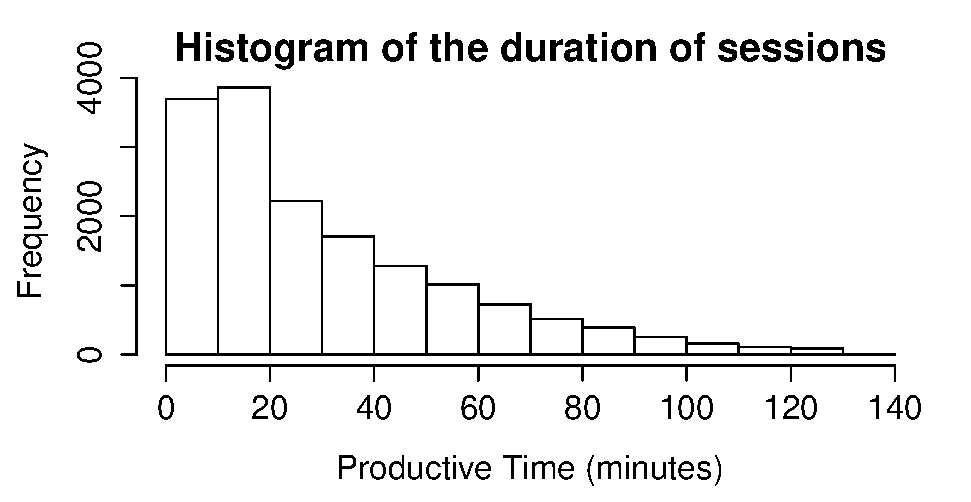
\includegraphics[width=0.8\linewidth,clip=, angle=0]{figures/udc_trace_duration} 
	\end{minipage}
	\caption{Statistics (left) and distribution of the productive time (right) of the sessions in UDC}
	\label{fig:udc_sessions_stats}
\end{figure}


\subsection{Metrics Used in This Study}
Before introducing the results about the first research question, it is convenient to present the metrics used in this study.
We use the following six metrics to measure interruptions and productivity, while controlling for the unproductive time in a session, the length of time of the session itself, and the efficiency of the development that took place during the session.
\\

Metrics characterizing interruptions:
\begin{itemize}
	\item \textit{Number of interruptions}:  counts all the interruptions that occur in a development session.
	\item \textit{Duration of interruption}:  it is the time duration in minutes of the each interruption. 
\end{itemize}

Metrics characterizing productivity and activity:
\begin{itemize}
	\item \textit{Productive work time:} the duration of a development session, subtracting the duration of all the interruptions present in the session, to control for inactivity.
	\item \textit{Number of edits per minute:} the total number of edits events, divided by the productive work time to control for length of the session. This is an indicator of user activity during the session.
	\item \textit{Number of selections per minute:} is the total number of selection events, divided by the productive work time. Also an indicator of activity.
	\item \textit{Edit ratio:} the number of edits divided by the sum of edits and selections, as used by Kersten and Murphy \cite{KM06}; an efficient developer spends less time exploring code and more time editing it.
\end{itemize} 

We measure the effects on productivity using mainly the edit and selection events per minute as indicators. The edit ratio might be also a good indicator, under the assumption that a productive programmer will execute more editing activities than selection or navigation events. However, this is not always the case, given that depending on the role of the worker, selection events can be equivalent to the usage of a designing or reporting tool.

An important reason to consider the edit ratio is that having an interruption requires doing activities that might increase the execution of selection events, reducing the edit events. For example reading the code, navigating around files and starting a debugging sessions are activities heavily loaded of selections events and are common activities after an interruption, according to observational studies. The edit ratio can tell us when there is a reduction of edit events due to (mainly) selection events.

We did a correlation analysis involving the three metrics used (Table \ref{tbl:corr_analysis}, classifying the data between traces with or without interruptions. We find that the Edit/min and Sel/min metrics have low correlation coefficients, which is the expected result. The same happens between the Sel/min and Edit ratio metrics with the data of both kind of traces. The Edit/min and Edit ratio correlation coefficient is higher in both groups, but not high enough to not consider the latter, for it tells something different from the user activity.

\begin{table}
\small
\renewcommand{\arraystretch}{1.3}
\caption{Correlation analysis of the metrics used in the study.}
\label{tbl:corr_analysis}
\centering
\begin{tabular}{|p{4cm}|p{2cm}|}
	  \hline 
	metrics & correlation \\  
	  \hline 
	\multicolumn{2}{c}{\textit{Traces without interruptions}} \\
	    \hline 
		Edit/min vs Sel/min &  0.25  \\
		Edit/min vs Edit ratio &  0.65\\
		Sel/min vs Edit ratio & -0.38  \\
	    \hline 
	\multicolumn{2}{c}{\textit{Traces with interruptions}} \\
	    \hline 
		Edit/min vs Sel/min &  0.35  \\
		Edit/min vs Edit ratio &  0.60\\
		Sel/min vs Edit ratio & -0.32  \\
	    \hline
\end{tabular}
\end{table}


%\RR{motivate more edit ratio, and add here the correlation analysis}

%\begin{table}[ht!]
%	\small
%	\renewcommand{\arraystretch}{1.3}
%	\caption{Statistics about the sessions in UDC. }
%	\label{tbl:stats_sessions_udc}
%	\centering
%	\begin{tabular}{| p{3cm} |p{3cm} |} 
%		\hline 
%		stat & value \\  
%		\hline 
%		\hline 
%		total & 15,825 \\
%		min. & 2 min \\
%		1st Qu. & 11 min\\
%		median & 23 min \\
%		mean & 35.87 min \\
%		3rd Qu. & 47 min \\
%		max. & 1,345 min\\
%		\hline
%		
%	\end{tabular}
%\end{table}
%
%
%
%\begin{figure}[t]
%	\centering
%	\begin{tabular}{c}
%		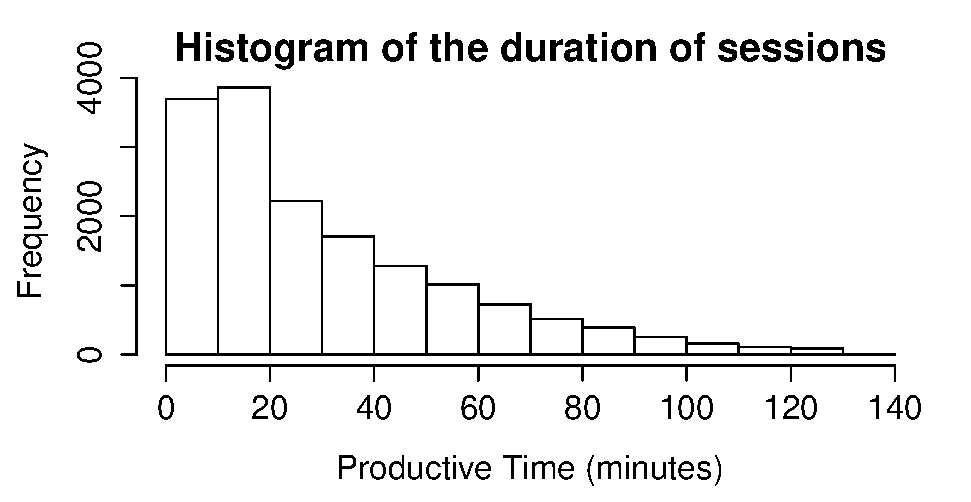
\includegraphics[width=0.6\linewidth,clip=, angle=0]{figures/udc_trace_duration} 
%	\end{tabular}
%	\caption{Histogram of the duration of the sessions in UDC.}
%	\label{fig:hist_session_duration_udc}
%\end{figure}

%After processing the data, we were able to reuse the same data analysis pipeline we used for Mylyn, in order to verify whether the results hold with this other dataset.



%\section{Preview Phases for Knowledge Discovery}
%We used the phases of the process \textit{Knowledge Discovery in Databases (KDD~\cite{FPP96})} to discover useful knowledge from our collection of data: we first select data, then preprocess it, before transforming it to time series. We close this section by presenting the metrics we use in this study. %  (see Figure~\ref{fig:esq}). 
%


%Completed this process, we obtained a set of multivariate time series models to be used in different mining tasks.


%After, we applied smoothing using local means to help us see a clearer signal (discover trends).


%\section{Data Mining and Interpretation}
%In this section, we analyze the effect of the interruptions and work fragmentation in software development by means of exploratory and statistical analysis. To get a better view of the data, we first start by exploring the prevalence of interruptions and their relations with the productive time, before answering our research questions.

\section{RQ1: Relationship between Interruptions and Productivity}



%\subsection{Effect in the productive work time}

%In this section, we explore the relationship between interruptions and the productive time (that is, the time spent in a development session excluding interruptions). Figure \ref{fig:prod_int} is a scatterplot in which the x-axis indicates the number of interruptions and the y-axis indicates the productive work time; both are in logarithmic scale. The brown line emphasizes the lower limit in the relation of both variables: if a trace has $n$ interruptions, then, its minimum productive time is $n+1$ minutes. The graph shows that there is not a very significant relation between the number of interruptions and the productivity time.

%For instance, there are traces with a single interruption and  their productive time up to $2^8$ minutes ($\approx$ 4.3 hours). 

%\begin{figure}[!ht] \centering \begin{tabular}{c}
%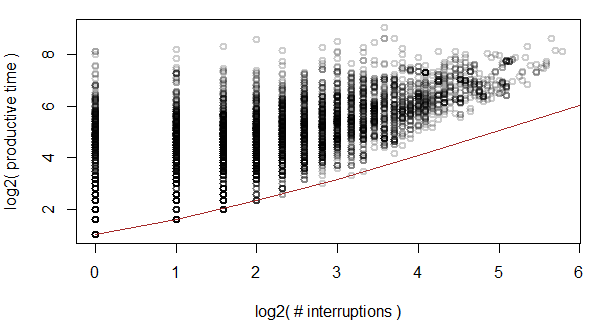
\includegraphics[width=.9\linewidth,clip=, angle=0]{figures/prod_int.png} 
%\end{tabular} \caption{Number of interruptions vs the productive work time. } \label{fig:prod_int} \end{figure} 

%In the second scatter plot, we plot the total duration of the in the x-axis and the productive time on the y-axis (Figure \ref{fig:prod_dura}). We observe a higher average of productive time in traces that had a lesser amount of interruptions. For instance, the traces that have accumulated $\leq 16$ minutes in interruptions, their productive time was $\geq 15$ minutes. Then, according as the duration increases, traces with a lower productive time were appearing. Thus, for example, we found 73 traces that had one interruption $\geq 28$ minutes but only two minutes of productive time. Therefore, we can appreciate a slight effect of long interruption duration over the productive time of the traces. 

%\begin{figure}[!ht] \centering \begin{tabular}{c}
%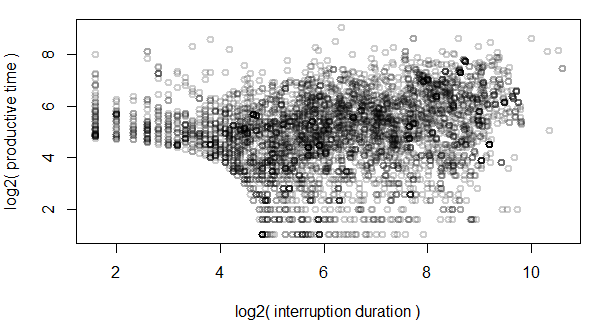
\includegraphics[width=.9\linewidth,clip=, angle=0]{figures/prod_dura.png} 
%\end{tabular} \caption{Total duration of interruptions vs the productive work time.. } \label{fig:prod_dura} \end{figure}



\subsection{Relation between Interruptions, and Edits and Selections}

As mentioned above, we use the metrics of edit, selection, and edit ratio as indicators of productivity. We first examine the number of edits and selections, and how their distribution varies in function of the number and type of interruptions.
 %we assume that the productivity is in function of the number of edit and selection events that the programmer performs in a trace. 

%First, we analyzed the number of interruptions over the productivity. In this sense, 
We split the data in five groups: The first group contains all the sessions without interruptions (\textit{none}). For the others groups, we have considered four ranges of number of interruptions delimited by their quartiles; the results differ between Mylyn and UDC, existing more interruptions per session in the former (Table \ref{tbl:quartil_int}). Then, for each group, we display the distribution of events per minute and edit ratio via boxplots. We can see the results with Mylyn in Figure \ref{fig:box_int_events}), and for UDC in Figure \ref{fig:box_int_events_udc}.

In the results with Mylyn, we observe a large difference between the sessions without interruptions and the ones who do. Further, we observe that the rate of events per minute decreases slightly when the session has more interruptions. Therefore, we can intuit that the relationship between number of interruptions and the productivity indicators that are edits and selections, tends to be inversely proportional. 

With UDC, the results show a similar pattern in comparison with the results with Mylyn. When facing zero interruptions the editions and selections per minute are greater than with one or more interruptions, and as more interruptions occur this metrics gradually decrease. The difference between sessions with no interruptions and at least one is less marked in the edit per minute metric, but the selections per minute metric is more alike to the Mylyn results.


\begin{table}[ht!]
\small
\renewcommand{\arraystretch}{1.3}
\caption{Thresholds used to group sessions based on their number of interruptions} %separate the data in four percentages groups regarding the number of interruptions in each trace.}
\label{tbl:quartil_int}
\centering
\begin{tabular}{l | p{0.6cm} | p{0.6cm} | p{0.6cm}} 
     & $25\%$ & $50\%$ & $75\%$ \\  
  \hline 
  Mylyn &  3 & 5 & 10  \\ 
  \hline  
  UDC &  2 & 4 & 7  \\  
\end{tabular}
\end{table}


\begin{figure}[!ht]
\centering
\begin{tabular}{c}
\minipage{0.33\textwidth}
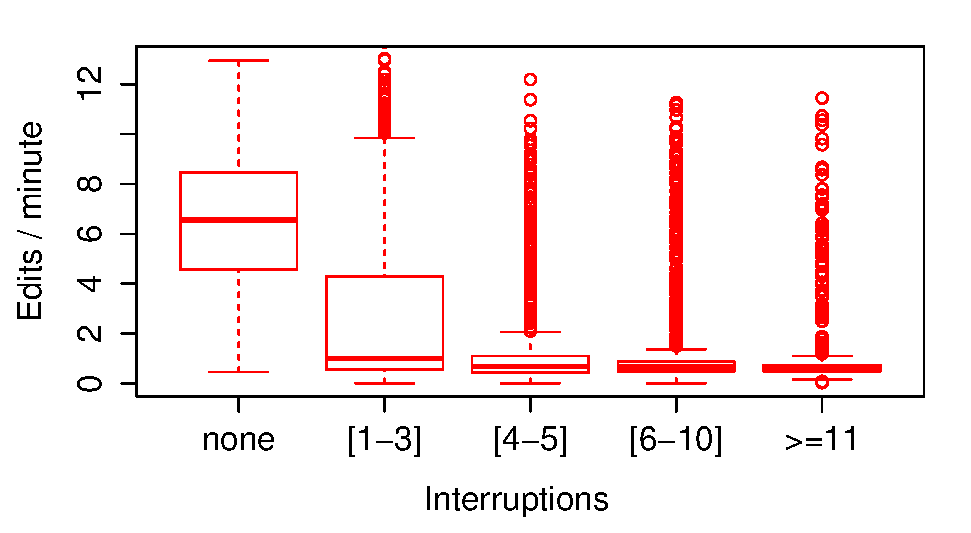
\includegraphics[width=\linewidth,clip=, angle=0]{figures/box_int_events_edit}  
\endminipage\hfill
\minipage{0.33\textwidth}
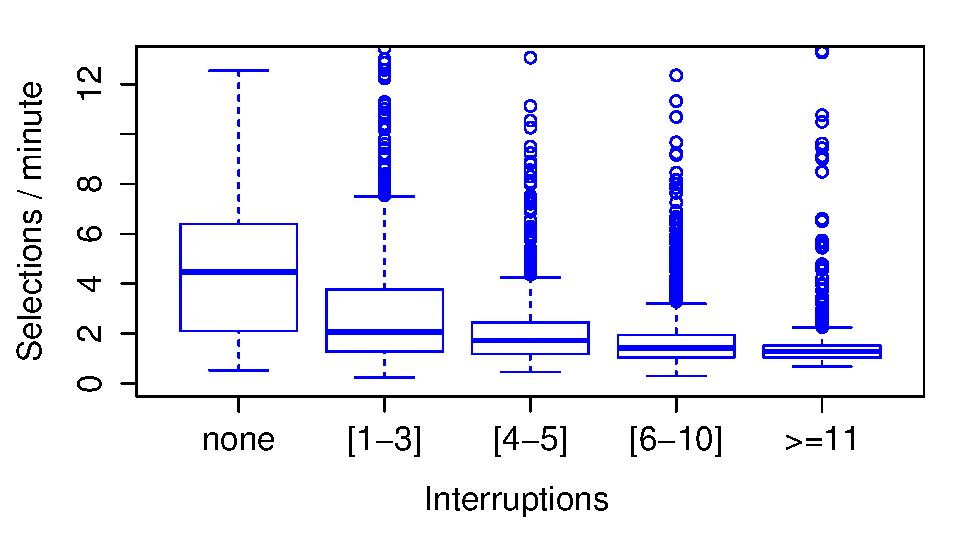
\includegraphics[width=\linewidth,clip=, angle=0]{figures/box_int_events_sel}  
\endminipage\hfill
\minipage{0.33\textwidth}
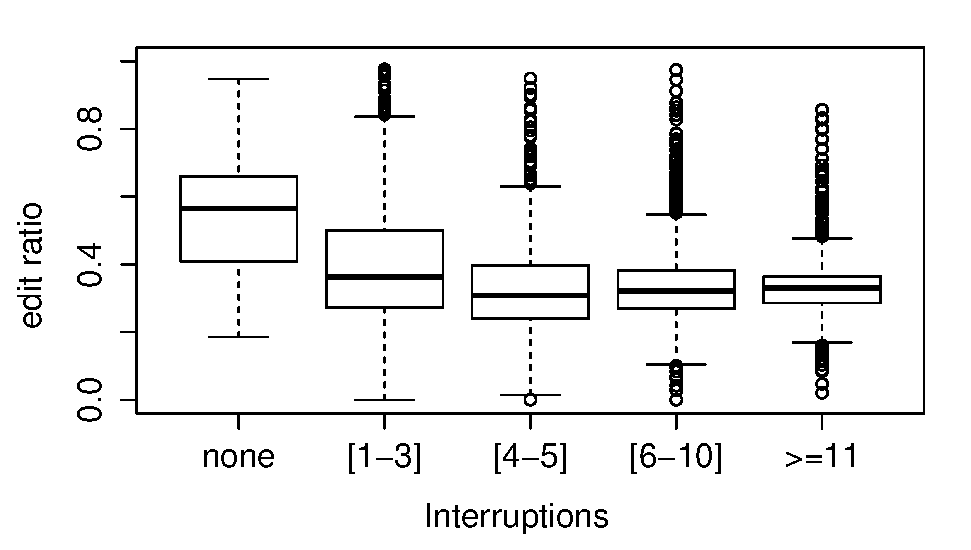
\includegraphics[width=\linewidth,clip=, angle=0]{figures/box_int_ratio} 
\endminipage\hfill
\end{tabular}
\caption{Boxplots showing the relation between the number of edits and selection events per minute, the edit ratio, and the number of interruptions in Mylyn. }
\label{fig:box_int_events}
\end{figure}

\begin{figure}[!ht]
	\centering
	\begin{tabular}{c}
		\minipage{0.33\textwidth}
		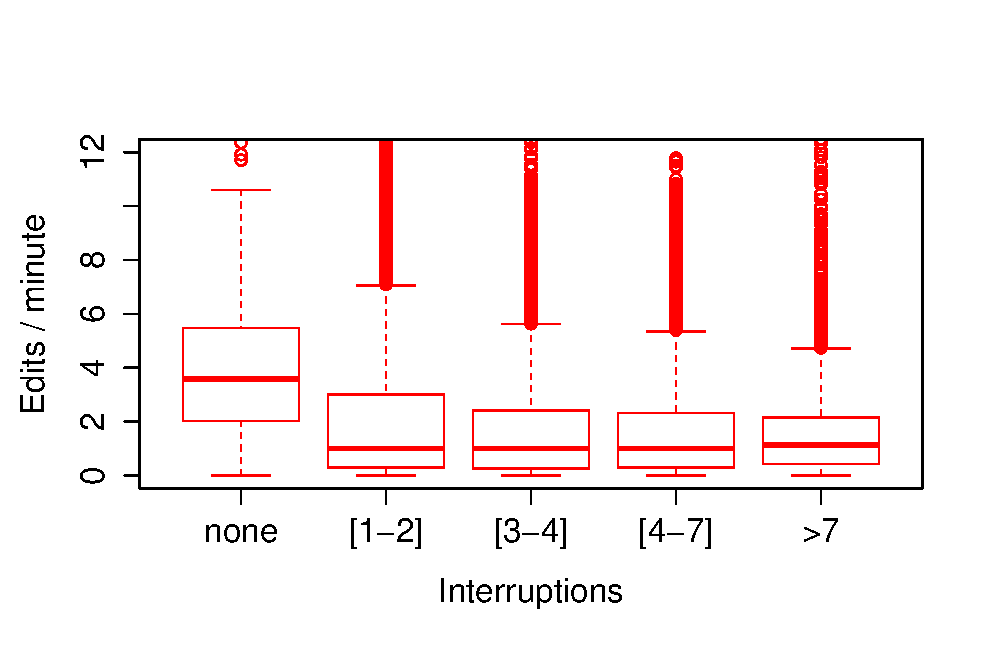
\includegraphics[width=\linewidth,clip=, angle=0]{figures/udc_box_int_events_edit}  \\
		\endminipage\hfill
		\minipage{0.33\textwidth}
		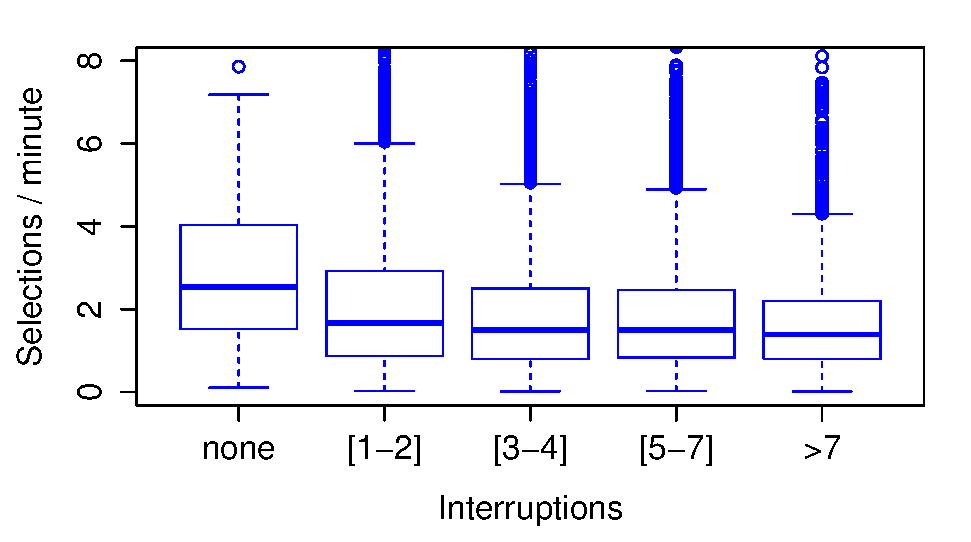
\includegraphics[width=\linewidth,clip=, angle=0]{figures/udc_box_int_events_sel}  \\
		\endminipage\hfil
		\minipage{0.33\textwidth}
		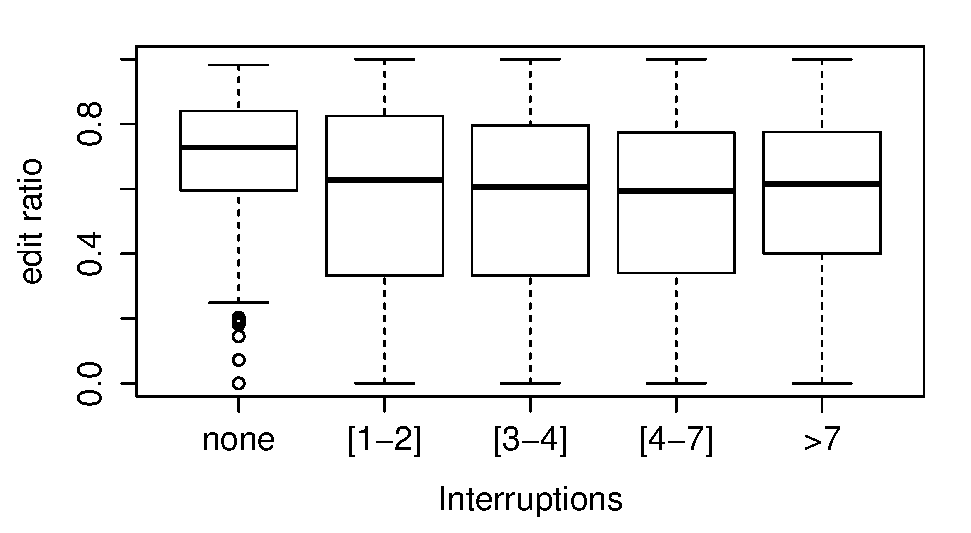
\includegraphics[width=\linewidth,clip=, angle=0]{figures/udc_box_int_events_ratio} \\
		\endminipage\hfill
	\end{tabular}
	\caption{Boxplots showing the relation between the number of editions and selections per minute, the edit ratio, and the number of interruptions in UDC. }
	\label{fig:box_int_events_udc}
\end{figure}

Beyond visual inspection, we also quantify the statistical and the practical significance of these observations. First, in the results with Mylyn, all the differences observed are statistically significant with very low p-values (see Table~\ref{tbl:p_value}) according to the Mann-Whitney U-test. This is not surprising, given the shape of the boxplots and the size of the samples.

More importantly, we used \textit{Cohen's d} to measure the practical significance of these results in term of effect size % the effect size of the differences in means as standardized difference~
\cite{C94}. \textit{Cohen's thresholds} are defined as follows: trivial ($<0.2$), small  ($\langle 0.2 - 0.5 ]$), moderate ($\langle 0.5 - 0.8 ]$) and large effect ($> 0.8$). As shown in Table \ref{tbl:p_value}, we note that the effect size of the interruptions over the number of edits by minute is (very) large. In selections, the effect is moderate for sessions having up three interruptions, and large to very large for sessions with over four interruptions. This reinforces our impressions that interruptions and user activity follow inverse relationships, and that they are quite pronounced.

On the other hand, with the results in UDC, an important difference is that the effect overall appears to be less pronounced in UDC and we can see it on the effect size tests shown in the Table \ref{tbl:p_value_udc}. Most of the observed effects are medium, while in the Mylyn dataset the effects were large. Note that despite the differences in effect sizes, the differences are still significant and it is possible to reach the same conclusions.

%We conclude that the user productivity could be adversely affected by increased interruptions.

\begin{table}[ht!]
\tiny
\renewcommand{\arraystretch}{1.3}
\caption{Effect size and significance of the relationship between number of edit per minute, selection per minute, edit ratio, and number of interruptions on Mylyn data} 
\label{tbl:p_value}
\centering
\begin{tabular}{l | p{0.75cm} | p{1.2cm} | p{1.2cm} | p{1.2cm} |p{1.2cm}} 

   & none & $\leq 3$ & $[4 - 5]$ & $[6 - 10]$ & $\geq 11$  \\  
  \hline
  \multicolumn{6}{c}{\textbf{Edits}} \\
  \hline
  mean & 6.29 &	2.59 & 1.55 & 1.29 & 0.91  \\ 
  % \cline{3-6} 
  %t.test & $\hookrightarrow$& \multicolumn{4}{c}{$<$ 2.2e-16} \\
   \cline{3-6} 
  U-test & $\hookrightarrow$ & \multicolumn{4}{c}{$<$ 2.2e-16} \\
  \cline{3-6} 
  Cohen's $d$ & $\hookrightarrow$	& \textbf{1.23} & \textbf{2.02} & \textbf{2.37} & \textbf{3.31}    \\
  \hline
  
  
  \multicolumn{6}{c}{\textbf{Selections}} \\
  \hline 
  mean & 4.73 &	2.93 & 2.26 & 1.79 & 1.54  \\ 
    % \cline{3-6} 
    %t.test & $\hookrightarrow$& 6.258e-08 & 1.623e-12 & 4.87e-16 & $<$ 2.2e-16 \\
     \cline{3-6} 
    U-test & $\hookrightarrow$ & 8.1e-13 & \multicolumn{3}{c}{$<$ 2.2e-16} \\
    
  \cline{3-6} 
  Cohen's $d$ & $\hookrightarrow$	& \textbf{0.66} & \textbf{1.17} & \textbf{1.93} & \textbf{1.78} \\  
\hline


  \multicolumn{6}{c}{\textbf{Edit ratio}} \\
  \hline 
  mean & 0.55 & 0.39 & 0.33 & 0.34 & 0.33 \\ 
  \cline{3-6} 
%    t.test & $\hookrightarrow$& 1.62E-13 & \multicolumn{3}{c}{$<$ 2.2e-16} \\
     \cline{3-6} 
    U-test & $\hookrightarrow$ & 4.2e-14 & \multicolumn{3}{c}{$<$ 2.2e-16} \\
    \cline{3-6} 
    Cohen's $d$ & $\hookrightarrow$ & \textbf{0.84} & \textbf{1.33} & \textbf{1.48} & \textbf{2.12} \\ 
\hline

\end{tabular}
\end{table}


\begin{table}[ht!]
	\tiny
	\renewcommand{\arraystretch}{1.3}
	\caption{Effect size and significance of the relationship between number of editions per minute, selections per minute, edit ratio, and the number of interruptions on UDC data} 
	\label{tbl:p_value_udc}
	\centering
	\begin{tabular}{l | p{0.75cm} | p{1.2cm} | p{1.2cm} | p{1.2cm} |p{1.2cm}} 
		
		& none & $\leq 2$ & $[3 - 4]$ & $[5 - 7]$ & $\geq 7$  \\  
		\hline
		\multicolumn{6}{c}{\textbf{Edits}} \\
		\hline
		mean & 3.97 &	2.18 & 1.82 & 1.70 & 1.59 \\ 
		% \cline{3-6} 
		%t.test & $\hookrightarrow$& \multicolumn{4}{c}{$<$ 2.2e-16} \\
		\cline{3-6} 
		U-test & $\hookrightarrow$ & \multicolumn{4}{c}{$<$ 2.2e-16} \\
		\cline{3-6} 
		Cohen's $d$ & $\hookrightarrow$	& \textbf{0.58} & \textbf{0.88} & \textbf{1.05} & \textbf{1.35}    \\
		\hline
		
		
		\multicolumn{6}{c}{\textbf{Selections}} \\
		\hline 
		mean & 3.10 &	2.93 & 1.80 & 1.77 & 1.63  \\ 
		% \cline{3-6} 
		%t.test & $\hookrightarrow$& 6.258e-08 & 1.623e-12 & 4.87e-16 & $<$ 2.2e-16 \\
		\cline{3-6} 
		U-test & $\hookrightarrow$ & \multicolumn{4}{c}{$<$ 2.2e-16} \\
		
		\cline{3-6} 
		Cohen's $d$ & $\hookrightarrow$	& \textbf{0.44} & \textbf{0.66} & \textbf{0.81} & \textbf{0.85} \\  
		\hline
		
		
		\multicolumn{6}{c}{\textbf{Edit ratio}} \\
		\hline 
		mean & 0.68 & 0.56 & 0.55 & 0.54 & 0.57 \\ 
		\cline{3-6} 
		%    t.test & $\hookrightarrow$& 1.62E-13 & \multicolumn{3}{c}{$<$ 2.2e-16} \\
		\cline{3-6} 
		U-test & $\hookrightarrow$ & $<$6.9e-06 & $<$3.6e-09 & $<$5.1e-11 & $<$5.1e-09  \\
		\cline{3-6} 
		Cohen's $d$ & $\hookrightarrow$ & \textbf{0.37} & \textbf{0.46} & \textbf{0.49} & \textbf{0.55} \\ 
		\hline
		
	\end{tabular}
\end{table}

\subsection{Effect on the Edit Ratio}
Finally, we want to know the effect of the interruptions over the ratio of edits in each session, as this is the often seen as a better indicator of productivity than raw activity, since the programmer spends less time navigating the source code in search of information, and more time actively editing it \cite{KM06}.

We first analyze the relationship between edit ratio and number of interruptions in Mylyn (Figure \ref{fig:box_int_events}). We observe that the edit ratio decreases when the session has more interruptions: the effect is pronounced between session that do not have interruptions and ones that do, and is more subtle as the number of interruption grows. A look at the practical and statistical significance of these results (Table \ref{tbl:p_value}, bottom) show that the results are (unsurprisingly) statistically significant, and that the observed effect sizes are large to very large.

As for UDC, the edit ratio behaves similarly in comparison with Mylyn, where the median changes accordingly with the number of interruptions, decreasing when there are more and reaching the maximum when there are none. In addition, the size and form of the boxes indicate more variation in this results and the differences between groups is more subtle, judging by the small changes in the mean values.

Adding this to our previous result, we observe that both the user activity (in terms of raw quantity of edits and selections per minute) and the user productivity (in terms of edit ratio), follow an inverse relationship with the number of interruptions. This finding agrees with the previous literature on the harmfulness of multitasking, work fragmentation, and interruptions. Furthermore, the effect sizes are between medium to very large.

%\begin{table}[ht!] \renewcommand{\arraystretch}{1.3} \caption{effect size of relationship between number of interruptions and ratio of edition.} \label{tbl:test_ratio1} \centering
%\begin{tabular}{l | C{0.7cm} | C{0.75cm} | C{0.84cm} | C{0.99cm} |p{0.75cm}}
%   & none & $\leq 3$ & $[4 - 5]$ & $[6 - 10]$ & $\geq 11$  \\  
%  \hline
%  mean & 0.55 & 0.39 & 0.33 & 0.34 & 0.33 \\ 
%  \cline{3-6} 
%    t.test & $\hookrightarrow$& 1.62E-13 & \multicolumn{3}{c}{$<$ 2.2e-16} \\
%     \cline{3-6} 
%    wilcox & $\hookrightarrow$ & 4.21E-14 & \multicolumn{3}{c}{$<$ 2.2e-16} \\
%    \cline{3-6} 
%   effect size & $\hookrightarrow$ & \textbf{0.84} & \textit{1.33} & \textit{1.48} & \textit{2.12} \\ 
%\end{tabular}
%\end{table}

\section{RQ2: Relationship between Duration of Interruptions and Productivity}

In this section we analyze whether or not the interruption duration is a factor in the relationship between interruptions and developer productivity. Under the hypothesis that prolonged interruptions require more time to recover, we have built three groups of sessions based on the proportion of long interruptions. As we described previously about the kind of interruptions we consider, a prolonged interruption are those whose duration is $\geq$12 minutes, and could be due to an extended interruption, a coffee break or meeting.

The proportion of long interruptions is calculated as the sum of interruptions longer then 11 minutes, divided by the total of interruptions in that session. Then, we obtain the quantiles of the distribution of this proportion and use them to create 3 groups described like the following:

\begin{itemize}
\item \textit{low}: the first group consists of sessions where the proportion of prolonged interruptions is $<$0.30, which includes sessions with proportion equal to zero, that is sessions with only short interruptions. These sessions constitute 0000\% in Mylyn and 20.8\% in UDC, from the total of sessions in both datasets.
\item \textit{medium}: the second group consists of sessions with a proportion between 0.30 and 0.50. These sessions constitute 0000\% in Mylyn and 18.9\% in UDC.
\item \textit{high}: the sessions in this group have a proportion $>$0.50, which are the 0000\% in Mylyn and 60.1\% in UDC.
\end{itemize} 

Following the conclusions on RQ1, the number of interruptions may affect the results if we ignore that variable. So, we split every group in accordance to the number of interruptions; this time, instead of taking the quantiles of the distribution we took the terciles. Thus, for the three metrics, we created the groups low, medium and high, and every group was split in other three groups according to the terciles of the distribution of the number on interruptions. 

The results with Mylyn show...

The Table \ref{tbl:udc_stats_dur_int} shows the median of the metrics when grouping the sessions by the number of interruptions and the proportion of prolonged interruptions. In this context, it is better to have a low number of interruptions (group [1-3]) and a low proportion of prolonged interruptions, and the results agree with this statement. For example, when having between 1 to 3 interruptions and a low proportion the metrics show higher values when compared to having $>$ 6 interruptions and a high proportion of prolonged interruptions. Moreover, if we focus on a category we can see a gradual decrease as the number of interruptions increases, which lead us to conclude that the proportion of prolonged interruptions has an effect on the developer productivity.

The difference between categories seems to decrease when reaching higher values. There is a clear difference between the low and medium categories of proportions, but the difference between medium and high is minor. The same happens when comparing the categories [1-3] and [4-6] of the number of interruptions, and the categories [4-6] and $>$6. In other words, as the value of the metrics get higher, the negative effect (according to these metrics) changes at a very low rhythm.

\begin{table}
\small
\renewcommand{\arraystretch}{1.3}
\caption{Median for the edits per minute, selections per minute and edit ratio according to the number of interruptions and the proportion of prolonged interruptions in UDC.}
\label{tbl:udc_stats_dur_int}
\centering
\begin{tabular}{|p{3cm}|p{1cm}|p{1cm}|p{1cm}|p{1cm}|}
	  \hline 
	  & \multicolumn{4}{c|}{Number of interruptions} \\
	  \hline
	Proportion of long int. & none & [1-3] & [4-6] & $>$6 \\  
	  \hline 
	\multicolumn{5}{c}{\textit{Edits per minute}} \\
		\hline
		low & 3.58 &  2.52 & 1.45 & 1.36 \\
		\hline
		medium & 3.58 & 1.25 & 1.15 &  1.27 \\		
		\hline		
		high  & 3.58 & 1.25 & 1 & 0.95   \\
		\hline
	\multicolumn{5}{c}{\textit{Selections per minute}} \\
	    \hline 
		low &  2.54& 2.15 & 1.6 & 1.44\\
		\hline
		medium & 2.54 & 1.5 & 1.5 & 1.41  \\
		\hline				
		high & 2.54&  1.55  & 1.45 & 1.36  \\
	    \hline
	 \multicolumn{5}{c}{\textit{Edit ratio}} \\
	   \hline 
		low & 0.57 & 0.54 & 0.47  & 0.46 \\
		\hline
		medium & 0.57 & 0.45 & 0.44 & 0.46  \\
		\hline				
		high & 0.57 & 0.46 & 0.42 & 0.44  \\
	   \hline
\end{tabular}
\end{table}

The statistical tests show that...


%In this section we analyze whether or not the interruption duration is a factor in the relationship between interruptions and developer productivity. To substantiate this claim, we have built two groups of sessions with interruptions:
%\begin{itemize}
%\item \textit{short}: the first group consists of sessions that only have short interruptions ($<$ 12 minutes of duration). These sessions constitute 18\% in Mylyn and 6\% in UDC, from the total of sessions in both datasets.
%\item \textit{prolonged}: the second group consists of the remaining sessions, which have at least one prolonged interruption ($\geq$ 12 minutes of duration). These session constitute 80\% in Mylyn and 93\% in UDC.
%\item \textit{none}: the sessions in this group do not contain interruptions, which are the 2\% in Mylyn and 1\% in UDC.
%\end{itemize} 
%
%
%We then displayed the distribution of events by minutes and edit ratio of these two groups and compared them with the sessions without interruptions The Figure \ref{fig:box_dur_events} shows the results for Mylyn and the Figure \ref{fig:box_dur_events_udc} for UDC. We observe that the number of events per minute is lower in sessions with at least one prolonged interruption. 
%
%\begin{figure}[!ht]
%\centering
%\begin{tabular}{c}
%\minipage{0.33\textwidth}
%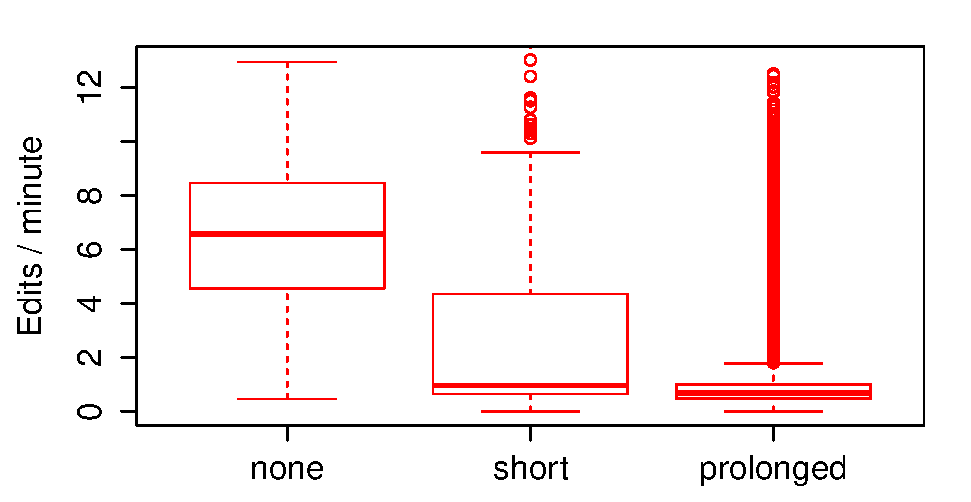
\includegraphics[width=\linewidth,clip=, angle=0]{figures/box_plot_range_edit}  
%\endminipage\hfill
%\minipage{0.33\textwidth}
%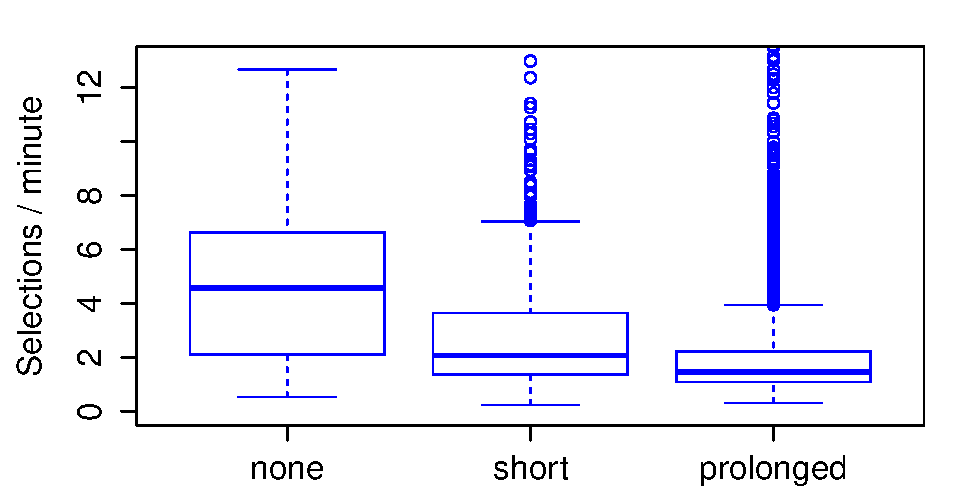
\includegraphics[width=\linewidth,clip=, angle=0]{figures/box_plot_range_sel}  
%\endminipage\hfill
%\minipage{0.33\textwidth}
%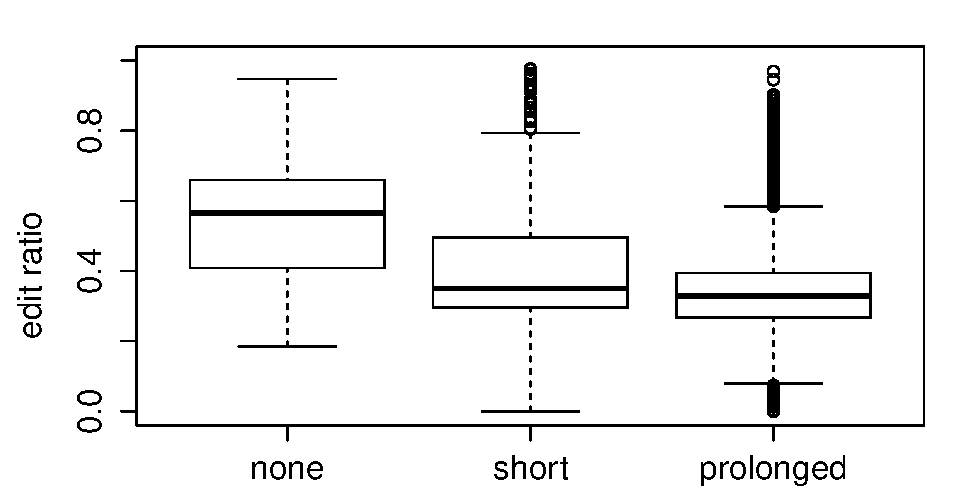
\includegraphics[width=\linewidth,clip=, angle=0]{figures/box_dur_ratio}
%\endminipage\hfill
%\end{tabular}
%\caption{Boxplots showing the relation between the number of edits and selections per minute, the edit ratio and interruption duration in Mylyn}
%\label{fig:box_dur_events}
%\end{figure}
%
%\begin{figure}[!ht]
%\centering
%\begin{tabular}{c}
%\minipage{0.33\textwidth}
%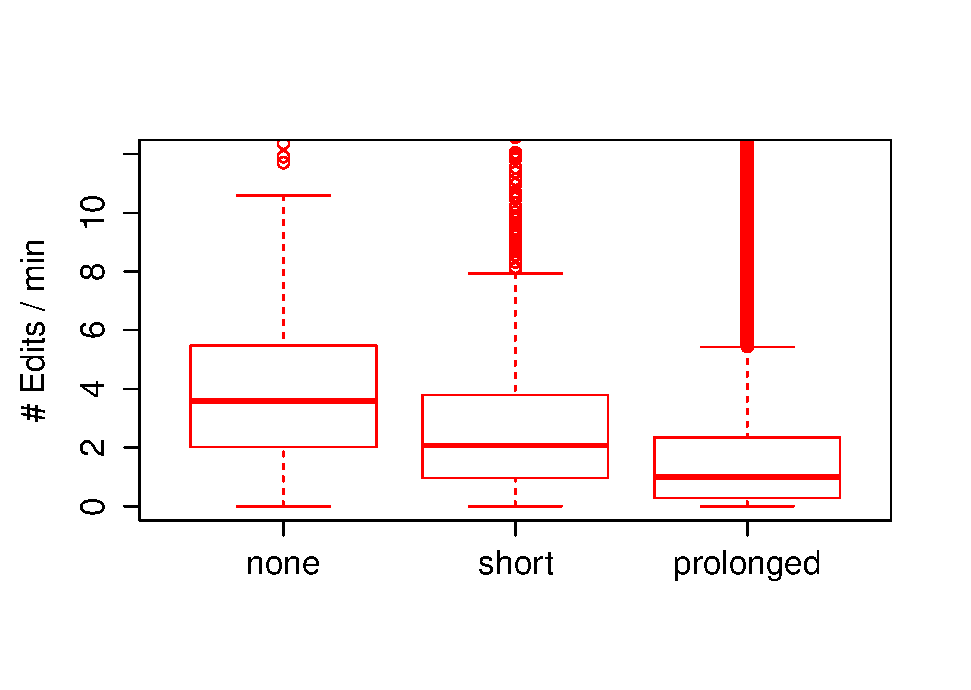
\includegraphics[width=\linewidth,clip=, angle=0]{figures/udc_box_plot_range_edit}  \\
%\endminipage\hfill
%\minipage{0.33\textwidth}
%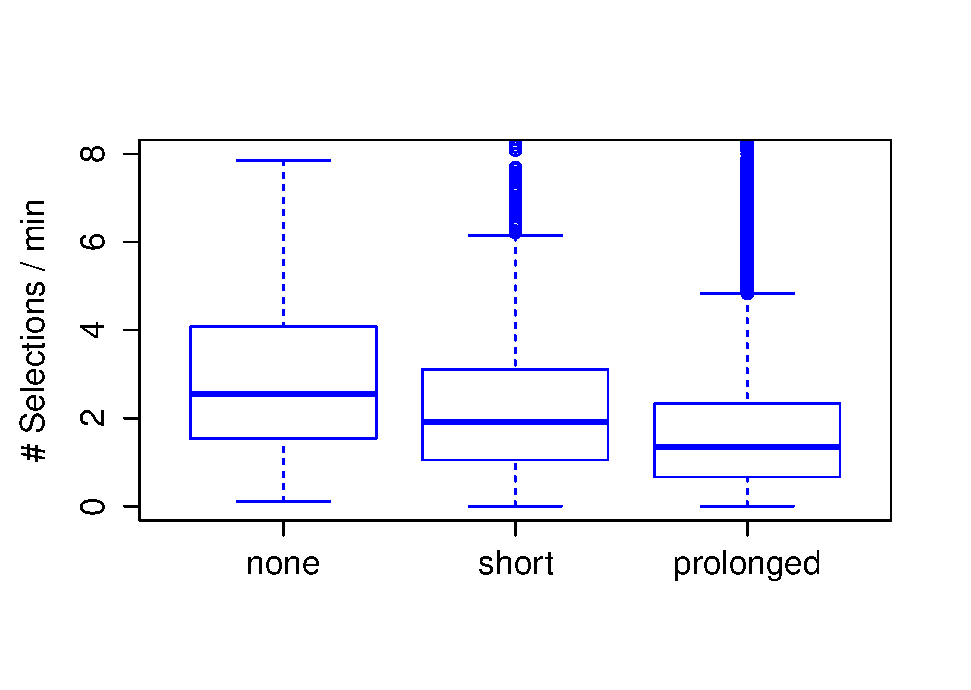
\includegraphics[width=\linewidth,clip=, angle=0]{figures/udc_box_plot_range_sel}  \\
%\endminipage\hfill
%\minipage{0.33\textwidth}
%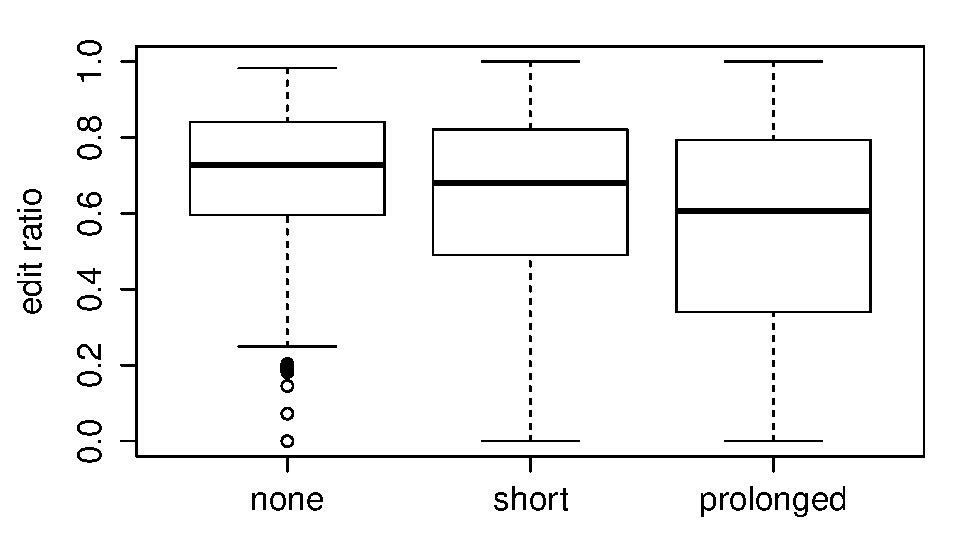
\includegraphics[width=\linewidth,clip=, angle=0]{figures/udc_box_dur_ratio} \\
%\endminipage\hfill
%\end{tabular}
%\caption{Boxplots showing the relation between the number of edits and selections per minute, the edit ratio and interruption duration in UDC}
%\label{fig:box_dur_events_udc}
%\end{figure}
%
%
%With Mylyn, as in the previous case, the differences are significant, and we used \textit{Cohen's d} to measure the practical significance of the means (Table \ref{tbl:p_value2}). We note that the effect size of the interruption duration over the number of edits per minute is very large. In selections, the effect is moderate for short interruptions, and large for prolonged interruptions.
%
%The effect size test results in the Table \ref{tbl:p_value2_udc} correspond to the results with UDC, and matches the previous observations (RQ1) on a less pronounced effect compared to the Mylyn dataset. The Cohen's \textit{d} test results tell us that we can label the effect from medium to large and the median values act accordingly to our observations in Mylyn. Therefore, we conclude that the relationship between user activity and interruptions could be adversely affected by interruptions of longer duration. 
%
%\begin{table}[ht!]
%\tiny
%\renewcommand{\arraystretch}{1.3}
%\caption{Effect size and statistical significance of the relationships between edits and selection per minute, edit ratio, and duration of interruptions in Mylyn} %, and editions and selections.}
%\label{tbl:p_value2}
%\centering
%\begin{tabular}{l | p{0.7cm} | p{1.9cm} | p{1.9cm} } 
%   & none & short &  prolonged  \\  
%  \hline
%  \multicolumn{4}{c}{\textbf{Edits}} \\
%  \hline
%  mean & 6.96 &	2.98 & 1.76 \\ 
%  % \cline{3-4} 
%  %t.test & $\hookrightarrow$& \multicolumn{2}{c}{$<$ 2.2e-16} \\
%   \cline{3-4} 
%  U-test & $\hookrightarrow$ & \multicolumn{2}{c}{$<$ 2.2e-16}  \\
%
%  \cline{3-4} 
%  Cohen's $d$ & $\hookrightarrow$	& \textbf{1.23} & \textbf{2.11}   \\
%  \hline
%  
%  
%  \multicolumn{4}{c}{\textbf{Selections}} \\
%  \hline 
%  mean & 5.20 &	3.33 & 2.47 \\ 
%  % \cline{3-4} 
%  %t.test & $\hookrightarrow$& 2.089e-08 & 8.175e-14 \\
%   \cline{3-4} 
%  U-test & $\hookrightarrow$ & 6.197e-13 & $<$ 2.2e-16 \\
%  
%  \cline{3-4} 
%  Cohen's $d$ & $\hookrightarrow$	& \textbf{0.63} & \textbf{1.24}  \\  
%  \hline
%  \multicolumn{4}{c}{\textbf{Edit ratio}} \\
%  \hline 
%  mean & 0.55 & 0.40 & 0.34\\ 
%%   \cline{3-4} 
%%  t.test & $\hookrightarrow$&  4.20E-12 & $<$ 2.2e-16 \\
%   \cline{3-4} 
%  U-test & $\hookrightarrow$ & 3.72e-14 & $<$ 2.2e-16  \\
%  \cline{3-4} 
%  Cohen's $d$ & $\hookrightarrow$ & \textbf{0.86} & \textbf{1.32}\\
%\hline
%
%\end{tabular}
%\end{table}
%
%\begin{table}[ht!]
%\tiny
%\renewcommand{\arraystretch}{1.3}
%\caption{Effect size and statistical significance of the relationships between edits and selection per minute, edit ratio, and duration of interruptions in UDC data} %, and editions and selections.}
%\label{tbl:p_value2_udc}
%\centering
%\begin{tabular}{l | p{0.7cm} | p{1.9cm} | p{1.9cm} } 
%   & none & short &  prolonged  \\  
%  \hline
%  \multicolumn{4}{c}{\textbf{Edits}} \\
%  \hline
%  mean & 3.97 &	2.75 & 1.79 \\ 
%  % \cline{3-4} 
%  %t.test & $\hookrightarrow$& \multicolumn{2}{c}{$<$ 2.2e-16} \\
%   \cline{3-4} 
%  U-test & $\hookrightarrow$ &  $<$ 2.6e-12 & $<$ 2.2e-16  \\
%
%  \cline{3-4} 
%  Cohen's $d$ & $\hookrightarrow$	& \textbf{0.48} & \textbf{0.89}   \\
%  \hline
%  
%  
%  \multicolumn{4}{c}{\textbf{Selections}} \\
%  \hline 
%  mean & 3.10 &	2.37 & 1.78 \\ 
%  % \cline{3-4} 
%  %t.test & $\hookrightarrow$& 2.089e-08 & 8.175e-14 \\
%   \cline{3-4} 
%  U-test & $\hookrightarrow$ & $<$ 4.3e-07& $<$ 2.2e-16  \\
%  
%  \cline{3-4} 
%  Cohen's $d$ & $\hookrightarrow$	& \textbf{0.34} & \textbf{0.68}  \\  
%  \hline
%  \multicolumn{4}{c}{\textbf{Edit ratio}} \\
%  \hline 
%  mean & 0.68 & 0.63 & 0.56\\ 
%%   \cline{3-4} 
%%  t.test & $\hookrightarrow$&  4.20E-12 & $<$ 2.2e-16 \\
%   \cline{3-4} 
%  U-test & $\hookrightarrow$ & 0.01003 & $<$ 4.019e-09  \\
%  \cline{3-4} 
%  Cohen's $d$ & $\hookrightarrow$ & \textbf{0.21} & \textbf{0.44}\\
%\hline
%
%\end{tabular}
%\end{table}
%
%Similar results occur when we look at the edit ratio (Figures \ref{fig:box_dur_events} and \ref{fig:box_dur_events_udc}): the edit ratio is smaller in sessions that have prolonged interruptions, compared to the ones that only have short interruptions. At the bottom of the effect size (Tables \ref{tbl:p_value2} and \ref{tbl:p_value2_udc}), we show the statistical and practical significance of these results. In Mylyn, we observe large effect sizes when comparing sessions who do not have interruptions with ones that do have, and larger effect sizes for sessions with at least one longer interruption.
%
%These findings seem to indicate that the inverse relationship between productivity and time of duration is more pronounced in session with at least one longer interruption. This agrees with the literature for information workers.

\section{RQ3: Local Relationships between Interruptions and Productivity}

The impact of work fragmentation could be more noticeable in the immediate minutes before and after an interruption occurs. On one hand, after an interruption the programmer carry out activities meant to recover the lost mental model, like reading the code, debugging, reading notes and cues, and more resumption strategies \cite{PR11}.

\RR{expand this paragraph, since a reviewer asks explicitely for that}
On the other hand, before the interruption there is a preparation phase when the interruption is imminent or expected. In this phase the programmer might leave notes or comments in the code to recover the context after the interruption \cite{PD10}. Also, when the interruption happened because of a problem found by the programmer, usually he tries to solve it by reading the code, using the debugger or reading comments in the control version tool; after this resources are depleted, the next option is to ask to teammates or other external resources \cite{LVD06}. The latest activities can represent an interruption of work.

In this research question we expect to see the effects on productivity around an interruption due to the activities previously described.


\subsection{Generic Sessions}

In order to better understand the relationship between work fragmentation and productivity, we need to delve deeper and perform local analyses of the development sessions. In the first step, we wanted to summarize how the activity of users is distributed over time in sessions which have no interruptions, short interruptions, and prolonged interruptions. For this, we created the following groups:
\begin{itemize}
	\item \textit{none}: the first group contains sessions with no interruptions.
	\item \textit{short}: the second group consists of sessions that only have short interruptions ($<$ 12 minutes of duration). 
	\item \textit{prolonged}: the third group consists of the remaining sessions, which have at least one prolonged interruption ($\geq$ 12 minutes of duration). 
\end{itemize} 

We performed this grouping in both Mylyn and UDC, obtaining the proportions shown in Table \ref{tbl:short_prol_int}. In both datasets the proportion of sessions with at least one long interruption is much larger than the rest, and there are a few sessions without interruptions.

\begin{table}[ht!]
	\small
	\renewcommand{\arraystretch}{1.3}
	\caption{Proportion of sessions with short interruptions, at least one prolonged interruptions and none} %separate the data in four percentages groups regarding the number of interruptions in each trace.}
	\label{tbl:short_prol_int}
	\centering
	\begin{tabular}{l | p{0.6cm} | p{0.6cm} | p{0.6cm}} 
		 & none & short & prolonged  \\  
		\hline 
		Mylyn &  2\% & 18\% & 80\% \\ 
		\hline  
		UDC &  1\% & 6\% & 93\%  \\  
	\end{tabular}
\end{table}

To summarize the development sessions, we have resized each time series to a single $size$, using local means. We have used $size = 10$, that is, dividing each session in 10 chunks of equal time, since because it yielded better global visualization (better uniformity) of the user interaction along a session. For each chunk, we choose the median value of edits and selections for each group, and compose one summary time series for each group; these are the time series displayed in Figure \ref{fig:bins_int}, for Mylyn, and Figure \ref{fig:bins_int_udc}, for UDC.

We observe that the median activity in sessions with interruptions is less than in sessions without interruptions, mainly in the edit frequency. Moreover, the edit frequency exceeds the selection frequency in sessions without interruptions. The opposite occurs in sessions with at least one interruption---and is more pronounced when there is at least one prolonged interruption---, where the code navigation tends to exceed the frequency of edits. These results agree with our earlier results. 

We also notice that the time series without interruptions have much more edits in the middle of the session than the others. This observation matches the hypothesis that developers need time to build their mental model for their task, and are less productive early in a session. This is similar to the edit lag in Parnin's study~\cite{PR11}: in sessions without interruptions, the edit lag is clearly visible at the start of the session. This behavior is not visible in sessions with interruptions; indeed, each session may have several edit lags (after each interruptions), and those would be equally distributed over the entire duration of the session, resulting in the ``flat lines" that we see for these sessions.

These results support our previous observations at a finer level, and corroborate the literature saying that time is needed to start or get back on task. Also, we observe the same conclusions in the results with UDC, but there are some subtle differences. For instance, the distance between edit and selections in every chunk is shorter than the results with Mylyn, and during sessions with short interruptions the selections start being greater that the editions, but around the middle of the session the latest slightly recover, and finish below the selections again at the end of the session.

%Therefore, with this result, we also infer that the presence of interruptions in a programming task could reduce the user interaction with the program. \\

%Another way to understand the effect of the interruptions in a programming task, was building global representations of the user activity e have considered three global representations for three groups of traces: the first trace represents to the traces without interruptions, the second to the traces that only  have short interruptions and the third to the traces that have at less one prolonged interruption. Then, 

\begin{figure}[!ht]
\centering
\begin{tabular}{c}
\minipage{0.33\textwidth}
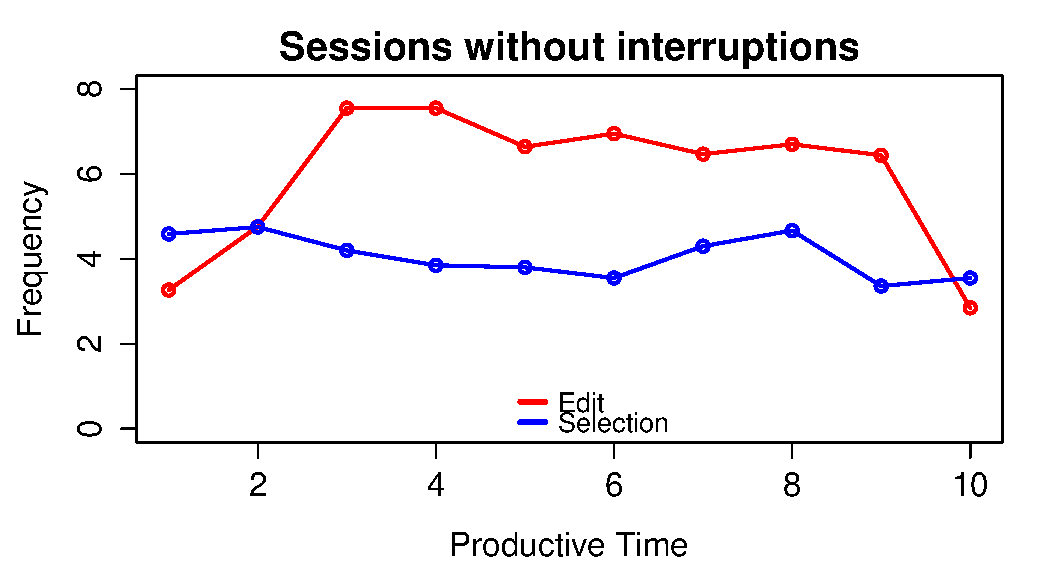
\includegraphics[width=\linewidth,clip=, angle=0]{figures/without_int_med} 
\endminipage\hfill
\minipage{0.33\textwidth}
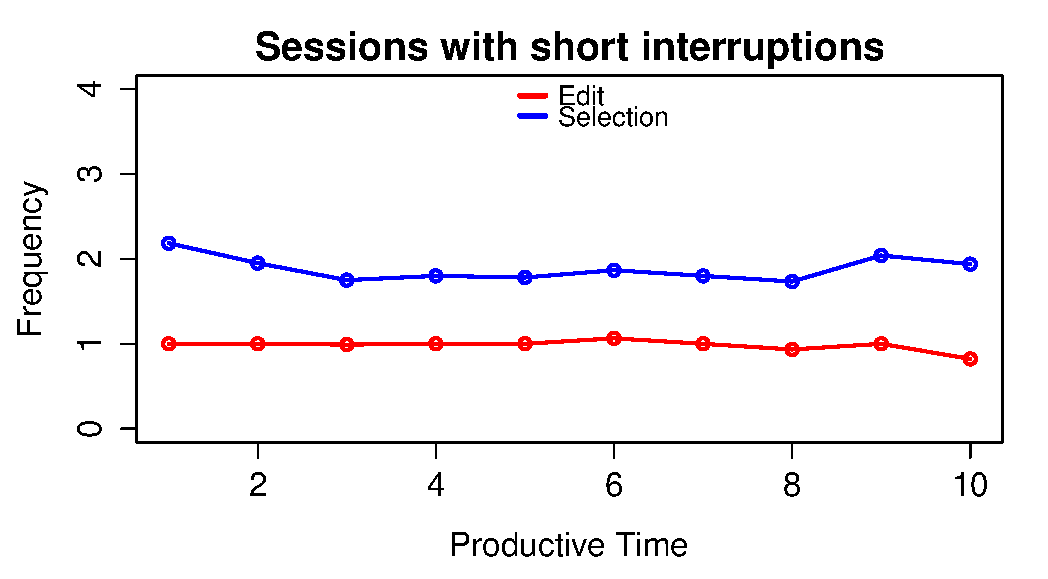
\includegraphics[width=\linewidth,clip=, angle=0]{figures/with_int1_med} 
\endminipage\hfill
\minipage{0.33\textwidth}
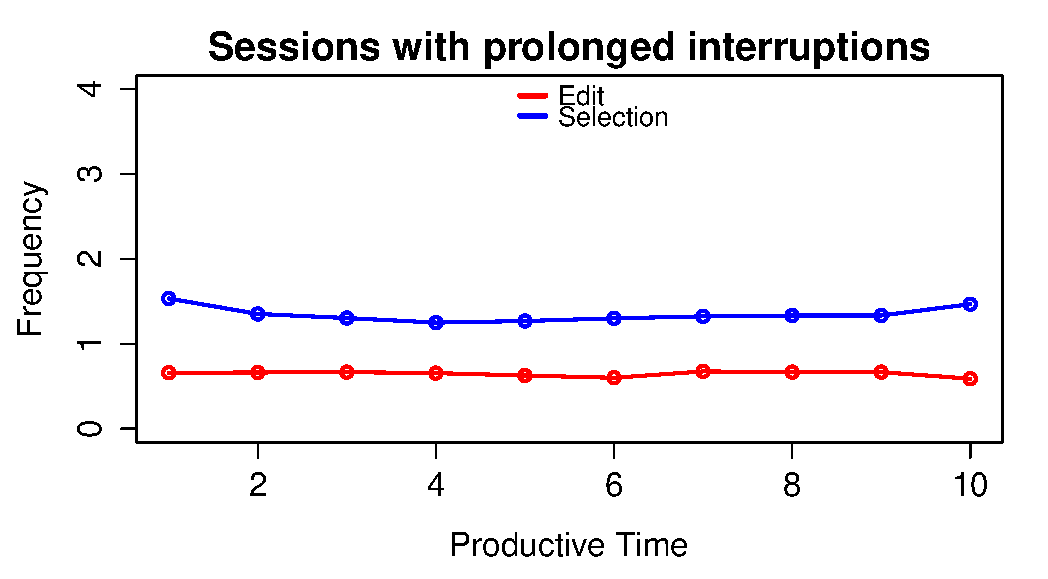
\includegraphics[width=\linewidth,clip=, angle=0]{figures/with_int2_med} 
\endminipage\hfill
\end{tabular}
\caption{Global representation of a session in Mylyn, with: no interruptions (left); only short interruptions (middle); and at least one prolonged interruption (right). }
\label{fig:bins_int}
\end{figure}

\begin{figure}[!ht]
	\centering
	\begin{tabular}{c}
		\minipage{0.33\textwidth}
		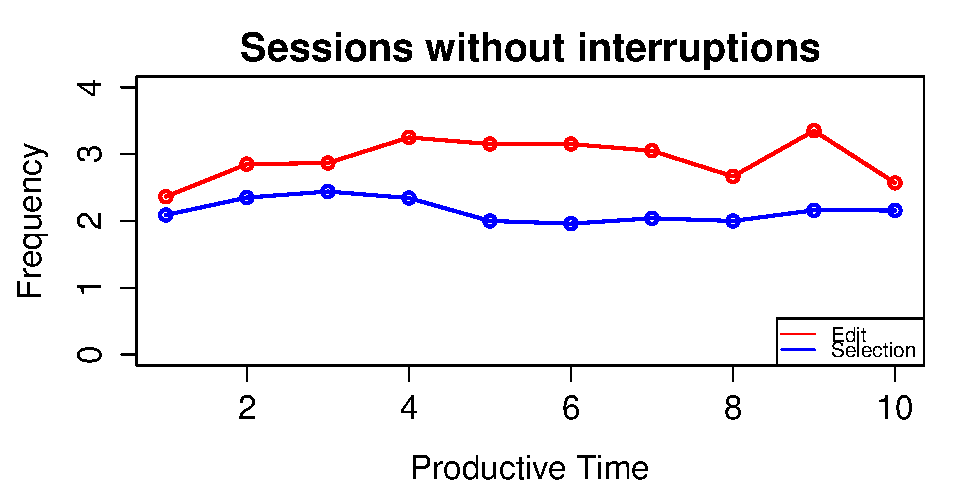
\includegraphics[width=\linewidth,clip=, angle=0]{figures/udc_without_int_med} \\
		\endminipage\hfill
		\minipage{0.33\textwidth}
		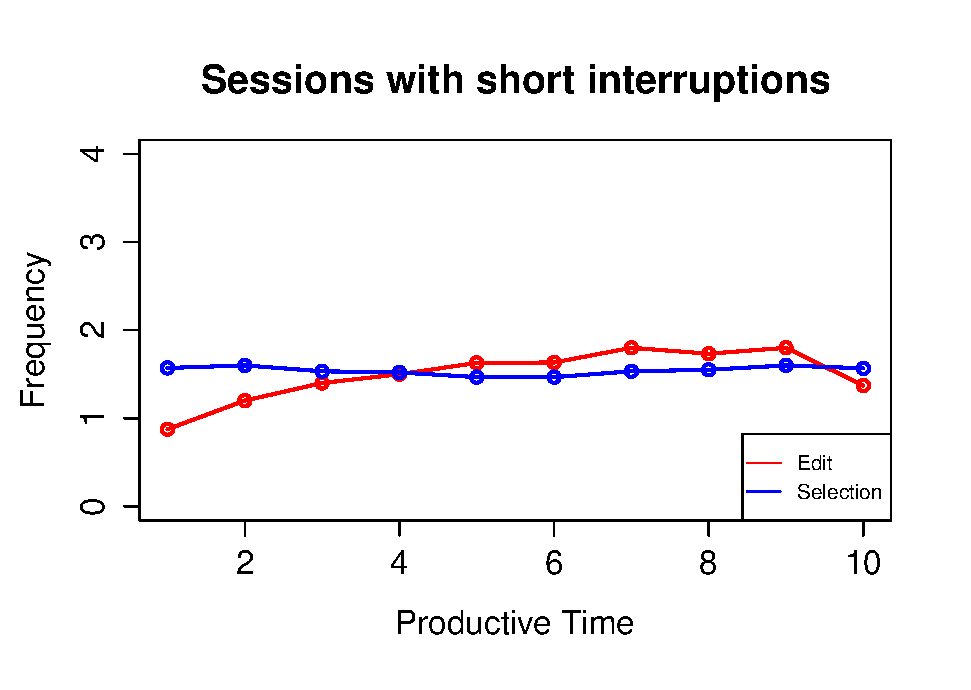
\includegraphics[width=\linewidth,clip=, angle=0]{figures/udc_with_int1_med} \\
		\endminipage\hfill
		\minipage{0.33\textwidth}
		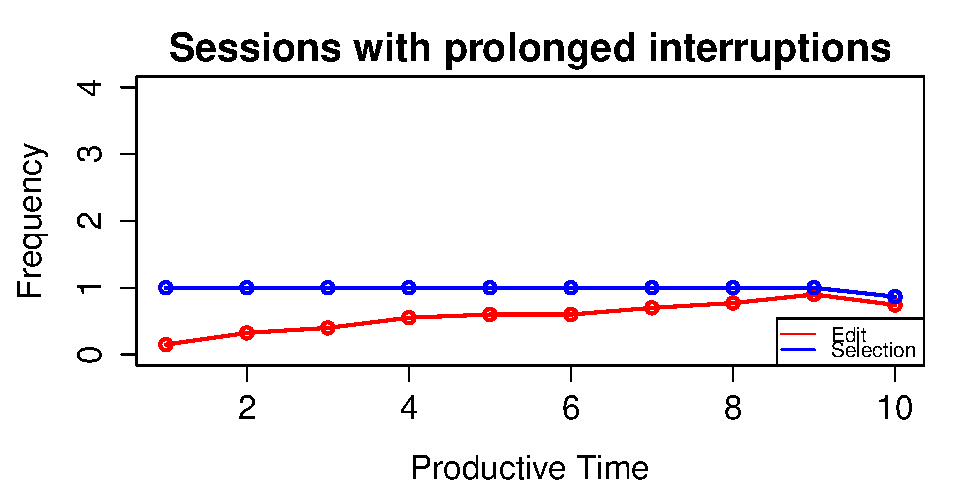
\includegraphics[width=\linewidth,clip=, angle=0]{figures/udc_with_int2_med} \\
		\endminipage\hfill
	\end{tabular}
	\caption{Global representation of a session in UDC, with: no interruptions (left); only short interruptions (middle); and at least one prolonged interruption (right). }
	\label{fig:bins_int_udc}
\end{figure}



\subsection{Local Analysis}

Having presented the global effect of the interruptions over the user productivity, we now focus on the local activity before and after interruptions. We take a maximum real time interval of 30 minutes around each detected interruption, obtaining a set of 26,988 time series subsequences in Mylyn and 97,984 in UDC. Then, we compute the median of all these subsequences as a generic local representation (Figure \ref{fig:all_ints}). We also plot with dashed lines the median values of edits and selections per minute in the sessions with interruptions in order to give more context to the observed values.
%where another interruption  should not have been found. 
Below we describe some observations:
\begin{itemize}
\item \textit{In the center,} we find the interruption point. There is clearly a negative effect on the time series, as the area before and after the interruption is the area with the lowest activity. The activity is well below the median activity of time series with interruptions, showing that the effect is indeed more pronounced near interruptions. This happens in Mylyn and UDC.

\item \textit{On the right,} the trend of the time series increases steadily. We hypothesize that the programmer is immersing again into the programming task, increasing progressively the activity as represented by the number of edits and selections. In Mylyn it reaches the median activity (in average) 12 to 18 minutes after the interruption, while in UDC it is around 6 to 12 minutes. It then rises further than the session median, which is not surprising, as we expect higher than median activity further away from interruptions.

%We called \textit{recuperation time} the first intersect point between edition and navigation. In this sense, the  average recuperation time of an interruption occurs in the minute 12. 
\item \textit{On the left,} we observe that the number of events near the interruption also goes down well below the median value. This might be because of two reasons: the programmer could have found a problem while coding, who at first will try to solve it by reading the code, switching out from the IDE, navigating the call stack and debugging, before going to ask another teammate according to LaToza et al. \cite{LVD06}; this set of actions end up with an interruption and reduce the observed activity within the IDE. Also, when the interruption is imminent or expected, the programmer make use of different suspension strategies like writing physical notes, making a mental note or leaving a reminder cue on the code or window, as mentioned by Parnin and DeLine \cite{PD10}. These activities reduce the activity before the gap and they are seen in the interaction data mostly as selection events. The latest can be better visualized in Figure \ref{fig:all_ints} with the UDC data as a significant decrease of edit events, being below the selection events approximately 10 minutes before the interruption.
%\item \textit{On the left,} we observe that the number of events near the interruption also goes down well below the median value. This is because work fragmentation is not only due to interruptions: programmers may for instance switch away from the IDE to look up information on the web or request it from other programmers. They are likely to do so because they are stuck, which would manifest itself by lower activity before the activity gap. We investigate this further below.

%This is more surprising, as we expected the activity to drop mostly after the interruption rather than before. A possible explanation is that their are several causes for inactivity
\end{itemize}


\begin{figure}[!ht]
\centering
\begin{tabular}{c}
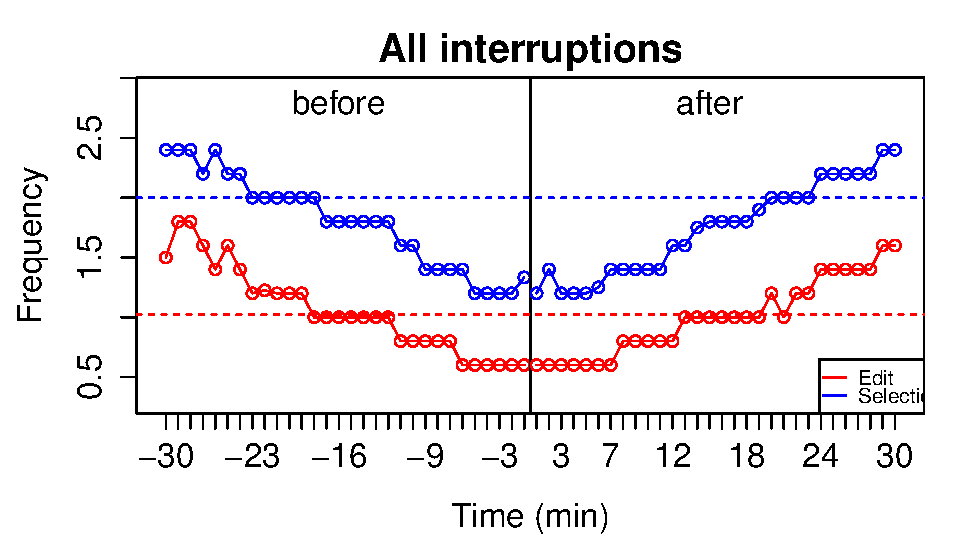
\includegraphics[width=0.6\linewidth,clip=, angle=0]{figures/all_ints} \\
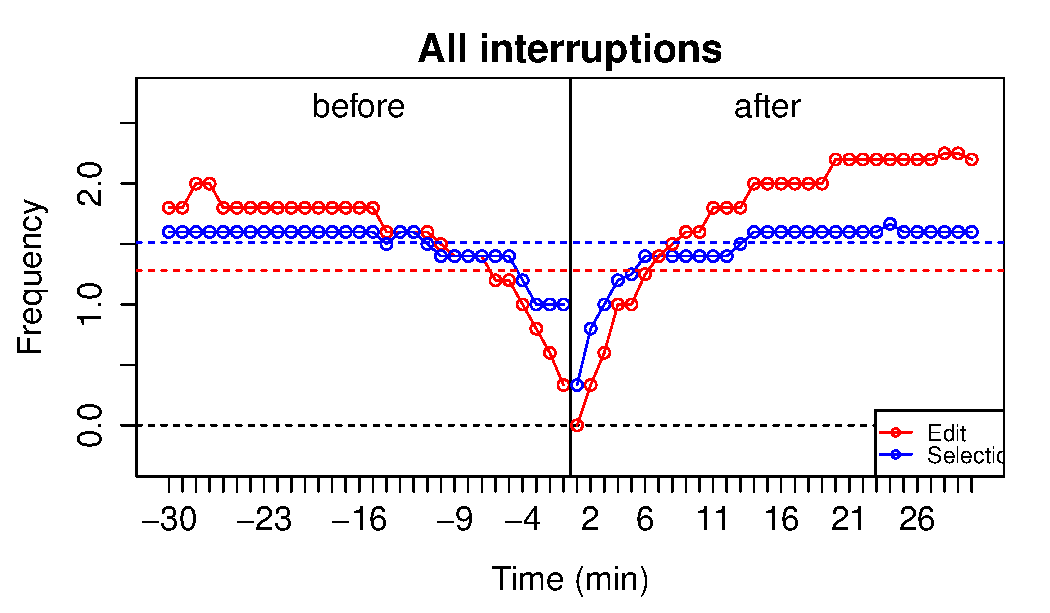
\includegraphics[width=0.6\linewidth,clip=, angle=0]{figures/udc_all_ints_2} 
\end{tabular}
\caption{Local effect of an interruption in the user activity for Mylyn (top) and UDC (bottom)}
\label{fig:all_ints}
\end{figure}
%
%\begin{figure}[!ht]
%	\centering
%	\begin{tabular}{c}
%		
%	\end{tabular}
%	\caption{Local effect of an interruption in the user activity.}
%	\label{fig:all_ints_udc}
%\end{figure}


We investigated whether the drop in activity local to interruptions was also accompanied by a drop in the edit ratio. We computed the edit ratio over slices of 5 minutes before and after each interruption (smaller intervals would be too sensitive to noise). The boxplots in Figure \ref{fig:ratio_all} show that the edit ratio drops slightly the closer we are to an interruption. The effect is small, but significant (see Table \ref{tbl:ratio_all}). As a reference, the mean edit ratio for sessions with short interruptions is 0.4, so the edit ratio close to the interruptions are clearly lower in the 5 to 10 minutes around an interruption. This matches the observations Parnin made with the edit lag \cite{PR11}.

\begin{figure}[!ht]
\centering
\begin{tabular}{c}
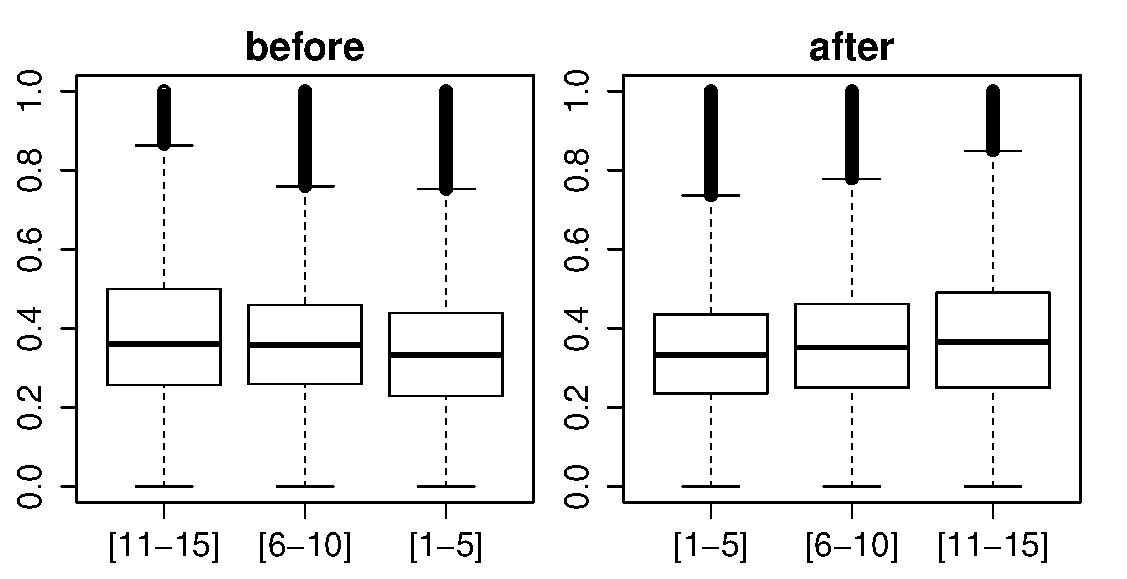
\includegraphics[width=0.5\linewidth,clip=, angle=0]{figures/ratio_all} 
\end{tabular}
\caption{Ratio of edits around the interruption. }
\label{fig:ratio_all}
\end{figure}


\begin{table}[ht!]
\tiny
\renewcommand{\arraystretch}{1.3}
\caption{Effect size of the ratio of edits around the interruption.}
\label{tbl:ratio_all}
\centering
\begin{tabular}{l | p{0.7cm} | p{1.9cm} | p{1.9cm} } 
   & [1-5] & [6-10] & [11-15] \\  
  \hline
  \multicolumn{4}{c}{\textbf{before}} \\
  \hline
  mean & 0.34 &	0.37 &	0.39 \\ 
   \cline{3-4} 
  U-test & $\hookrightarrow$ & \multicolumn{2}{c}{$<$ 2.2e-16}  \\

  \cline{3-4} 
  Cohen's $d$ & $\hookrightarrow$	& \textbf{0.16} & \textbf{0.24}   \\
  \hline
  
  
  \multicolumn{4}{c}{\textbf{after}} \\
  \hline 
  mean & 0.34 &	0.37 &	0.39 \\ 
   \cline{3-4} 
  U-test & $\hookrightarrow$ & 5.67e-16 & $<$ 2.2e-16 \\  
  \cline{3-4} 
  Cohen's $d$ & $\hookrightarrow$	& \textbf{0.14} & \textbf{0.22}  \\  
\end{tabular}
\end{table}

\subsection{Patterns of Interruptions}
Given the overall activity pattern we noticed in the local analysis, we hypothesize that there are several kinds of interruptions, matching the scenarios observed in the literature: actual interruptions distracting the programmer from the task at hand, and switching tasks in case of being stuck in the current task.

We hence looked for patterns in the interruptions.  After applying clustering techniques over all the subsequences, we always found the formation of three recurrent patterns that show different effects of the interruption: neutral, positive and negative. The clustering was performed with the  K-Mediods~\cite{AMP97} technique, the Silhouette metric~\cite{RP87} to interpret and evaluate the results, the Dynamic Time Warping~\cite{KE05} as distance measure, and feature extraction techniques to reduce the dimensionality.  For this reason, we classified empirically each interruption by its local effect. 

We did so by computing Cohen's $d$ on the quantity of edits before and after the interruption. To obtain a significant effect, we need the presence of activity both before and after. Not all the interruptions meet this criteria however: some are located close to the start or the end of a session, or too close to another interruption.  In total, 53\% of the interruptions had 30 minutes before and after the interruption and were selected for the analysis.  The remaining 47\% of the interruptions can not be used on this analysis due to the lack of time around them. %We used the Algorithm \ref{alg:local_effect} for the classification, and the 
Table \ref{tbl:local_effect} shows the applied thresholds and the results, accompanied with a typical example of an interruption in each category. This local analysis shows that there are indeed three well-defined groups of interruptions, with the two largest of them having clear effects on the activity in the session.



%\begin{algorithm}[t]
 %\begin{algorithmic}[1]
   %\Require (Before edits  $B$, After edits $A$)  
   %\State $effect=`` "$
	%
	%\If{$\frac{|\bar{A} - \bar{B}|}{\sigma(A,B)} \leq 0.2$}
		%\State $effect=``neutral"$
	%\ElsIf{$\bar{A} \geq \bar{B}$}
		%\State $effect=``positive"$
	%\Else
		%\State $effect=``negative"$
    %\EndIf
    %
%\State \Return $effect$
 %\end{algorithmic} 
 %\caption{Compute the Local Effect}
 %\label{alg:local_effect}
%\end{algorithm}		

\begin{table}[ht!]
\caption{Local Effect of Interruption. }
\label{tbl:local_effect}
\centering
\begin{tabular}{p{5cm} | c | c}
effect & pattern in Mylyn & pattern in UDC \\
\hline
\textit{negative}: when the frequency of edit events decreases after the interruption (Cohen's $d < -0.2$)
	& 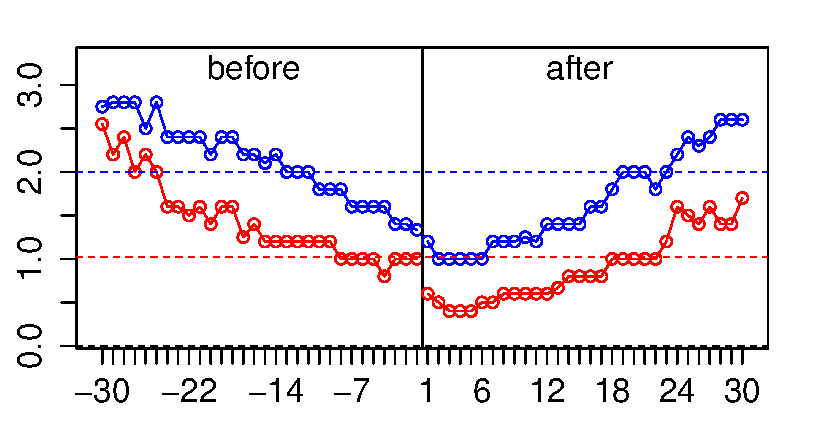
\includegraphics[valign=m,scale=0.3]{figures/neg_ints}
	& 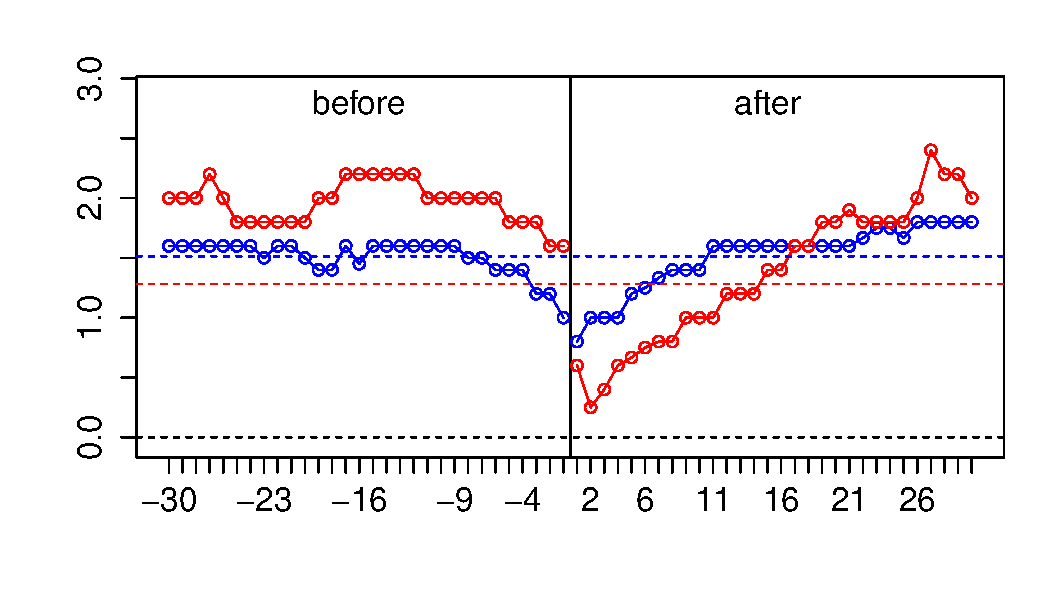
\includegraphics[valign=m,scale=0.24]{figures/udc_neg_ints_2}  \\
\textit{positive}: when the frequency of edit events increases after the interruption (Cohen's $d > 0.2$)
	& 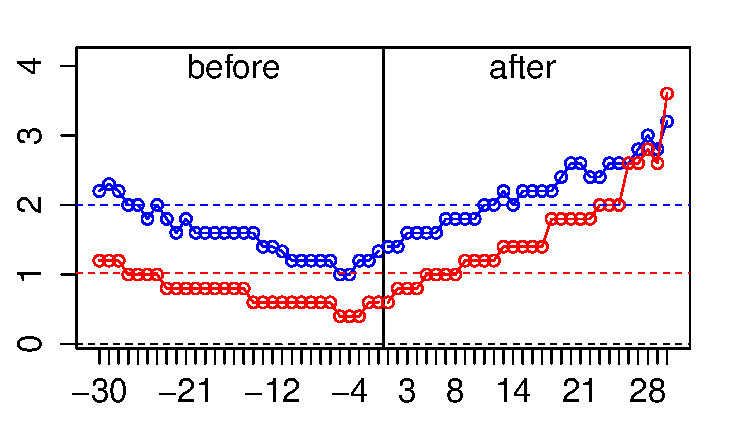
\includegraphics[valign=m,scale=0.3]{figures/pos_ints}
	& 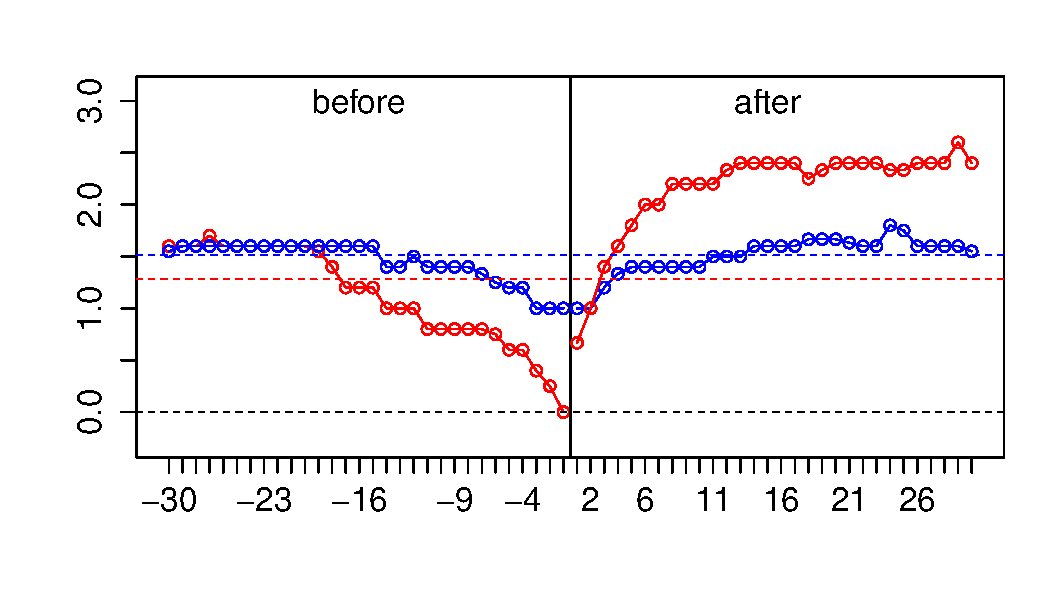
\includegraphics[valign=m,scale=0.24]{figures/udc_pos_ints_2} \\
\textit{neutral}: when there is no well defined effect before or after the interruption ($abs(d) <= 0.2$)
	& 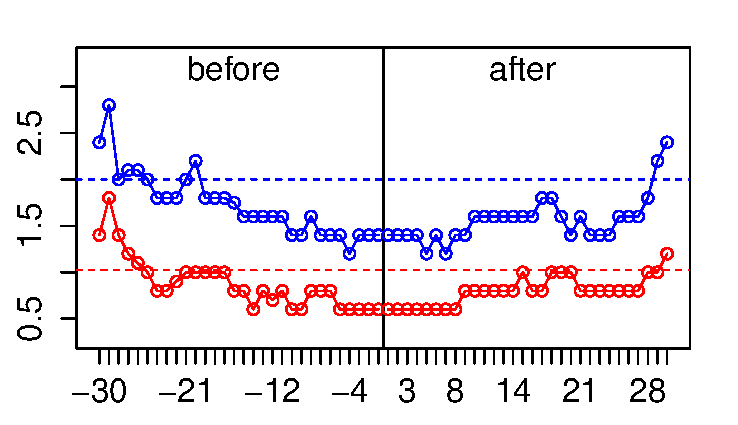
\includegraphics[valign=m,scale=0.3]{figures/neu_ints} 
	& 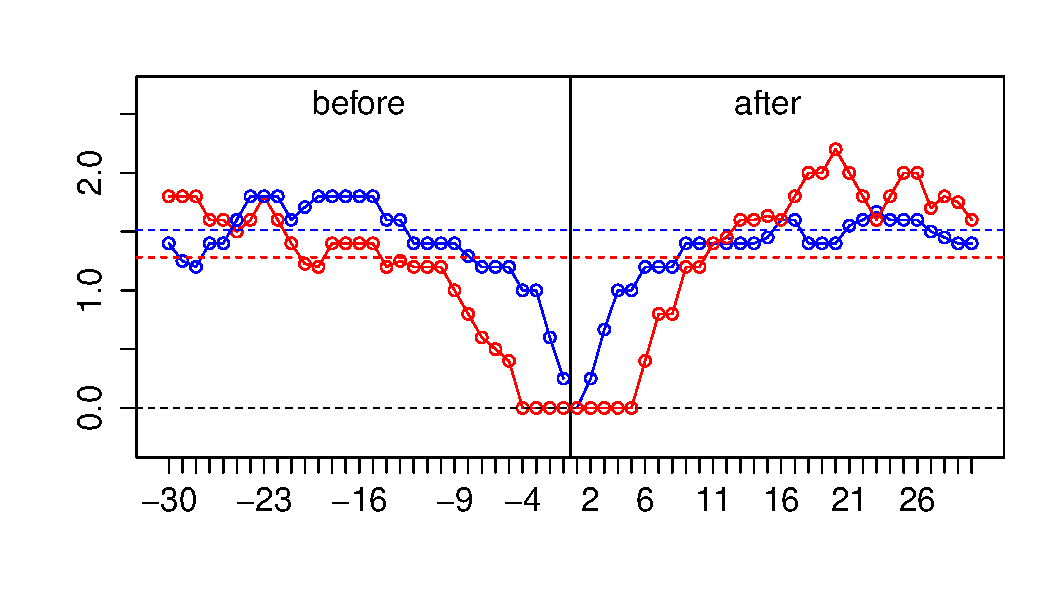
\includegraphics[valign=m,scale=0.24]{figures/udc_neu_ints_2} 
\end{tabular}
\end{table}

The results in UDC indicate that after a positive interruption, both metrics tend to increase at a high rhythm until reaching the global average value. The edits per minute recover quickly (approximately 5 minutes after the interruption), but the selections per minute take a little longer to reach the global average, and this metric tend to be below the average for an extended period. It is important to notice that before the interruption happens the editions per minute metric is below the average for approximately 16 minutes prior to the interruption.

In contrast, when facing the effects of a negative interruption the metrics take longer to reach the median. On the contrary to facing a positive interruption, the editions per minute metric is below the selections per minute, and the former takes longer than the latter to reach the average value. Also, the editions per minute metric is above the average for the 30 minutes before the interruption. 

In general, the effect of positive and negative interruptions is the inverse. The editions per minute describes better the effect and the selections do not show a major change. There is not a clear pattern during a neutral interruption.

Finally, we briefly report on the edit ratios for positive and negative interruptions (see Figure~\ref{fig:ratio_rest}). We see distinct patterns as well: positive interruptions have a higher edit ratio after the interruption (in accordance with the hypothesis of a more efficient activity after having looked for missing information), while negative interruptions have a lower edit ratio after the interruption (in accordance with the hypothesis that the programmer may be rebuilding his context after an unwanted task switch).

\begin{figure}[!ht]
\centering
\begin{tabular}{c}
\minipage{0.5\textwidth}
\begin{center}
{Positive Effect}
\end{center} 
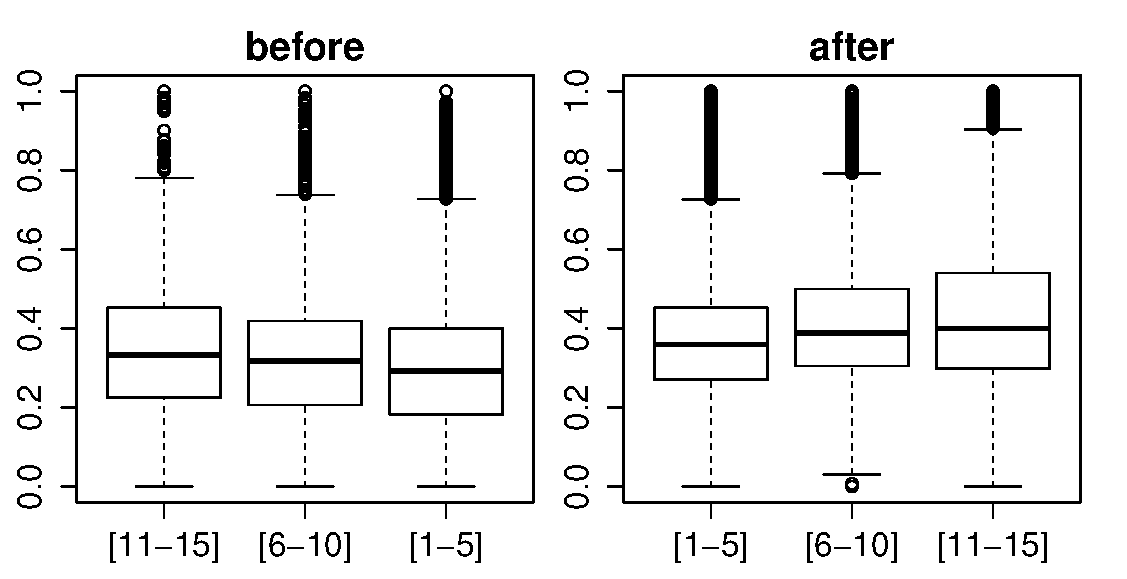
\includegraphics[width=\linewidth,clip=, angle=0]{figures/ratio_pos} \\ 

\endminipage\hfill
\minipage{0.5\textwidth}
\begin{center}
Negative Effect
\end{center}

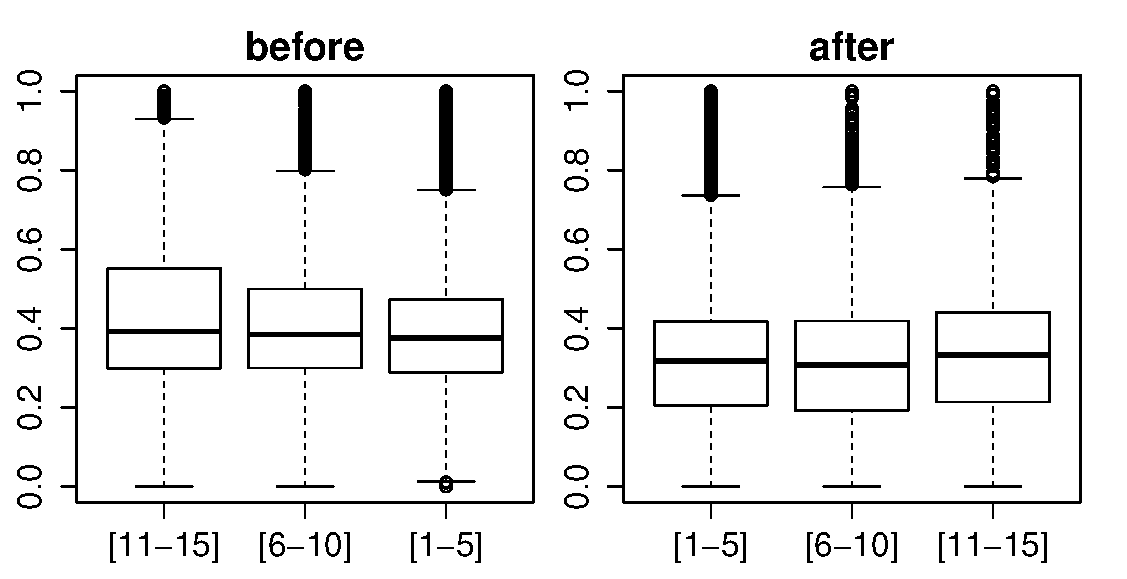
\includegraphics[width=\linewidth,clip=, angle=0]{figures/ratio_neg} \\
\endminipage\hfill
\end{tabular}
\caption{Ratio of edits for positive and negative local effect. }
\label{fig:ratio_rest}
\end{figure}






%\section{Results of RQ1, RQ2, and RQ3 on UDC}
%
%\subsection{RQ1: Relationship between interruptions and productivity}
%We used the same metrics to investigate whether we could observe a similar behavior with the new dataset. To analyze the effects of interruptions on productivity we divided the sessions according to the quantiles of the distribution of the number of interruptions they hold. We obtained slightly different results to Mylyn, and consequently we changed the thresholds used to classify the sessions by the number of interruptions. Although the change is small, the distribution of the number of interruptions differs and indicates that on UDC the sessions contains less interruptions. It is important to reflect this change on the results and compare them against the results with Mylyn on fair ground, as the same procedure was done with that dataset. The new thresholds are shown in the Table \ref{tbl:quartil_int_udc} and were used to classify every session according to the number of interruptions that it has.
%
%\begin{table}[ht!]
%\tiny
%\renewcommand{\arraystretch}{1.3}
%\caption{Thresholds used to group sessions based on their number of interruptions for the UDC data} %separate the data in four percentages groups regarding the number of interruptions in each trace.}
%\label{tbl:quartil_int_udc}
%\centering
%\begin{tabular}{l | p{0.6cm} | p{0.6cm} | p{0.6cm}} 
%     & $25\%$ & $50\%$ & $75\%$ \\  
%  \hline 
%  quartile &  2 & 4 & 7  \\   
%\end{tabular}
%\end{table}
%
%For every session, we calculated the number of editions and selections per minute, and the edit ratio. The boxplots in the Figure \ref{fig:box_int_events_udc} show a similar pattern in comparison with the results with Mylyn. When facing zero interruptions the editions and selections per minute are greater than with one or more interruptions, and as more interruptions occur this metrics gradually decrease.
%
%
%
%The edit ratio behaves similarly in comparison with the data on Mylyn, where the median changes accordingly with the number of interruptions, decreasing when there are more and reaching the maximum when there are none. An important difference is that the effect overall appears to be less pronounced in UDC and we can see it on the effect size tests shown in the Table \ref{tbl:p_value_udc}. Most of the observed effects are medium, while in the Mylyn datasets the effects were large. Note despite the differences in effect sizes, the differences are still significant.
%
%
%
%\subsection{RQ2: Relationship between duration of interruptions and productivity}
%The next analysis is on the effects of the size of the interruptions, considering short and prolonged interruptions.
%\begin{itemize}
%\item \textit{short}: as with Mylyn we considered those sessions that have only short interruptions ($<$ 12 minutes of duration). They constitute 6\% of the total.
%\item \textit{prolonged}: this group of sessions have at least one prolonged interruption ($\geq$ 12 minutes of duration). They constitute 93\% of the total.
%\item \textit{none}: this group of sessions have no interruptions. They constitute 1\% of the total.
%\end{itemize} 
%
%\begin{figure}[!ht]
%\centering
%\begin{tabular}{c}
%\minipage{0.33\textwidth}
%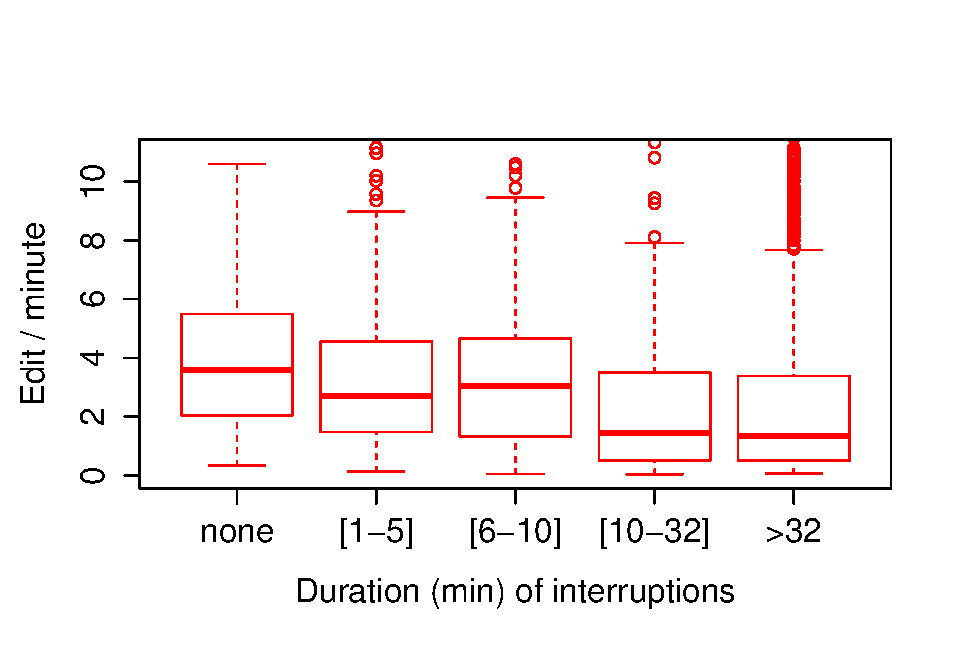
\includegraphics[width=\linewidth,clip=, angle=0]{figures/udc_box_plot_range_edit_2}  \\
%\endminipage\hfill
%\minipage{0.33\textwidth}
%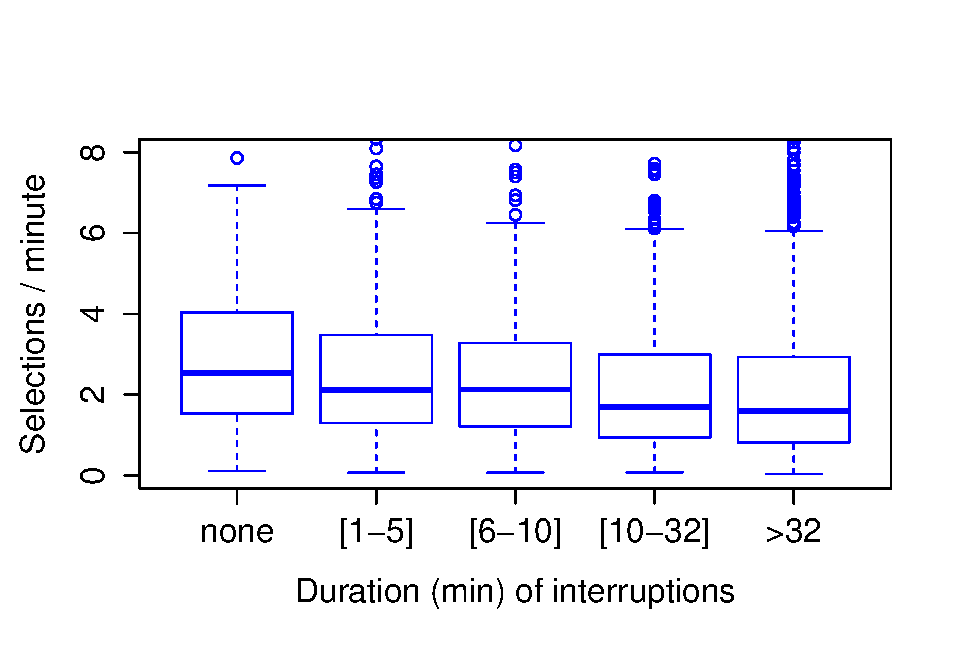
\includegraphics[width=\linewidth,clip=, angle=0]{figures/udc_box_plot_range_sel_2}  \\
%\endminipage\hfill
%\minipage{0.33\textwidth}
%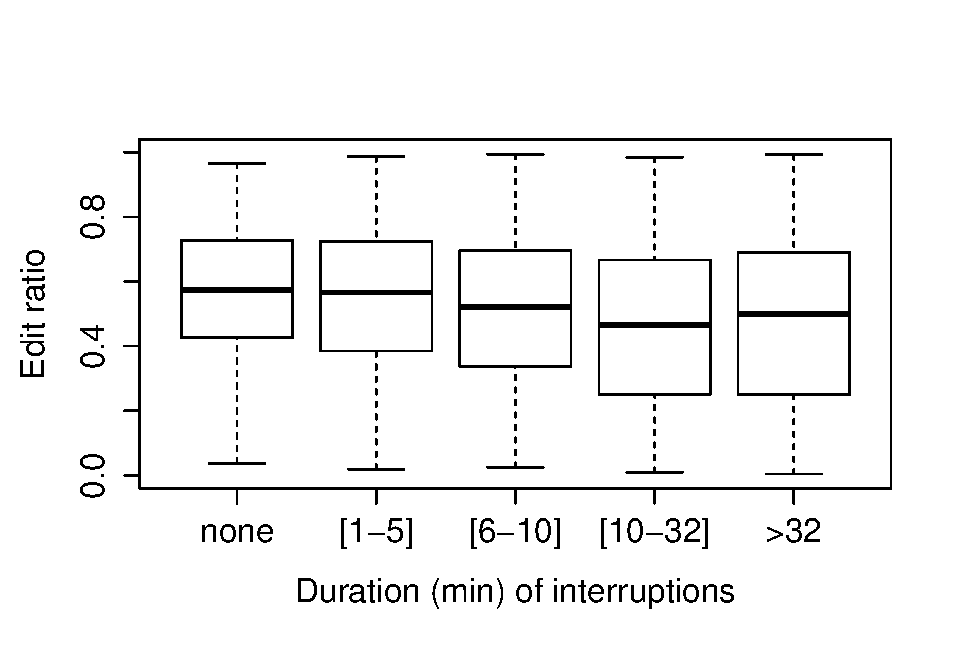
\includegraphics[width=\linewidth,clip=, angle=0]{figures/udc_box_dur_ratio_2} \\
%\endminipage\hfill
%\end{tabular}
%\caption{Boxplots showing the relation between the number of edits and selections per minute, the edit ratio and interruption duration}
%\label{fig:box_dur_events_udc}
%\end{figure}
%
%Again the hypothesis holds on UDC data as it did with Mylyn. We can see on the Figure \ref{fig:box_dur_events_udc} that with short interruptions the metrics are greater than when facing at least a prolonged one, for more time is needed to recover after a long interruption. 
%\begin{table}[ht!]
%\tiny
%\renewcommand{\arraystretch}{1.3}
%\caption{Effect size and statistical significance of the relationships between edits and selection per minute, edit ratio, and duration of interruptions on UDC data} %, and editions and selections.}
%\label{tbl:p_value2_udc}
%\centering
%\begin{tabular}{l | p{0.7cm} | p{1.9cm} | p{1.9cm} } 
%   & none & short &  prolonged  \\  
%  \hline
%  \multicolumn{4}{c}{\textbf{Edits}} \\
%  \hline
%  mean & 3.97 &	2.75 & 1.79 \\ 
%  % \cline{3-4} 
%  %t.test & $\hookrightarrow$& \multicolumn{2}{c}{$<$ 2.2e-16} \\
%   \cline{3-4} 
%  U-test & $\hookrightarrow$ &  $<$ 2.6e-12 & $<$ 2.2e-16  \\
%
%  \cline{3-4} 
%  Cohen's $d$ & $\hookrightarrow$	& \textbf{0.48} & \textbf{0.89}   \\
%  \hline
%  
%  
%  \multicolumn{4}{c}{\textbf{Selections}} \\
%  \hline 
%  mean & 3.10 &	2.37 & 1.78 \\ 
%  % \cline{3-4} 
%  %t.test & $\hookrightarrow$& 2.089e-08 & 8.175e-14 \\
%   \cline{3-4} 
%  U-test & $\hookrightarrow$ & $<$ 4.3e-07& $<$ 2.2e-16  \\
%  
%  \cline{3-4} 
%  Cohen's $d$ & $\hookrightarrow$	& \textbf{0.34} & \textbf{0.68}  \\  
%  \hline
%  \multicolumn{4}{c}{\textbf{Edit ratio}} \\
%  \hline 
%  mean & 0.68 & 0.63 & 0.56\\ 
%%   \cline{3-4} 
%%  t.test & $\hookrightarrow$&  4.20E-12 & $<$ 2.2e-16 \\
%   \cline{3-4} 
%  U-test & $\hookrightarrow$ & 0.01003 & $<$ 4.019e-09  \\
%  \cline{3-4} 
%  Cohen's $d$ & $\hookrightarrow$ & \textit{0.21} & \textit{0.44}\\
%\hline
%
%\end{tabular}
%\end{table}
%The effect size test results in the Table \ref{tbl:p_value2_udc} matches the previous observations on a less pronounced effect compared to the Mylyn dataset. The Cohen's \textit{d} test results tell us that we can label the effect from medium to large and the median values act accordingly to our hypothesis and conclusions with Mylyn.
%
%\subsection{RQ3: Local relationships between interruptions and productivity}
%The sessions with UDC went through the same process of transformation into 10 chunks of equal time. The results on the Figure \ref{fig:bins_int_udc} shows similar (but not identical) patterns compared to the ones we observed in Mylyn.
%
%
% 
%The median of editions and selections per minute are greater in sessions without interruptions, and the editions are more common than selections. Sessions with only short interruptions show a level of edit activity similar to selection activity overall, but with a tendency to rise overtime (except a drop in the last segment). When facing at least one prolonged interruption we can see the metrics drop in comparison with short interruptions and the selections are now more frequent than the edit events. This agrees with the results with Mylyn on this point. 
%
%As for the observation that activity was overall higher in the middle of the session we do see this for sessions without interruptions. For sessions with interruptions, selection activity appears to be constant over time, while edit activity appears to rise over time with a slight drop at the end.
%
%On a local analysis around the interruptions, we can see a similar interesting behavior of the edition and selections metrics as we observed with Mylyn. In the Figure \ref{fig:all_ints_udc} we show the frequency of editions and selections around the interruptions, specifically 30 minutes before and after. We observed that close to the interruption the frequency of editions and selections drastically drop, and in a radius of around 10 minutes both metrics are below the overall median. This phenomenon is also visible on the same version of this plot with Mylyn, agreeing that the activity of programming gradually decreases before the interruption and takes several minutes to restore the intensity of work above the median. Similarly than for Mylyn, we can see that the edits pass below the selections events near the interruption. %In contrast to the overall trend, the overall effect appears to be more drastic for UDC data this time.
%
%
%
%After this, we separated the interruptions in three categories: those with positive effects afterwards, those a with negative effect and those with no clear effect. Both positive and negative interruptions have a proportion of $44\%$ each of all the interruptions, and the neutrals stand with the $12\%$, and they are similar to the proportions on Mylyn. The results are in the Table \ref{tbl:local_effect_udc}. 
%
%\begin{table}[ht!]
%\caption{Local Effect of Interruption. }
%\label{tbl:local_effect_udc}
%\centering
%\begin{tabular}{p{4cm} | c}
%effect & pattern \\
%\hline
%\textit{negative} (44\%): when the frequency of edit events decreases after the interruption
%	& 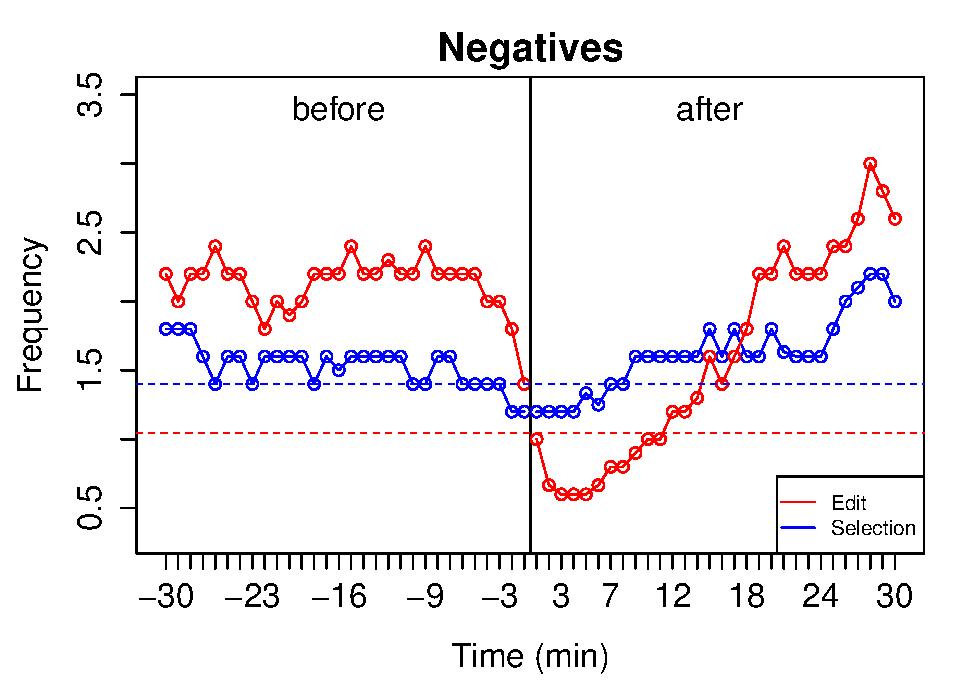
\includegraphics[valign=m,scale=0.25]{figures/udc_neg_ints} \\
%\textit{positive} (44\%): when the frequency of edit events increases after the interruption 
%	& 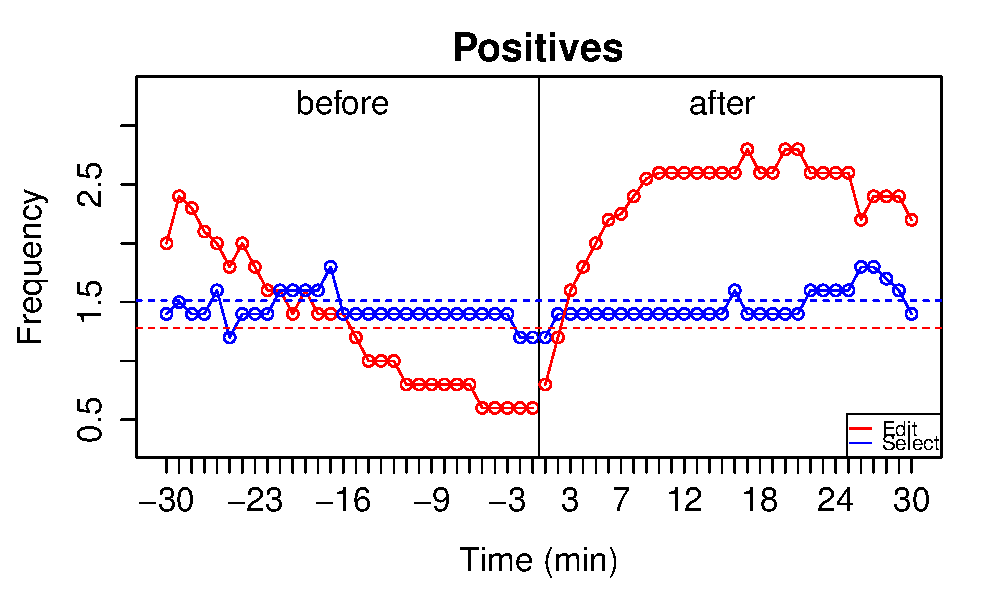
\includegraphics[valign=m,scale=0.25]{figures/udc_pos_ints} \\
%\textit{neutral} (12\%): when there is no well defined effect before or after the interruption 
%	& 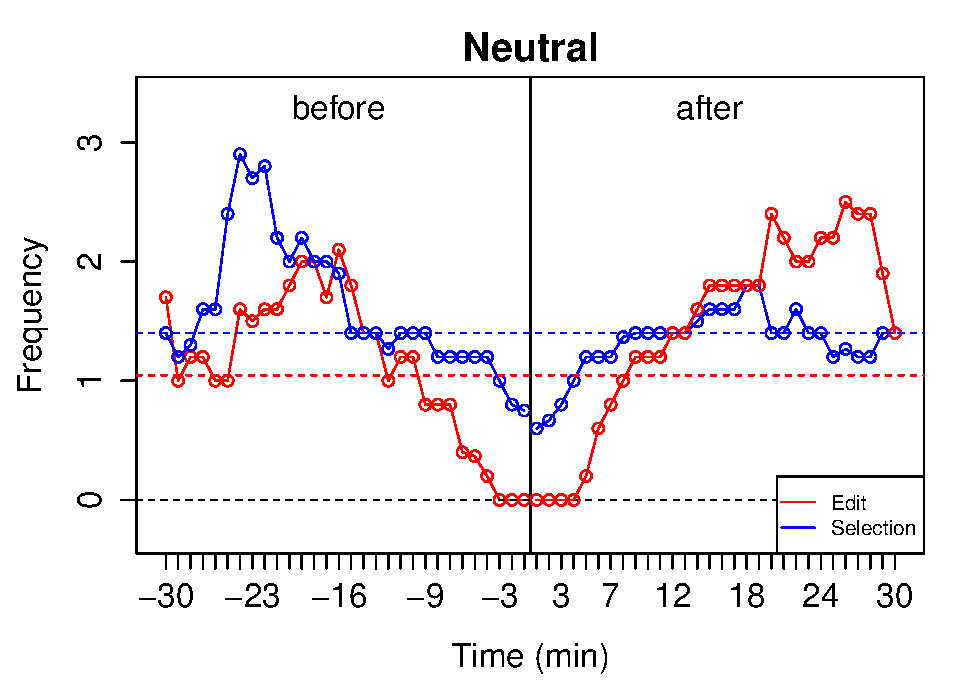
\includegraphics[valign=m,scale=0.25]{figures/udc_neu_ints} 
%\end{tabular}
%\end{table}
%
%The Table \ref{tbl:local_effect_udc} shows a similar pattern on negative, positive and neutral interruptions in comparison with the results with Mylyn. After a positive interruption both metrics tend to increase at a high rhythm until reaching the global average value. The editions per minute recover quickly, approximately 5 minutes after the interruption, but the selections per minute take a little longer to reach the global average and this metric tend to be below the average for an extended period. It is important to notice that before the interruption happens the editions per minute metric is below the average for approximately 16 minutes prior to the interruption.
%
%In contrast, when facing the effects of a negative interruption the metrics take longer to reach the median. On the contrary to facing a positive interruption, the editions per minute metric is below the selections per minute, and the former takes longer than the latter to reach the average value. Also, the editions per minute metric is above the average for the 30 minutes before the interruption. 
%
%In general, the effect of positive and negative interruptions is the inverse. The editions per minute describes better the effect and the selections do not show a major change. There is not a clear pattern during a neutral interruption.

\section{RQ4: Recovery Time after an Interruption}
\subsection{Edition and selections during recovery time}
The amount of information we have in Usage Data Collector allows us to analyze more specific sections on a programming session. We further investigated the immediate activities after an interruption that we name the \textit{recovery time}, which is a time period taken by the programmer to resume the interrupted work. We could not do this with Mylyn data, since the process involves a lot of filtering of interruptions, which left us with too few data points to analyze.

We established the recovery time as the 15 minutes period after an interruption, without considering the time consumed by the interruption itself. The length of the period was chosen according to the observations by Solingen et al. \cite{SBV98}, who explain that although it is a variable difficult to measure, estimating 15 minutes for this phase is believed to be valid. They also consider the recovery time as the third (and last) phase of an interruption; the first one is the occurrence phase, or the start interruption, followed by the handling phase that contains all the activities required by the interruption.

Furthermore, Iqbal and Horvitz \cite{IH07} conclude, after observations from field study, that the recovery time can last between 10 to 16 minutes, depending on the interruption. They speculate that this time is necessary to refocusing cognitive resources lost during the diversion.
%\RR{Add details of that paper to better justify}

In order to execute this analysis, it was necessary to make a selection of the interruptions that have a period after it of at least 15 minutes of recorded work, before another interruption occurs. After this query we obtained 5,684 valid interruptions from a total of 110,077.

From those valid interruptions, we split the time after the interruption into two phases: 

\begin{itemize}
	\item \textit{Recovery time}: the period after the interruption of 15 minutes in length.
	\item \textit{After recovery time}: the period after the recovery time until the next interruption.
\end{itemize} 

Following this procedure, the recovery time was split in three phases of five minutes each to be able to analyze the evolution through this phase on detail. Also, the period after the recovery time was split into the following phases:

\begin{itemize}
	\item \textit{Before interruption}: a period of 10 minutes before the next interruption.
	\item \textit{Peak}: the time between the recovery time and the before interruption phase.
\end{itemize}

Splitting the recovery phase into three phases allows us to analyze in detail the evolution of productivity and identify the immediate activities after the interruption, which will be helpful later. On the other hand, the before interruption phase represents the time where the productivity drops just before the next interruption, as seen in the results on RQ3. The peak phase is where the productivity should be reaching its maximum, as the programmers are not taking actions to retake the lost mental model or preparing for an interruption. The Figure \ref{fig:recovery_afterRecovery} shows how the time after the interruption was split into phases.

\begin{figure}[!ht]
	\centering
	\begin{tabular}{c}
		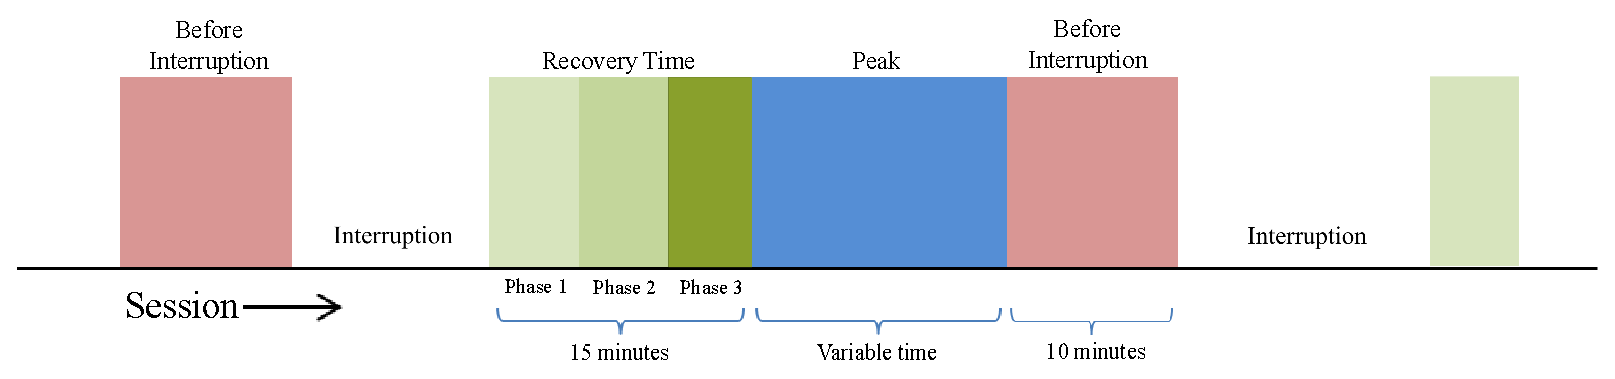
\includegraphics[width=.9\linewidth,clip=, angle=0]{figures/udc_after_Interruption} \\
	\end{tabular}
	\caption{Graphic showing how the time after an interruption was split. }
	\label{fig:recovery_afterRecovery}
\end{figure}

The duration of the peak varies among the also called working spheres \RR{add details}, as mentioned by Gonzalez and Mark \cite{MGH05}. On average, the peak lasts for 12 minutes, while the maximum registered is of 145 minutes. The distribution of duration of the peaks is reported in Table \ref{tbl:dist_peaks}.

\begin{table}[ht!]
	\small
	\renewcommand{\arraystretch}{1.3}
	\caption{Quartiles of the distribution of the duration of the peak phase.}
	\label{tbl:dist_peaks}
	\centering
	\begin{tabular}{l |c | c |c} 
		quartile & $25\%$ & $50\%$ & $75\%$ \\  
		\hline 
		 value (min) & 3.38 & 8.05  & 16.31   \\   
	\end{tabular}
\end{table}

%Considering the results obtained on the local analysis of an interruption, we can conclude that before an interruption it is common to have a reduction of both editions and selections per minute. Therefore, the \textit{After Recovery Time} time was split into two phases as well: one that takes the time where the metrics drop which happens 10 minutes before the next interruption (labeled as  \textit{Before Interruption}), and the time before that, which is the peak of the session after the Recovery Time. The duration of the phase \textit{Before Interruption} was chosen with the conclusions after the local analysis around the interruptions. 

We can see in the Figure \ref{fig:box_recovery_udc} the evolution of the metrics through
the phases. The three metrics show a tendency to increase and reach a maximum between the last phase of the recovery time and the peak of the session. Moreover, the fall of the productivity on the last minutes before the next interruptions agrees with the observations on the local analysis of the time around an interruption. From this we can conclude that the first five minutes after an interruption and the moment before the next one are the are the phases where productivity is more affected, while the phases around the peak are where the productivity is more favorable.

\begin{figure}[!ht]
\centering
\begin{tabular}{c}
\minipage{0.33\textwidth}
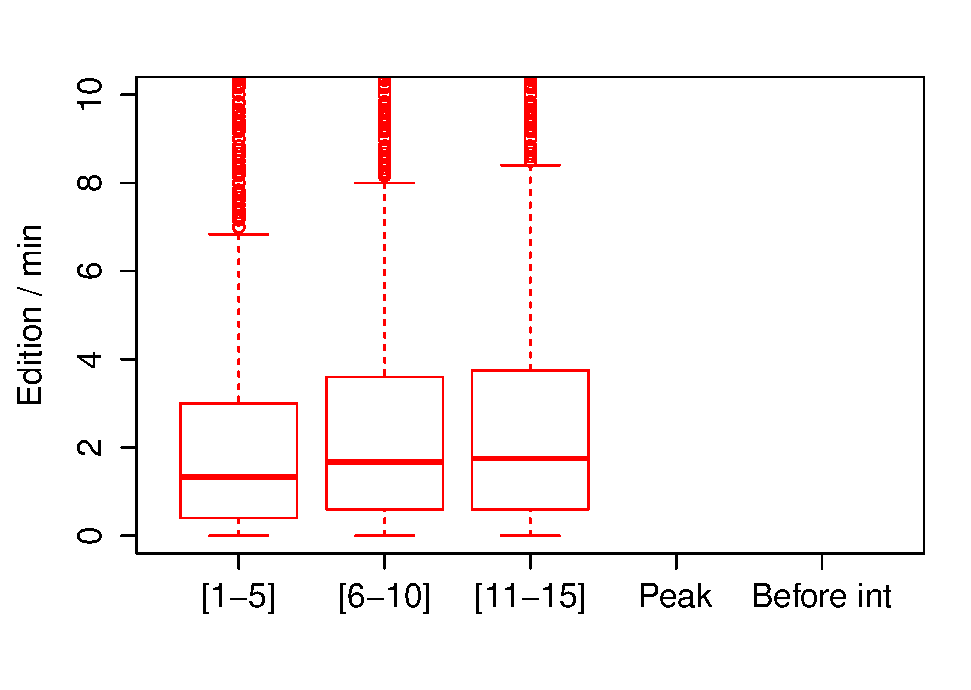
\includegraphics[width=\linewidth,clip=, angle=0]{figures/udc_box_recovery_edit}  \\
\endminipage\hfill
\minipage{0.33\textwidth}
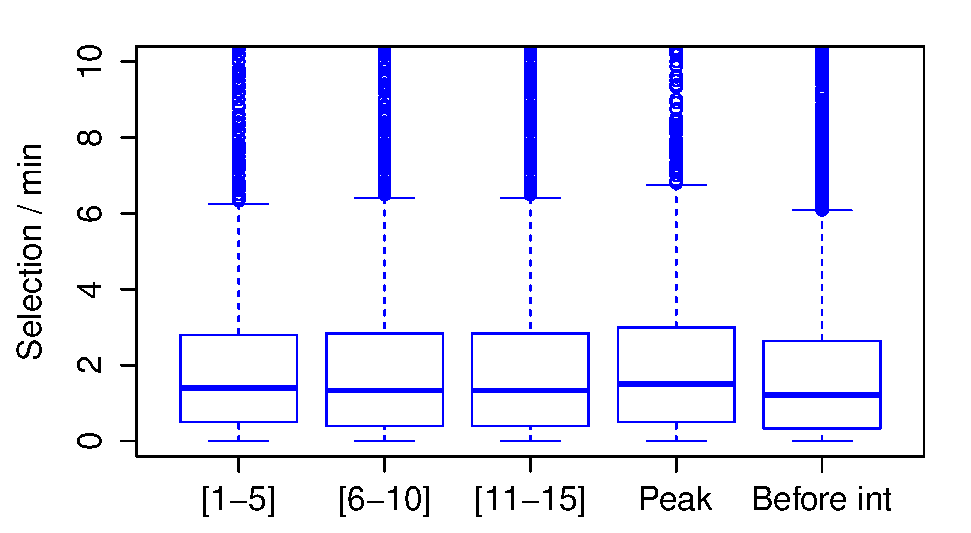
\includegraphics[width=\linewidth,clip=, angle=0]{figures/udc_box_recovery_sel}  \\
\endminipage\hfill
\minipage{0.33\textwidth}
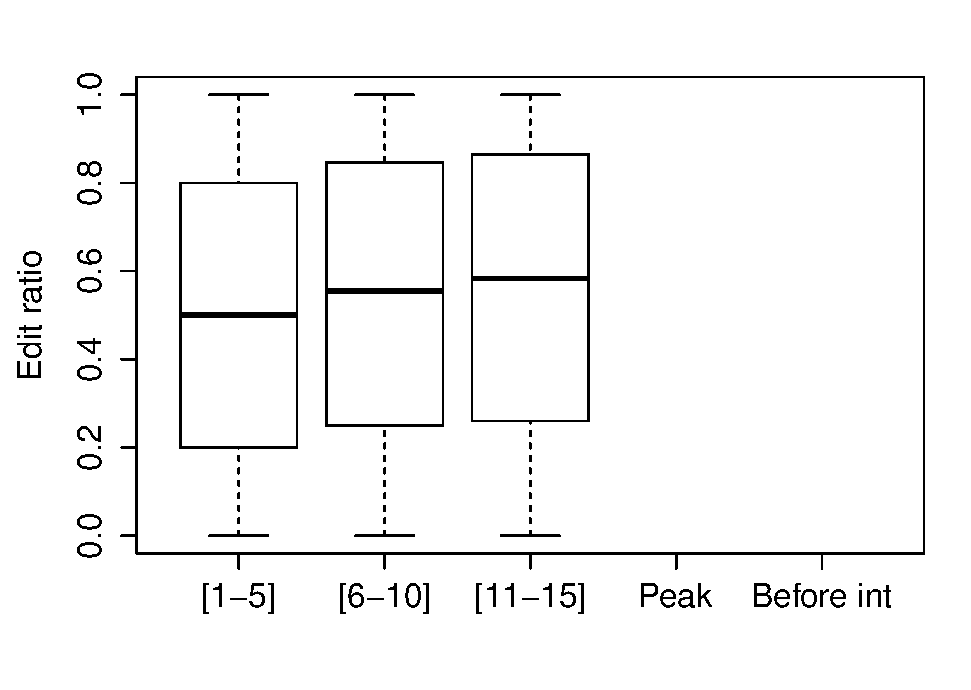
\includegraphics[width=\linewidth,clip=, angle=0]{figures/udc_box_recovery_ratio} \\
\endminipage\hfill
\end{tabular}
\caption{Boxplots showing the detailed evolution of editions, selections and edit ratio during recovery time and after recovery time. }
\label{fig:box_recovery_udc}
\end{figure}

\section{RQ5: Common events during Recovery Time}

In RQ3, we saw different patterns of activity around positive and negative interruptions. In particular, the edits per minute were higher after a positive interruption; on the contrary they were lower after a negative interruption. The effect is even more marked in the immediate minutes after the interruption, as can be seen in the Figure \ref{fig:box_recovery_effect_udc}.

\begin{figure}[!ht]
	\centering
	\begin{tabular}{c}
		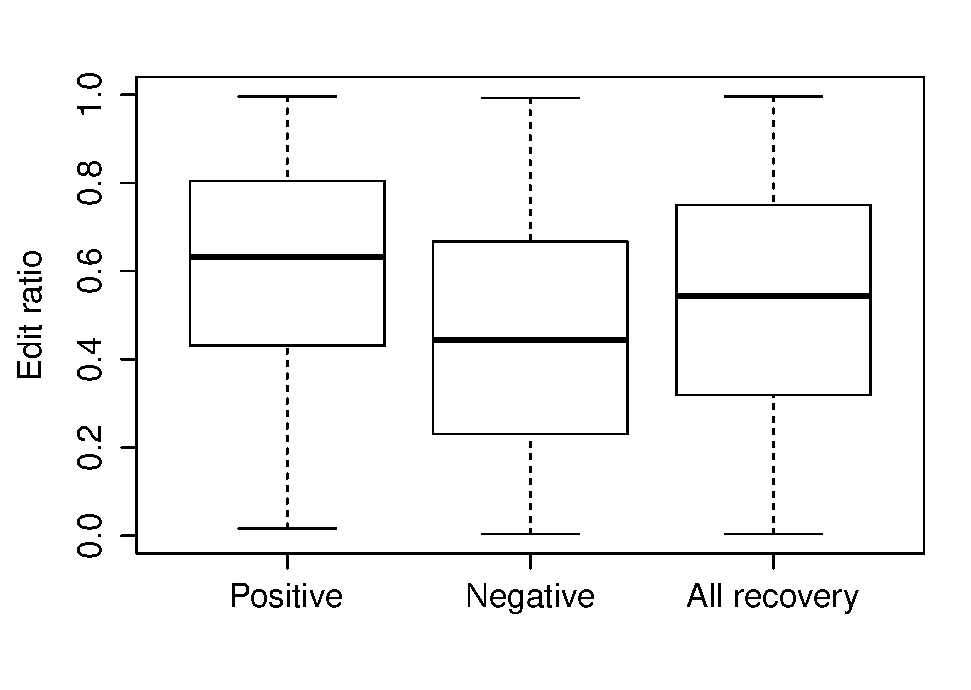
\includegraphics[width=.5\linewidth,clip=, angle=0]{figures/udc_box_recovery_pos_ratio} \\
	\end{tabular}
	\caption{Boxplot of the edit ratio during recovery time after a positive or negative interruption, compared to the edit ratio overall. }
	\label{fig:box_recovery_effect_udc}
\end{figure}


The presence of this pattern and the important difference observed in Figure \ref{fig:box_recovery_effect_udc} led us to investigate the effect more closely. To this aim, we performed an exploratory study of the activities performed by programmers during the recovery time of an interruption. This is possible due to the high variety of events present in the UDC dataset, which can tell us a lot more about the type of activities developers do. Indeed, the UDC records individual commands that the developers issued in the IDE. The commands are very descriptive in the kind of activity that they represent. 

The goal of the exploratory study then was to better understand whether the type of activities taken after an interruption were indicative of different types of activities for each type of session, and also whether these different kinds of activities supported our earlier hypotheses explaining why the two patterns of interruptions were present. Assuming that different commands represented different types of activity, the assumption was that the frequency of a given activity---as represented by the commands used to carry it---would vary between the different types of sessions.

A first challenge that we encountered was that, similarly to the earlier research questions, the high number of different commands made it hard to infer broader trends. We hence created an additional classification of the commands we encountered in the activity logs. In a similar manner to the first classification, we followed an iterative process involving two of the authors to classify the events in these categories. Differently to the first classification, we did not limit ourselves to a restricted number of categories: rather, we let the classification emerge from the iterative process. We ended up with 11 categories, as described in Table \ref{tbl:new_events_udc}.

To better understand the reasons of the difference between positive and negative interruptions, we did an analysis of the common events during recovery time, depending on the nature of the interruption. For this we created a new classification of events on a lower level that takes into consideration what kind of activity is performed by the programmer. The new classification contains the categories described in the Table \ref{tbl:new_events_udc}. This table also contains the frequency per minute of the more frequent event on that category. 

A more detailed description of each category follows.

Category \emph{high-nav} regroup events indicative of program exploration activities, such as switching between two files (usually classes), browsing a list of methods, using the outline tabs in Eclipse, etc. This category regroups most but not all usages of the views surrounding the main editor view, as well as menu items such as going to the declaration of an entity, browsing references to an entity, etc.

Category \emph{file} regroup events related to file management, such as opening and saving files, refreshing its contents and editing its properties. This kind of activity is indicative of program editing in the sense of (mostly) saving files.

Category \emph{edit-text} regroup most commands related to text edition, such as inserting or deleting characters, words, copy and paste, etc. This category is clearly indicative of program editing activities, as it regroups events that relate to the modification of low-level source code.

Category \emph{debug} is concerned with events that occur during debugging sessions, such as setting and removing breakpoints, stepping in the source code, going backwards/forwards, stepping into the execution of a method, etc. This category is clearly related to program understanding. 

Category \emph{text-nav} regroups events related to text-level navigation, such as moving to the next word, to the beginning/end of lines, or up/down a line. If this category includes navigation activity, it is still related to low-level artifacts as it represents navigation over single files, and usually small distances (characters or lines). On the contrary, category \emph{high-nav}, is related to the navigation between more abstract program elements (classes, methods, packages, interfaces), rather than low-level source code. As such, \emph{text-nav} is more closely related to code editing, while \emph{high-nav} is more closely related to program understanding.

Category \emph{search} and \emph{find-replace} are both concerned with search activities, although there are subtle differences. \emph{search} regroups most kinds of search tools, such as text search, or searching code entities (types, packages, methods). As such, it is more to be seen as a high-level program navigation tool (the search results may span several files and are presented in a view that allows quick access to the entities---using such a view is classified in the \emph{high-nav} category). On the other hand, \emph{find-replace} concerns commands that are usually employed for text navigation and more particularly to perform editions (systematically replacing occurrences of a string with another). If the first category is related to program exploration, the second is more related to program edition. There is a caveat here, as it is possible to use \emph{find-replace} commands only to find elements, which is more indicative of program exploration; however, the UDC dataset does not allow us to distinguish these usages.

Category \emph{perspective} deals with events related to perspective change in Eclipse, such as switching from the coding to the debugging perspective, or vice-versa. Eclipse allows the user to program in different environments, like enterprise, mobile and Web. It also supports activities regarding other kind of roles, like testing, design and database management. Each of this environments and roles might require to open a different perspective, so having events regarding a perspective change is an indicative of the different roles that a user has.
As such, we have no expectation as to whether this kind of activity is more indicative of program understanding or program editing. % \RR{or do we?}

Category \emph{control} contains events related to version control (commit code, update code, comparing differences, resolving conflicts). This is hence related to finishing tasks, rather than editing or understanding code. 

Category \emph{refactoring} regroups usage of refactoring tools (rename, move methods, extract methods, etc). This is indicative of edition activities in the current piece of code, but it can also affect outer elements and require to verify the changes, implying low and high level navigation. Since automatic refactorings in the IDE are behavior-preserving, the need to verify the changes is lessened. As such, we consider these events to be more indicative of program editing than program comprehension.

Category \emph{clean-build} regroup events related to build system usage (build the system, clean the build, run the build, the tests, etc). This is indicative of activities in which the programmer expects the program to be in a testable state, and not directly to program editing or understanding. This kind of events may also be automatically executed as part of a greater process. For example, when beginning a debugging session, the IDE might execute a clean and build action at first. 


With these categories described, we continue with describing the hypotheses we made earlier when we observed the positive and negative patterns, namely that:

\begin{enumerate}
\item \emph{Negative} interruptions---having higher overall activity before the interruptions rather than after it, and a lower edit ratio as well---could be indicative of actual interruptions. That is, a programmer is interrupted in his normal course of work, and needs to rebuild it's mental context after the interruption, performing additional program comprehension before resuming programming.
\item On the other hand, \emph{Positive} interruptions---with higher activity after the interruption, and a higher edit ratio---could be indicative of information-seeking behavior. Programmers, noticing that they are encountering a problem that they are not able to fix on their own, may look for outside help (asking an expert, querying a question and answer site such as Stack Overflow, etc), and once a solution is found, resume their work in the IDE in a much more productive manner.
\item \RR{What about debugging sessions?}
\end{enumerate}

We would then expect that certain types of interruptions would feature some events more frequently than other ones. For instance, after a negative interruption, we would expect more program navigation events (indicative of program comprehension), while after a positive interruption, we would expect more programming activity since the problem that the programmer encountered was solved. In short, we expect that for some categories of events, there will be differences between the types of events. We put this hypothesis to the test by calculating the frequency of categories of events after positive and negative interruptions, and also compared it with the overall frequencies of the events. We describe how we computed these frequencies in the following.
% -recall hypotheses
% - explain frequencies
% - present results
%- clear categories have clear outcome one way or the other
%- mixed categories have mixed outcomes
%=> overall pretty good then!


%\begin{table}[ht!]
%\tiny
%\renewcommand{\arraystretch}{1.3}
%\caption{New category of events. }
%\label{tbl:new_events_udc}
%\centering
%\begin{tabular}{|p{2.5cm}|p{6 cm}| p{1cm} |}
%  \hline 
%category & description & usage (\%)\\  
%  \hline 
%    \hline 
%    high-nav & High-level navigation through classes, windows and artifacts & 25.9 \\
%    edit-text & Text edition events & 19.7 \\
%    debug & Events executed during debugging sessions & 11.7 \\
%    text-nav & Low-level text navigation & 9.4 \\
%    file & Management of files (saving, closing, opening, etc.) &	8.9 \\
%    control & Source control events & 7.6 \\
%    refactoring & Refactoring events & 5.1\\
%    perspective & Change of perspectives in Eclipse & 4.1  \\
%    search & Text or code search & 2.8 \\
%    find-replace & Search and replacement of text or code entities & 2.5 \\
%    clean-build &  Events related to the build system (clean, build or run a project) & 2.3\\
%\hline
%\end{tabular}
%\end{table}

\begin{table}[ht!]
	\small
	\renewcommand{\arraystretch}{1.3}
	\caption{New category of events. }
	\label{tbl:new_events_udc}
	\centering
	\begin{tabular}{|p{2.5cm}|p{8 cm}| p{2cm} |}
		\hline 
		category & description & frequency \\  
		\hline 
		\hline 
		high-nav & High-level navigation through classes, windows and artifacts & 9.1 \\
		file & Management of files (saving, closing, opening, etc.) &	8.9 \\
		edit-text & Text edition events & 8.1 \\
		debug & Events executed during debugging sessions & 3.3 \\
		text-nav & Low-level text navigation & 3.1 \\
		search & Text or code search & 0.6 \\
		find-replace & Search and replacement of text or code entities & 0.6 \\
		perspective & Change of perspectives in Eclipse & 0.5  \\
		control & Source control events & 0.4 \\
		refactoring & Refactoring events & 0.3\\
		clean-build &  Events related to the build system (clean, build or run a project) & 0.2\\
		\hline
	\end{tabular}
\end{table}

The first thing we noticed is that while some events are used by all users, some events are used heavily by a minority of users and not by others (this matches the observation of Murphy-Hill et al., and by ourselves, that many development tools are under-used \cite{XXX, YYY}). For example, the event \textit{copyLineDown} is more frequent than the \textit{rename} event, but the former is only used by 2.4\% of the users and the latest by 25.2\% of them. As such, we calculated the frequency of event taking into account how commonly used they were.

We calculated the weighted average of every event based on the frequency of execution during the first phase of recovery time after a positive or negative interruption, and the percentage of users that make use of that event (so that events that are used by very few users do not distort the results). The weighted average was calculated as: $$\bar{x} = \frac{\sum_{i=1}^{n}w_ix_i}{\sum_{i=1}^{n}w_i} $$where $x_i$ is de frequency of execution of the event $i$ and $w_i$ is the percentage of users that uses the event. This balances the average of execution for events used by a small number of users. 

To get a baseline, the same frequency calculation was made for the entire dataset, without distinction of the location of events in the session. We then compared the weighted average changes to have evidence of what kind of events are more often executed after a positive or a negative interruption. The Table \ref{tbl:stats_events} shows the results, and is explained below.

\begin{table}[ht!]
\small
\renewcommand{\arraystretch}{1.3}
\caption{Weighted frequency of execution after positive or negative interruptions. }
\label{tbl:stats_events}
\centering
\begin{tabular}{|p{3cm}|p{2cm} |p{2cm}|p{2cm}|} 
  \hline 
category & positive & negative & all \\  
  \hline 
\multicolumn{4}{c}{\textit{Most common events after a positive interruption}} \\
    \hline 
edit-text &  \textbf{34.75} & 22.35 & 26.62 \\
file &  \textbf{10.56} & 9.53 & 10.01\\
refactoring & \textbf{1.29} & 0.84 & 1.01 \\
perspective & \textbf{0.38} & 0.30 & 0.35  \\
    \hline 
\multicolumn{4}{c}{\textit{Most common events after a negative interruption}} \\
    \hline 
high-nav & 7.84 & \textbf{10.14} & 8.74  \\
find-replace & 1.26 & \textbf{1.47} & 1.11 \\
debug & 3.08 & \textbf{7.81} & 6.35  \\
search & 0.57 & \textbf{0.96} & 0.73 \\
clean-build & 0.42 & \textbf{0.62} & 0.56  \\
    \hline 
\multicolumn{4}{c}{\textit{Less common events after a positive or negative interruption}} \\
    \hline 
text-nav & 14.20 & 12.89 & \textbf{16.13} \\
control & 1.21 & 1.75 & \textbf{1.82} \\
\hline
\end{tabular}
\end{table}

After a positive interruptions the events belonging to the \emph{edit-text} category, the \emph{file} category, the \emph{refactoring} and the \emph{perspective} category, are more frequent than in the average. In addition, these categories of events are less frequent than the average after a negative interruptions. Of these four, the two categories with the largest differences between positive and negative interruptions are \emph{edit-text} and \emph{refactoring}. Both of these categories are much more clearly associated with edition activities than program comprehesion, and thus fit the previous hypothesis. Of the two other categories, \emph{file} management is also related to program edition activities, why the role of the \emph{perspective} category is still to clarify.

After a negative interruption, the \emph{debug}, \emph{search}, \emph{high-nav}, \emph{find-replace}, and \emph{clean-build} are all more common than average. Of note, the \emph{find-replace} category is also more common in positive interruptions. The three categories of \emph{debug}, \emph{search}, and \emph{high-nav} are clearly associated with program comprehension rather than program edition. The \emph{clean-build} category is not strongly associated with program comprehension, but it is however associated with debugging activities. The \emph{find-replace} category which is more common in both positive and negative interruptions can be, as explained above, both used for find-and-replace text editions, and also for conventional search, which could explain its presence in both kinds of interruptions.

Finally, the \emph{text-nav} and \emph{control} categories are less common in both positive and negative interruptions than in the average. We were somewhat surprised that \emph{text-nav} was less common in positive interruptions than the average, as we expected it to be associated with program edition behavior. We note that it is however more frequent in positive interruptions rather than negative interuptions. Additional exploration is necessary to understand the behavior of the \emph{control} category.

Summing up, we can conclude that edition-related activities are indeed more frequent after a positive interruption, while comprehension-related activities are more frequent after a negative interruption.  These categories of events agree with our previous hypothesis that positive interruptions are related to information seeking behavior: programmers would interrupt their IDE activities when encountering a roadblock, find the information elsewhere (from the internet, an expert, etc), and return to the IDE with an increased productivity. This also agrees with the literature \cite{PR11, LVD06}. The categories common after nagative interruptions  also agree with our hypothesis that negative interruptions are related to actual task switches where context needs to be rebuilt afterwards, an activity that involves program comprehension \cite{MMLK14, PR12}. %\RR{refs here}.

After a positive interruption, we can see that the more common activities are text edition, refactoring, file management and, to a lesser extent, navigation around perspectives. On the other hand the navigation around classes, find and replace, searches, debug and clean and build are actions more common after a negative one. The navigation in the code and control version activities are more common after the recovery time, having a lower frequency during a positive o negative interruption. Of course, this exploratory study does not allow us to confirm these hypotheses. However, the evidence we have discovered so far does not disprove them, which means that our confidence in these hypotheses is higher as a consequence.

%We can conclude that after a positive interruption there are more assertive actions with a clear intention like refactoring a class or saving all changes; these activities are related to program edition. After a negative interruption, there are more uncertainty and doubt judging by the activities performed like debugging, searching for text or navigating around classes; these are activities related to program comprehension. 

%It is noticeable the relation between type of events. For example, it is natural to think that if there are many debugging events there are also a lot of clean and build events, as they are necessary to begin a debugging session and in most cases it is automatically performed by the IDE. There is also a link between high level navigation and debugging because navigating into a method may take the programmer to another class.

\section{Discussion}

\paragraph{Comparison of the datasets}
Although they represent the same kind of information both Mylyn and UDC datasets have some peculiarities that make them unique that we discuss here.

The interaction data recorded by Mylyn is the basis for a recommendation tool, and is focused on Java projects. On the other hand, the interaction data recorded by the UDC is only used for diagnostic purposes, and is much more generic. For instance, the UDC has interaction data from Java, Web, and mobile developers, and more specific roles like back-end developers, testers and C++ or PHP users. 

As the UDC was installed by default on all the Eclipse distributions from 2008 to 2010, the size of the information collected is several orders of magnitude larger than the Mylyn dataset, which was collected since then on a few dozen of developers who installed it voluntarily and contributed to the Mylyn and Eclipse projects. This makes of the UDC data a better source of information to analyze phenomenons on a wide scale.

The UDC and Mylyn also offer different levels of details: while the UDC records fine-grained type of events, Mylyn records the entity that were affected by the events (Java packages, classes, and methods). On the other hand, Mylyn has essentially two types of events of interest (edits and selections), while the UDC has no information about the entities that were affected.

%We can also have more details about every event which allows us to imply more things well beyond the role or language of preference of the programmer.

%On one side we have Mylyn a low level monitor to capture interaction data to better fix bugs for Eclipse projects. And in the other hand Usage Data Collector, a low level events monitor as well but with a more general approach. 


%Begin installed by default is also a disadvantage for UDC as many of the data is actually garbage. For example, there are a lot of users that have only a few events registered, or the work sessions tell us very little about the actual coding tendencies of the programmer. With Mylyn we can be sure that most of the data was captured under the assertiveness of having interaction data logged for further analysis.

%On this particular scenario, an advantage of Mylyn is that we had a predefined classification of the events and saved this process made with UDC. But if we expect to do a low level classification like the one on the analysis of common events during Recovery Time, then UDC is a better option. This is probably one of the causes in the difference of effects on the results (more pronounced with Mylyn) because we used a different criteria to chose between Edition and Selection when classifying the events.

\paragraph{Comparison of the results}

We conducted a replication of the results of RQ1, RQ2 and RQ3 with the additional dataset. If we noted similarities in the observations across both datasets, it is important to discuss the differences in the size of the effects that were observed: the overall effects observed were larger for the Mylyn dataset than for the UDC dataset.

The fact that all the observations go in the same direction lends us more confidence in our conclusions. However, the reduced magnitude of the effect gave us pause. We can think of several reasons for this behavior:

\begin{itemize}
\item The models are not directly comparable: Mylyn records edition and selection events directly, while the UDC records a broader array of user activity. As such, our classification of UDC events as edits, selections, or other, does not exactly replicate the way the Mylyn model operates. It is possible that some events are more frequent in the UDC than in Mylyn, for instance. We debated several ways to fine-tune our model of the UDC data, including weighting some UDC events more than others, but ultimately decided against doing so. As the models are not directly comparable, we primarily focus on intra-model comparisons.
\item The (comparatively) small size of the Mylyn dataset may have favored outliers: since there is data from dozens of developers only in the Mylyn dataset, a few outliers may have affected the results. The UDC model is however based on 1,000 UDC users.
\item Non-java users in the UDC: A small portion of UDC users were not primarily programming in Java; some were using C++, PHP, web frameworks, or a report generation plugin known as BIRT. These may have had an impact on the results.
\end{itemize}

\paragraph{The effects of multitasking}
Certainly, work fragmentation is not a synonym of lower productivity rates. Multitasking can allow the worker to use dead periods of the project where there is a decrease of the required activities and do tasks related to other projects, increasing the efficiency and productivity \cite{ABV12}. At some level, switching between tasks can provide the needed arousal and alertness to improve the productivity, but higher levels of multitasking can be detrimental and cause a negative effect. Moreover, as the number of switches between tasks increases, the effectiveness degrades in a linear fashion \cite{AB12}. 

Furthermore, the results indicate a clear diminish of productivity when facing interruptions, but with a high number of interruptions the change of productivity stops decreasing. This could be reflecting what observational studies tell us about multitasking, which is that with higher number of interruptions (increased multitasking) the productivity stops being affected and might increase. The latter actually occurs in the results but the effect is too subtle. 
We intend to reflect the effects of work fragmentation by classifying the interruptions into negative or positive, and in the results we can see a difference in productivity and the kind of activities performed.

\paragraph{Comparison with observational studies}
Our theoretical foundations are based on observational studies performed on information workers' development environments \cite{MGH05, IH07, LVD06, PD10}. These findings helped us understand the response to work fragmentation according to the recorded user activity, and it was possible to made a relation between the user's data and the phenomena that occur on the working places described in the studies.

Observing the user activity throughout a working session might be the best way to understand the effect of events that occur on the working place, like work fragmentation. However, implementing a study of this kind can be very expensive, for the time and material need. For example, to have the same amount of information we have with UDC it would require to monitor the user activity for a year or two and have a record of all the activities performed, like the number and duration of the interruptions. Moreover, this kind of research require on-site studies, exhaustive monitoring and interviews, which in some cases could be expensive or difficult to perform.

On the other hand, analyzing interaction data is a convenient way to understand almost the same kind of events on the environment. Usage data describes the history of activities of the programmer and it is possible to analyze the effect of events, as shown in this work. The problem with this is the lack of context of the events and, in our case, the lack of information of the programmers to enrich the results. Hence, we can not guarantee that an interruption was an actual interruption of work; due to the definition of an interruption, it could also be a change to a Web design tool, server configuration tool or the browser, which are common activities in Web developers and not necessarily detrimental to productivity.

The best might be to find a middle ground between observational activities and analysis of usage data. It is helpful to enhance the results using information provided directly by the participants via interviews, like the work done by Fritz et al. \cite{FMH07}.

\section{Threats to Validity}
The main threats to the validity of our study are construct validity threats due to the operational nature of the data recorded by Mylyn and the UDC \cite{M14}. Most of them are mentioned above but recalled here for convenience.

For the Mylyn dataset, the main threat to validity is due to the exclusion of development session with aggregated information. We deemed that disaggregating the data as was done in other work~\cite{YR11}  was not appropriate as we do not know the exact distribution of aggregated events in time, which is very important for this study. We thus elected to filter out part of the data. We have not found evidence of bias due to this but it may still be present.

Another threat comes from the metrics we use. Our choices are limited by the data recorded by Mylyn. We believe our three indicator (edits per minute, selections per minute, and edit ratio) provide a reasonable measure of productivity (especially with the addition of edit ratio, used in other work \cite{KM06}). However we can not exclude that other indicators of productivity (such as actual changes~\cite{RL10}) may yield different results.

As we mentioned before, the edit ratio has been used in previous work as an indicator of productivity, but it doesn't describe well the true level of productivity of the programmer. The edit ratio is the amount of coding activities that the programmer performed in comparison with the other activities, but a productive programmer may not solely code; he could have other important tasks like managing a database, Web design and testing, which are activities that are not reflected as edit events.
%\RR{add a bit stuff about edit ratio to keep one reviewer happy}

We defined several thresholds empirically: 8 hours of inactivity to split a session in sub-sessions, 30 minutes as the minimum duration for a session, 3 minutes for the minimum duration of a interruption and  $\geq$ 12 minutes for prolonged interruptions. We also tested with other close values and obtained similar results. However, a large variation of these thresholds might significantly alter the results. 

We acknowledge that our separation of sessions in short and long interruptions is not perfect, as it is based on the presence of at least one long interruption, and nothing more. Other factors present in the group of sessions with at least one long interruption may contribute to the observed effect (for instance, these sessions may also have more interruptions overall).

%It was very uncertain to get the best technique for disaggregating of events. Since, we unknown the temporal distribution of all the actions associated to an aggregate event. For this reason, we decided not to consider this type of traces in our analysis. However, this triggers another threat, we might have discarded main data that may alter the significance of our results. 

%Other threat is related to metrics for measuring the programmer productivity. We have analyzed the interruptions over the productive work time, the number of events by minute and the ratio of editions, which can be obtained from the interaction history. Other factors, as the code lines or the bug priority, they have not been considered in this work. One reason is because Mylyn have designed for increase the productivity in this aspects~\cite{KM06}.

The study has threats to its statistical conclusion. In particular, correlation does not necessarily implies causation: the drop in productivity may not be due to work fragmentation but to other factors (such as task difficulty). The fact that our results agree with the existing literature does help in this respect. We note that our local analysis uncovered two well-defined patterns around gaps of inactivity: ones that we hypothesize are actual interruptions (negative effect post-interruptions), and the ones that we hypothesize are more likely information-seeking activities (positive effect post-interruption). This result points to two different effects and is in need of further study; the additional evidence uncovered in the UDC does support this hypothesis, since different activities appear to take place in both types of interruptions. As stated in the introduction, we were careful not to conclude that every gap of activity is an actual interruption.

We used Cohen's $d$, a parametric effect size measure, as it has defined thresholds allowing easier interpretation of the results. Other effect size measures such as the common language effect size \cite{KMW92} or $A_{12}$ \cite{RRT12} may slightly alter the discussion.

This study also has threats to external validity. The gathered data corresponds to a limited group of programmers, which use both Mylyn and Eclipse regularly. The set of evolution tasks considered is a subset of the ones present on the Eclipse bug report website. It may be biased one way or another. One source of bias is the impact of Mylyn itself: Mylyn has been shown to facilitate task switching and to increase the edit ratio of its users compared to non-users. In the context of this study, we hypothesize that Mylyn could reduce the effect of work fragmentation: in other words, the observed effects may be larger for non-users. Additional studies may alleviate these threats and confirm or infirm the previous hypothesis. Our additional dataset (the UDC) comes from a much larger and more varied sample of users, and does show similar behavior, which raises confidence in our results.

%which adapted their development tasks to the platform features: Eclipse IDE $+$ Mylyn Tool. However, the bug reports did not all have associated traces and the programmers did not all submit a trace. Moreover, we used approximate measures over a sample of these data that could be analyzed. Another threat regarding data are detailed in \cite{YR11}.  The biased information that we have analyzed also is a threat to our research results. 

The same threats about the metrics, implications and statistical conclusions apply on the results observed with the UDC.  Additionally, our classification of events is a possible threat, as it was based on our own criteria of what should be an Edition and Selection event. We took this liberty due to the lack of an actual pre-classification, and on the other hand the extra information available on UDC events compared to Mylyn. We took special care when establishing the classification, using an iterative process involving two authors of this paper. We also ran tests of what kind of data was recorded for specific usage scenarios of the IDE in order to better understand the nature of the dataset when particular events were unclear.  %However, the classification still depends on the definition on what an Edition or Selection event is, for it is a factor that can alter the final results. However, we had a very clear boundary between both types and were consistent on our judgments. 

The workbench activation and deactivation events were a particular issue, for they can be executed under many circumstances. We performed live test to understand how these events work and gain confidence about their precise behavior. For instance, we found that they were reliable markers of when the user leaves and returns to Eclipse---and we used this fact to accurately detect interruptions---but we had more uncertainty on other scenarios. Therefore, we decided not count them as ``system'' events, and thus only use them to define an interruption or the end of a session.

%Another threat is the random selection of users to get their data. Although a posterior filter allows us to manage with only valid sessions, we understand that this kind of data selection might be irresponsible. For future work we'll have another approach and be more selective on the information we work.


\section{Conclusions and Future Work}
This paper presented an empirical study on the prevalence of work fragmentation in software evolution tasks, and its relationship to developer productivity. The study was based on the Mylyn dataset of software evolution tasks, where work fragmentation is indicated by gaps of activity (interruptions) in the IDE, and productivity is measured in terms of the number of edits, selections, and the edit ratio. It was then complemented with data coming from the Eclipse Usage Data Collector (UDC) dataset, which offered us to complement our previous findings by analysing a larger sample of users, with a finer-grained classification of events.

We analyzed several thousands software evolution tasks, originating from several dozens of developers. Our global analysis found an inverse relationship between number and duration of interruptions and all three of our productivity indicators. These findings agree with the literature on information workers and software developers. 

A subsequent local analysis around interruptions confirmed these results as the activity around interruptions was found to be lower than average. This analysis also found two well-defined patterns around interruptions: interruptions yielding a negative effects (consistent with a real-life interruption involving an expensive context switch), and interruptions with positive effects (consistent with information-seeking behavior). Further studies are necessary to expand on these findings.

With the Usage Data Collector dataset, we replicated our previous study to compare the results obtained with Mylyn. We found the same observations on the relationship of interruptions and productivity; even though the observed effects are less marked, we reach similar conclusions.

The UDC data also allowed us to extend our study with two additional research questions related to the recovery time after an interruption, and the two patterns of interruptions we observed. 

We first analyzed the recovery time in detail, finding a higher productivity when the interruption is positive and we identified a positive evolution of the metrics as the programmer advances through this stage, reaching a peak of productivity between the last minutes of the recovery time and 10 minutes before the next interruption happens.  

In addition, we found that after a positive interruption the most common events during the first minutes of the recovery time are those with an assertive intention such as edition, refactoring and saving files. In contrast, after a negative interruption the most common events are debugging, searching and navigation around classes, which tell us about a doubtful and uncertain behavior from the programmer. These findings support out hypotheses that positive interruptions are due to information-seeking, while negative interruptions are due to context rebuilding after an actual interruption.

\bibliographystyle{IEEEtran}
% argument is your BibTeX string definitions and bibliography database(s)
\bibliography{IEEEabrv,mybib}


% that's all folks
\end{document}


